\documentclass[chaparabic,ee,ms,12pt,oneandhalf]{metu}
\newcommand{\norm}[1]{\left\lVert#1\right\rVert}
\usepackage[]{algorithm2e}
\usepackage{csquotes}
\usepackage{appendix}
\usepackage{mathptmx}
\usepackage{caption}
\usepackage{amsmath}
\usepackage{amsfonts}
\usepackage{times}
\usepackage{xr}
\author{Kadir Çimenci}
\title{Dynamic Formation Control with Heterogenous Mobile Robots}
\turkishtitle{Heterojen Robotlarla Dinamik Formasyon Kontrolü}
\date{June 2016}
\director[prof]{xxx}
\headofdept[prof]{Gönül Turhan Sayhan}
\supervisor[prof]{Aydan Erkmen}
\cosupervisor[assistprof]{xx}
\departmentofsupervisor{Electrical and Electronics Engineering Department, METU}
\departmentofcosupervisor{Electrical and Electronics Engineering Department, METU.}
\committeememberi[prof]{İsmail Hakkı Toroslu}
\affiliationi{Computer Engineering Department, METU}
\committeememberii[prof]{Ali H. Doğru}
\affiliationii{Computer Engineering Department, METU}
\committeememberiii[assocprof]{Pınar Karagöz}
\affiliationiii{Computer Engineering Department, METU}
\committeememberiv[assistprof]{Selim Temizer}
\affiliationiv{Computer Engineering Department, METU}
\committeememberv[assistprof]{Aykut Erdem}
\affiliationv{Computer Engineering Department, Hacettepe University}
\keywords{Multi Agent Systems, Formation Control, Localization, Mesh Network}
\anahtarklm{Çok Elemanlı Sistemler, Formasyon Kontrolü, Konumlama, Örgün Ağlar}

\abstract{Formation control in robotics is a growing topic where mainly research works are geared towards heterogenous swarm colonies under decentralized control or heterogenous colonies where some centralization is considered. In swarm works where decentralization is applied, it is nevertheless assumed that the agents are capable of getting global information about the whole swarm.Moreover in the literature, formation control is generally done for known fixed shapes that can be defined mathematically. However no dynamically changing shapes are envisaged and no shape transitions are clearly handled in those works. We attempt to bring a clear impact to the literature by focusing our thesis work on tracking and realising formation shapes under dynamically changing formation shape demands. Furthermore,in our thesis work, we focus on robot colonies composed of heterogeneous robots of different dynamics and sensory capabilities under decentralized dynamically changing formation control. These robots are able furthermore, to just posess local mutual interactions only with their closeby neighboring agents. Using communications with those neighbors, all agents are being able to acquire graph theoretically, information about the whole colony. Simulations in our work will be generated using the Gazebo environment modeling a rough territory. Hardware applications of our approach will also be developed.}

\oz{Formasyon kontrolü robotik alanında heterojen robot kolonilerinin merkezi yönetici birimler olmadan ya da yerel merkezi birimleri barındıran topolojilerle kontrolü konularına yönelik büyüyen bir araştırma alanıdır. Merkezi yönetim birimlerinin olmadığı robot sürüsü çalışmalarında ne yazık ki her üyenin, koloniye mensup diğer üyelerin tüm verilerine erişebildiği varsayımı yapılmaktadır.Öte yandan, literatürde formasyon kontrolü genellikle matematiksel olarak ifade edilebilen basit geometrik şekillerle yapılmaktadır. Bununla birlikte bu çalışmalarda, dinamik olarak değişen şekiller ve bu şekiller arasında formasyon geçişleri konusu yeterli olarak ele alınmamaktadır. Bu çalışma kapsamında dinamik olarak değişen şekiller için formasyon kontrolü sağlayarak literatüre katkıda bulunmayı hedefliyoruz. Öte yandan bu tez çalışmamızda, farklı dinamiklere ve sensör yetkinliklerine sahip heterojen robot kolonileri kullanarak dinamik formasyon kontrolü problemini merkezi karar verici birimlerin olmadığı bir topolojide ele alacağız. Çalışma kapsamında ele alınan kolonilerdeki tüm robotlar yalnızca kendilerine en yakın komşu üyelerle yerel etkileşimlerde bulunabileceklerdir. Komşularıyla etkileşimde bulunan üyeler, konsensus koordinat sistemi ve koloninin geri kalanı hakkında bilgi sahibi olabileceklerdir. Çalışmamız kapsamında simülasyonlar Gazebo ortamında üç boyutlu düzgün olmayan araziler modellenerek yapılacaktır. Ayrıca donanımsal gerçeklemeler içeren çalışmalar da yapılacaktır.} 

\dedication{\textit{To my family and people who are reading this page}}
 
\acknowledgments{
TODO
}


\usepackage[pdftex]{hyperref}
\usepackage[all]{hypcap}
\usepackage{todonotes}
\usepackage{graphicx}
\graphicspath{ {./images/} }
\usepackage{rotating}
\usepackage{xy} 
\usepackage{booktabs}
\usepackage{pifont}
\usepackage{color}
\usepackage{listings}
\usepackage{pdfpages}
\usepackage{array}
\newcolumntype{M}{>{\centering\arraybackslash}m{\dimexpr.25\linewidth-2\tabcolsep}}
\renewcommand\lstlistingname{XChor Language - }
\def\lstlistingautorefname{XChorCode.}
\lstset{
language = java,
basicstyle=\small,
numbers=left,
numbersep=10pt,
numberstyle=\tiny\color{black},
stepnumber=1,
tabsize=2,
showspaces=false, 
frame=single,
breaklines=true,
escapeinside=~~
}
\usepackage{float}
\restylefloat{figure}
\newcommand{\tab}{\hspace*{2em}}
\DeclareGraphicsExtensions{.pdf,.png,.jpg}

\begin{document}

% Preliminaries
\begin{preliminaries}
% If you are willing to use any custom stuff before Chapters, put it here
% Such as List of Abbreviations
% Check the abbreviations.tex for a template list of abbreviations

\begin{theglossary}{LONGESTABBRV}
\item[ABBRV] Abbreviation
\end{theglossary}

% End of Preliminaries
\end{preliminaries}
%   
% Latex content Goes Here 
% 
%

% CHAPTER 1

\chapter{INTRODUCTION}
\label{chp:introduction}

This thesis work focuses on dynamic adaptation to achieve changes in formation of swarms consisting of heterogeneous mobile robots. The term of swarm has a meaning \cite{4}, a large group of locally interacting individuals with common goals. 

Self organizing swarm researches and its applications are generally inspired from the biological systems existing in the nature. Behaviours of complex biological systems remained unresolved for a long time, until recent researches that showed individuals with supple functionalities can achieve complex tasks by cooperation \cite{2}. Biological systems (such as colonies of ants) have simple behaviours but they can accomplish very complicated collective tasks in nature quite impossible to be achieved solely by individual capabilities. Beni \cite{1} describes this collaboration of members as follows:

Collaborative robot network is not just an agglomeration of robots, they have essential characteristics, which are found in swarms of insects, that is, decentralised control, which does not require synchronisation, and individuals which are simple and (quasi) identical.

Properties of swarm robotics systems that make them unique are the simplicity of individuals, restricted sensing and communication capabilities, collaborative achievement of complex tasks, robustness and decentralization of control capabilities \cite{6}.

Swarm robotics has been studied to produce different collective behaviours to solve different tasks such as as aggregation , pattern formation , self-assembly and morphogenesis , object clustering, assembling and construction , collective search$\&$rescue and exploration , coordinated motion , collective transportation , self-deployment , foraging and others\cite{5}. Dorigo and Trianni \cite{7} are studied on controllers for aggregation of coordinated motion of the identical mobile robots called swarm-bots. Their implementation has a centralized structure in which a decision maker assigns roles to individual agents. In our work, each agent is responsible to reach global consensus on the final positions in formation which increase the robustness of the system against to individual erroneous decisions. Hou et al. is focused on controlling of a swarm within a dynamically changing formation \cite{8}. In their work, it is needed to describe a global objective function which requires analytical expression of the desired formation shape. But it may not be possible to define the desired formation shape with analytical expressions in real world applications. In this thesis work, the solution does not require the analytical expressions of the desired formation shape.  Ganesh and Lisa introduced two new strategies for collective search and exploration of fields with swarm intelligence \cite{9}. Their implementation requires a central controller to manage the individuals and this type of solution has a single point of failure system characteristic because of the dependence on single decision maker agent.   Chaimowicz and Campos proposed a new methodology which is based on a dynamic role assignment mechanism in which the robots cooperate with each other and they demonstrate this method in a cooperative transportation task \cite{10}. Their work implements a leader follower structure in which following agents has no impact on the global consensus of the swarm. This approach depends on the decisions of an individual agent and an erroneous decisions of this individual may cause the failure of whole swarm. 

There are lots of studies related with different problems in swarm robotics literature as discussed briefly. In this thesis project, we are focused on dynamic pattern formation control of swarms consist of heterogeneous robots. All agents contribute on the decision process and they collaborate to minimize the total displacement while achieving the desired formation shape. 

\section{Problem Definition}
In this thesis work, we aimed to design a formation control system with heterogeneous robots and dynamically changing complex shapes. Desired formation shapes for real time applications, such as covering an area or a search$\&$rescue operation, may not be simple geometrical shapes with analytical expressions. The solution which does not require a mathematical definition of the desired formation shape is more suitable for these type of applications. On the other hand, this formation shape may be dynamically changing to meet the requirements of the task in real time. 

In literature, formation control systems generally include a decision making process which is executed by an individual agent or a central server. This kind of approach creates a single point of failure system and this ruler may cause a failure for the whole swarm by making a mistake. In this work, it is aimed to implement a solution in which each member of the swarm contributes on the decisions and global consensus of the swarm.

Formation control systems which are implemented with swarms composed of homogeneous agents cannot achieve special tasks which requires different functionalities of individual agents. In this work, we have focused on implementing a solution with a swarm consisting of heterogeneous agents with different capabilities. 

In this work, the main idea is to propose a complete design solution to a dynamically changing formation system, including a local positioning and formation control system. Formation control system heavily depends on the position data of individual agents in the workspace. Since it is expected to have high number of agents in the environment due to the nature of a swarm, the agents are assumed to have simple structures with low capabilities including lack of certain types of sensors. On the other hand, for indoor applications it will not be possible to use satellite dependent positioning systems on agents \cite{19}. Even if a positioning solution provided for an indoor application by different methods including visual feedback(by image processing), RSS(received signal strength) etc. , it is not possible to implement this solution for each single agent in the environment due to the increasing complexity and the costs by the number of agents. In literature, formation control systems are generally designed with the assumption of the positions of each agent is known exactly. To propose a complete solution for the formation control problem, it is required to implement a localization solution for the agents to provide the corrected positions in the workspace which will be used by the formation control system. This localization process must implement a solution to correct the position data of the agents within an maximum error bound. This error bound is determined by the requirements of the formation control problem. 

\section{Motivation}
The formation control problem is defined as the collaboration of a group of agents towards maintaining a formation with a certain shape \cite{12}. It focuses on leading the individual agents of a swarm to perform  collective tasks including shape generation and formation reconfiguration while traversing a trajectory avoiding collisions. These kind of tasks are achieved with a large group of simple robots  that can cooperate with each other. Formation control of multi agent systems  is an actively growing research field.

Swarms which are used in formation control systems, can be composed of homogeneous or heterogeneous agents according to the requirements of the problem. The usage of the homogeneous agents increases the total impact and the coverage of the system in the environment. This kind of a swarm has an increased redundancy and is capable of resuming the current task in case of failures of some of the agents during mission. On the other hand, a swarm composed of heterogeneous agents has different capabilities of the agents. This kind of a system can be used in tasks which requires different functionalities has to be performed individually or simultaneously.

In real world applications there may be need for different  functionalities to achieve some specific tasks. If this is the case, one solution may be to design a sophisticated robot which includes all required capabilities for this task. In this scenario, this robot will be the single point of failure in the system and if robustness is a  vital feature for this solution, some redundant robots have to be added to the system. It is clear that the design of such an advanced robot and hold its redundant backups in the system will increase the cost of the solution. In swarm robotics concept, one of the approaches related with the usage of the heterogeneous agents is to gather some different types of simple mobile robots which have their own specific functionalities to achieve a collective task rather than designing an advanced robot for the solution \cite{99}. With this approach, the robustness of the system is increased, costs are reduced down and the reusability of the individual members of the swarm for other tasks is provided.  A project named Swarmanoid which is funded by European Commission, has an objective to implement and control of a novel distributed robotic system. The system is designed with heterogeneous, dynamically connected, small autonomous robots called foot-bots , hand-bots and eye-bots where foot-bots are responsible to transport the required materials(including other types of robots) to a specific task area and hand-bots are responsible for operations to be handled with their manipulators and eye-bots are responsible of observations and reconnaissance on the workspace. This project implements a system which has a leader follower structure in which a decision maker agent assign different tasks and roles to the other members of the swarm. Wrong decisions or the failure of this decision maker may prevent the whole swarm to achieve the desired task. In this thesis work, we have focused on a system in which each agent is responsible to contribute on the decision process.

\begin{figure}[H]
\caption{A Robot Team Consists of Eyebot, Handbot and Footbot Agents \cite{99}}
\centering
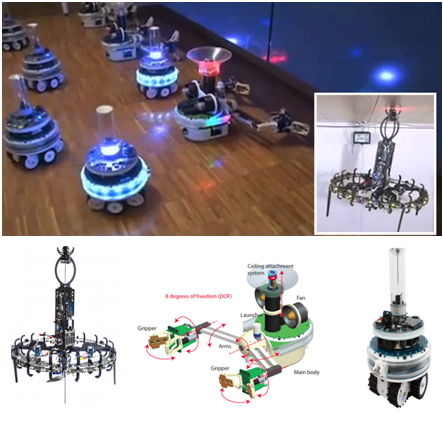
\includegraphics[scale = 1]{eyebot}
\end{figure} 
\newpage
A swarm which is composed with same type of homogeneous agents can be used to increase the total impact and the energy of an individual agent. This kind of a system can be used in missions like coverage, search and  reconnaissance etc.  Martin and Kilberg have worked on formation control and formation tracking of  microsatellites to achieve continuous coverage and improved capability. They also mentioned that small formations will reduce the fuel consumption for propulsion and expand the sensing capabilities of microsatellites \cite{15}.

\begin{figure}[H]
\caption{Sparse Aperture Formation of Micro Satellites \cite{15}}
\centering
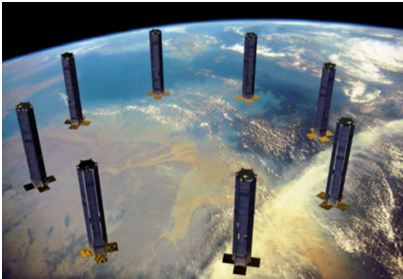
\includegraphics[scale = 1]{Satellite}
\end{figure} 

Formation control solutions has lots of usage areas such as coverage missions, security patrols and search$\&$rescue in hazardous environments etc.\cite{13}. For missions related with area coverage and reconnaissance, a group of autonomous vehicles may be required to keep in a specified formation \cite{13}.  

There are some hardware implementations to test the related formation control algorithms in real time applications. Since the formation control problem requires lots of agents in a swarm, these works have a common point of providing agents with minimal costs and sensor capabilities. The Kilobot Project from Harvard university have released their agents with the name of Kilobots and they have teams which are working on different formation control problems with Kilobots \cite{98}.

\begin{figure}[H]
\caption{Formation Control with Kilobots \cite{98}}
\centering
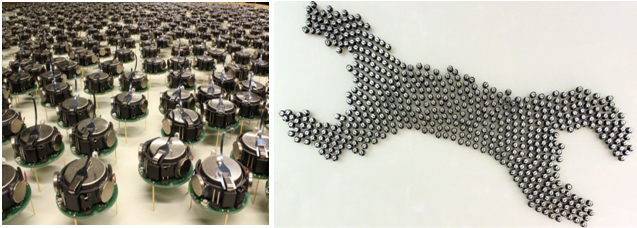
\includegraphics[scale = 0.70]{kilobot}
\end{figure}

These micro robots have a great reusability for different types of formation control problems  and they have biological inspiration from the nature in the sense of individual simplicity and power of collective behaviours. Common feature of these projects, they implement formation control systems with swarms composed of homogeneous agents. In real world applications, complex tasks may require different functionalities which can be provided by different types of robots. In our work, we have focused on implementing a formation control system with heterogeneous agents.

\begin{figure}[H]
\captionsetup{format=hang,justification=centerfirst}
\caption{
A) Swarm Robot Project from Universities of Stuttgart \cite{97}  \\
B) Colias Project from Lincoln University and Tsinghua University\cite{96}\\
C) Marx bot developed at EPFL\cite{95} \\
D)Swarm bots project conducted by  European Commission \cite{94}}

\centering
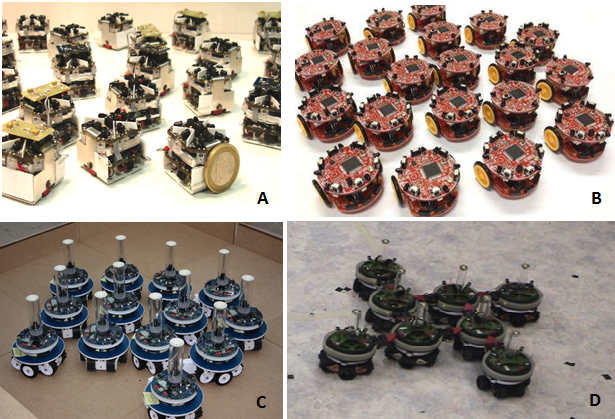
\includegraphics[scale = 0.7]{mobilerobots}
\end{figure}

    
    
  
    
Hou et al. has implemented a formation control system with dynamically changing formation shapes \cite{8}. Their approach defines a global objective function which requires the mathematical definition of the desired formation shape. But in real world applications it may not be possible to derive the analytical expressions for the desired shapes. In our work, control laws for individuals in the swarm does not require such a global objective function definition.

\begin{figure}[H]
\caption{Dynamical Formations with Global Objective Functions \cite{8}}
\centering
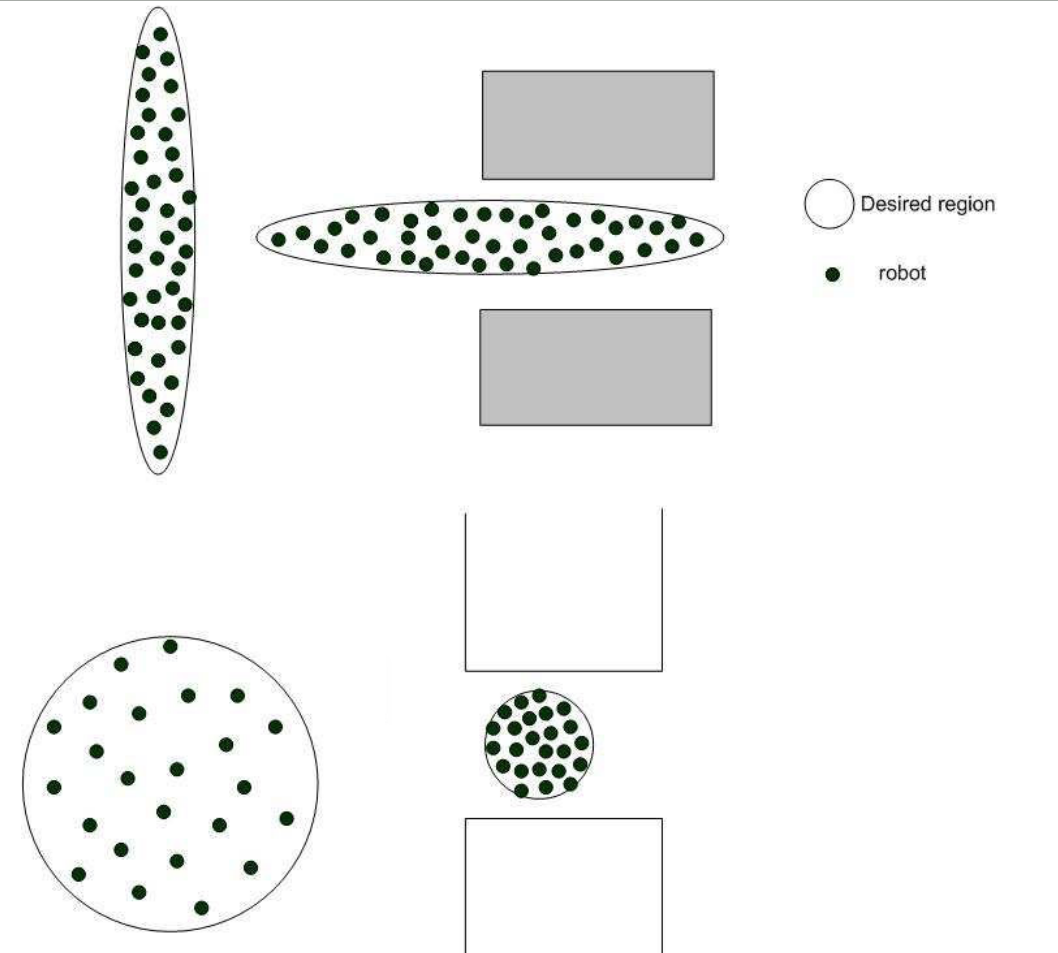
\includegraphics[scale = 0.32]{houslotine}
\end{figure}


\section{Objectives $\&$ Goals} \label{Objectives}
In this thesis work, our aim is to provide different approaches $\&$ solutions to the requirements in formation control problem.  There are mainly different types of  infrastructures which propose solutions to the formation control problems like the heterogeneity vs. homogeneity of the agents, communication structures, centralized vs. decentralized structures, swarm control strategies like behaviour based and leader-following approaches or virtual structure based approaches. 

Our main approach is to design a complete solution to the formation control problem by taking into account the requirements related with real world applications. In literature, formation control systems generally implements solutions with simple geometrical shapes \cite{8}. One of the objectives of this thesis work is to implement a solution which does not require the mathematical definition of the desired formation shape. Also it is aimed to design an algorithm which can adapt itself to the dynamically changing formations.

On the other hand, most of the related work assumes that it is possible to measure the exact positions of the agents in the workspace \cite{98,97}. Another objective of this thesis work is to implement a localization solution for the agents by assuming they may not able to measure their positions. With this approach, it is possible to provide a complete solution to the formation control problem.

Specific tasks including different missions, requires agents with different capabilities and this kind of tasks may not be achieved with swarms composed of homogeneous agents \cite{99}. In our work, one of the objectives is to implement a formation control system with heterogeneous agents. Furthermore, proposed solutions for formation control problem generally includes a decision making process which is executed by an individual agent or a central server. This kind of approach creates a single point of failure system and if this decision maker unit fails during mission, swarm cannot achieve the desired task. In this thesis work, it is aimed to implement a solution in which every agent is responsible of contributing on decisions and reaching a global consensus. 

In addition to choice of the formation control infrastructures, capabilities of the individual agents provide additional requirements and constraints while designing a formation control system. One of the most important characteristic of an agent in the swarm is its simplicity and limited sensor $\&$ communication capability \cite{6}. This approach results from the idea of achieving collective tasks with lots of simple individuals  and it is based on biological inspirations in nature like colonies of ants etc. In our work, it is aimed to propose a solution by taking into account that agents in the swarm has simple structures and limited sensor capabilities.

To achieve these objectives and meet these requirements, the goals for this thesis work are defined in the following subsections of \ref{Objectives}.

\subsection{Heterogenous Robots with Different Dynamics}
It is aimed to create a formation control system with heterogeneous agents to achieve complex tasks which require different functionalities. To accomplish this objective, it is assumed that agents have different dynamics from each other like different friction surfaces, geometrical structures, dynamics and functionalities. They have different volumes and masses and they may collide with the other ones and the obstacles in the environment.


\subsection{Communication Infrastructure}
One of the objectives in this work is to implement a localization solution for the agents. Also it is required to implement a communication backbone to execute a decentralized decision making process in which each agent reaches a global consensus. To meet these requirements, it is needed to implement a communication infrastructure in the proposed solution. By taking into account that the agents in the swarm have limited communication capabilities and can only negotiate with its local neighbors in a narrow line of sight range due to power consumption issues and their weak radio links, this infrastructure must have following specifications.

\begin{figure}[H]
\caption{Radio Links on Agents Have a Narrow LOS Range}
\centering
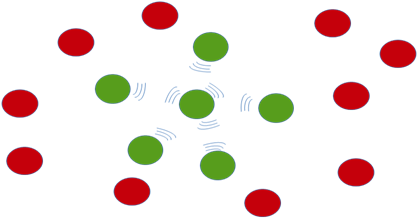
\includegraphics[scale = 1]{narrow_los}
\end{figure}

a)Communication Topology \newline
Communication topology is a wireless mesh network in which each agent relays data for the rest of the network. The network is fully connected and has routing technique where the data is propagated along a route by transporting over the nodes(member agents of the swarm).

\begin{figure}[H]
\caption{Mesh Network Between Agents}
\centering
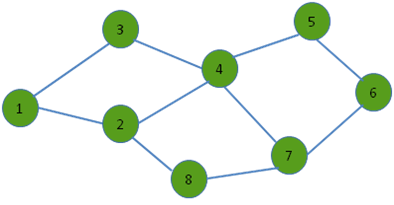
\includegraphics[scale = 1]{mesh}
\end{figure} 

b)Communication Bandwidth \newline
Bandwidth of the communication between agents is limited and nodes can only transport most critical data like heartbeats, agent IDs, type and position etc.

\subsection{ Decentralized Decision Making Process} \label{decent_decent}
Centralized formation controller systems implement a single controller  server/root node to process all the data needed to achieve the desired objectives. This type of systems achieve superior performance and optimal decisions  but they require high computational power, high communication bandwidths and are not robust due to dependence on a single controller \cite{12}. Decentralized formation controller structures have agents which are completely autonomous and responsible their own individual decisions. In this work, a hybrid centralized/decentralized controller architecture in which there is a central manager which partitions the desired formation shapes into goal states. Agents report their costs to reach these goal states and try to reach a consensus about final goal states to minimize the total displacement of the swarm.

\begin{figure}[H]
\caption{Agents Reach a Global Consensus on Goal States}
\centering
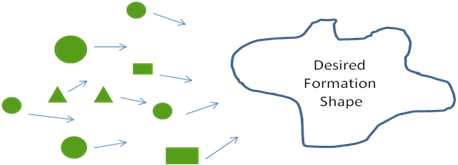
\includegraphics[scale = 0.8]{decentralized}
\end{figure} 

\subsection{Complex and Dynamically Changing Formation Shapes}
In literature, formation control systems are generally designed with a single or combination of simple geometrical shapes and they require analytical expressions of these shapes while implementing the proposed control laws for individual agents \cite{93}. Specific tasks which requires more complex shapes cannot be achieved with this approach. In our work, we have focused on designing a formation control algorithm which does not require the mathematical definition of the desired formation shape. The goal to accomplish this objective is to design a solution which does not depend on the analytical expression of the formation shape. Furthermore, in literature the general approach is to implement a solution to cover a static formation shape. In real world applications it may be needed to update the desired shape dynamically according to the requirements of the task. In our work, one of the goals is to propose an algorithm which can adapt itself to dynamically changing formation shapes.

\begin{figure}[H]
\caption{Complex and Dynamically Changing Formation Shapes}
\centering
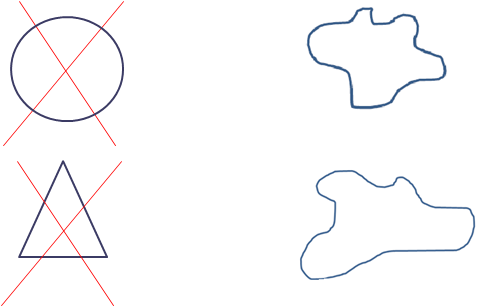
\includegraphics[scale = 0.7]{complex}
\end{figure}

\subsection{Simple Agents with Low Sensor Capabilities and Low Computing Powers}
In this project, we have assumed that the agents have low sensor capabilities and weak computing power \cite{6}. These constraints must be taken into account during the control system design, since individuals do not have a high resolution and sensitive data about the workspace and their states, and they cannot execute high level complex control algorithms.

\section{Requirements}
The goals of this project define some requirements about the implementation of the formation control system. These requirements are listed as follows:

1. Agents have to propagate their positions and velocity states with the help of inertial measurements.This process is handled with a Kalman estimator which takes the translational acceleration data as an input to the observer model .The translational acceleration data is calculated with the help of inertial measurements. 

2. Agents have to update$\&$adjust their position data with the help of agents which have positioning sensors(we call these agents position beacons) by local trilaterations.This position data is used in the estimator system as an external measurement to correct the drifts caused by propagation error of translational accelerations.

3. Agents have to update their route tables to create a communication backbone with the mesh network topology. Since agents are assumed to have low range$\&$bandwidth radio links, the propagation of a data between each agent in the swarm will be handled over this mesh network. 

4. Desired formation shape will be partitioned into potential goal states for different types of agents in shape partitioning based approaches. Performance analysis on proposed shape partitioning methods have to be done with some different criterias. 

5. Assignment of the agents to their target goal states should be done to minimize the total displacement of the agents while travelling towards the desired formation shape in shape partitioning based approaches. 

6. Simulations should be performed to compare the efficiency of different methods proposed in this thesis work. Different types of agents have to be represented with different dynamical and physical models during simulations.

7. Hardware demonstrations should be performed to illustrate the applicability of the proposed solution in real time systems. These applications may not contain the full implementation of the proposed system, but they must demonstrate a proof of concept(POC) environment.

\section{Methodology}
During the first part of the project, a local positioning system(LPS) is designed. In this system, agents which does not have position sensors, propagate their position and velocity states with their inertial measurements. Due to  drift problems on this solution \cite{91}, a position update process is handled with the help of local trilateration process. During the update phase of the solution, route tables for individual agents are determined with the help of Destination-Sequenced Distance Vector Routing Protocol (DSDV) algorithms. This process provides the required information to the agents about the position beacons which are their direct neighbors in the swarm. Position measurements are handled for each agent by local trilateration process with the help of position beacons which are direct neighbors of them. A Kalman observer is designed to fuse these propagation and update phases of the solution.

On the second part of the thesis work, formation control system is designed with two novel methods based on Bubble Packing method and Randomized Fractals method. Desired complex formation shapes are partitioned into goal states according to the heterogeneous agents in the swarm for both of these two methods. Decision process of the agents about their target goal states to minimize the total displacement of the swarm is implemented with the help of Visibility Graphs and Hungarian algorithms. Internal velocity controllers for individual agents to reach the goal states are implemented with a full state feedback method by regulating the augmented dynamical system with the gains optimized by Linear Quadratic Regulators (LQR).

\section{Contribution of Thesis}
The main contributions of thesis are:

1. Designing a local positioning system(LPS) based on local trilaterations to provide position data to the agents which do not have specific position sensors on their boards.

2. Implementing a wireless mesh network between agents in the swarm and designing a communication infrastructure and related routing algorithms to exchange the local data globally in the network

3. Implementing a formation control system with complex and dynamically changing formation shapes by using swarms composed of heterogeneous agents.

4. Designing and implementing the rules$\&$algorithms for the decentralized decision making process of the individual agents about the goal states in desired formation shape.


\section{Outline of the Thesis}
This thesis work is organized into 6 main sections. Chapter 1 introduces the main theme and the potential usage areas of formation control, while specifying our motivation and the requirements$\&$problems to meet$\&$solve related with the topic.

Chapter 2 gives literature reviews about the related works and discuss about the advantages$\&$disadvantages of the proposed method.

Chapter 3 introduces the methods and solutions used in two different parts of the problem; local positioning system and formation control system. In this chapter, routing algorithms and mathematical aspects of the trilateration process is introduced. On the other hand methods$\&$algorithms used for formation control is discussed in details.

Chapter 4 provides simulation analysis on the local positioning system and gives mutual evaluations of the performances of different methods used in formation control system.

Chapter 5 provides and discuss the details of hardware implementations and the experimental results.

Chapter 6 concludes the thesis and defines the future works related with the thesis.

% CHAPTER 2

\chapter{LITERATURE SURVEY}
\label{chp:Literature Survey}

\externaldocument{chapter1}
\externaldocument{chapter6}
\externaldocument{chapter3}
\externaldocument{chapter4}
\externaldocument{chapter5}

Formation control requires local positioning, detection of the general shape, task allocation to individual agents and task dispatching. The literature has related works in these different fields but lacks the dynamically formation control to dynamically changing shapes. This chapter is intended to motivate the need for the topic of this thesis by underlying the gap it filled by reviewing existing works in related fields. 
\section{Local Positioning Systems} \label{LPS_systems_ref}

Positioning systems are used to provide the required position data$\&$feedback to the systems where it is desired to control the location of the mobile agent in the workspace. 
These systems fall in to two main branches, global positioning systems and local positioning systems. Global positioning systems(GPS) has become increasingly popular for a couple of last decades for tracking location. In outdoor formation control applications this solution is used for positioning \cite{29}. It is a precise system depends on satellite based positioning mainly developed for direction finding and navigation.  Some of the problems encountered with the usage of GPS systems: (1) the signal from the satellites cannot penetrate to the indoor space so it doesn't perform in such areas, (2) it looses its precision in rich scattering environments such as urban areas \cite{19}.  A local positioning system can provide a position information where GPS systems are unavaliable,with the usage of signaling beacons which are placed at the exactly known locations. In indoor formation control applications this kind of approach is used for positioning \cite{96}. 




\begin{figure}[H]
	\caption{Accuracy Statistics of Different Positioning Sources \cite{20}} \label{overview_position}
	\centering
	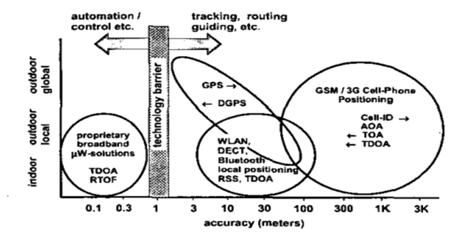
\includegraphics[scale = 0.4]{gps}
\end{figure} 

Figure \ref{overview_position} represents an overview of current positioning systems \cite{20}. Global positioning systems are widely used nowadays and they provide accuracies in the range of 3-30 meters. They further can operate in outdoor environments requiring radio signals from satellites. Differential GPS systems decrease these accuracy range below 3 meters with the help of additional local static beacons. GSM based solutions have the worst accuracy performance because they localize the nodes in the network by checking the relative signal strengths from different beacons, but they can perform in indoor environments partially \cite{20}.  Local positioning systems have the capability of working indoor environments because they use the signaling beacons which are placed at the exactly known locations \cite{20}. 

Local positioning systems has different system topologies illustrated in the Table \ref{different_top}20].

\begin {table}[H]
\begin{center}
\newcommand{\wrap}[1]{\parbox{.40\linewidth}{\vspace{1.5mm}#1\vspace{1mm}}}
\caption {Local Posititioning Systems with Different System Topologies \cite{20}} \label{different_top} 
\begin{tabular}{ |c|c| } 
\hline
\wrap{Concept} &\wrap{Concept	Definition} \\
\hline
\wrap{Remote Positioning} &\wrap{Measurement from remote site to mobile device}\\
\hline
\wrap{Self Positioning}&\wrap{Measurement from mobile unit to usually fixed transponders(landmarks)} \\
\hline
\wrap{Indirect remote positioning}&\wrap{Self positioning system with data transfer of measuring result to remote site } \\
\hline
\wrap{Indirect self positioning}&\wrap{Remote positioning system with data transfer of measuring result to mobile unit} \\			
 \hline
\end{tabular}
\end{center}
\end{table}

Two main topologies are self positioning and remote positioning systems \cite{20}.  In self positioning system a mobile device finds its own position with the help of a predetermined reference such as a starting point or a beacon node with exactly known positions. On the other hand, in remote positioning systems a mobile node locates other objects positions relative to its own position \cite{19}.   These two type of topologies can be converted to each other with the help of a communications structures integrated on the devices to share the result of position measurement and thus indirect remote positioning and indirect self positioning system topologies can be implemented. Self positioning systems can be implemented to provide position data to the individual agents in formation control problems. The approach is to distribute the position data to the individual agents from a beacon node with exactly known positions. The individual agents which do not have a positioning sensor on their boards, measure their distance to these beacons and correct their position data with these external measurements. Beacons are assumed to have a GPS sensor on their boards for outdoor applications. They are assumed to have a special tag to locate them in an indoor environment with the help of external devices such as E/O camera.




\subsection{Measurement Principles} \label{sssec:num1}
Local positioning systems are most relevant to formation control using robot networks. These systems differ mainly based on their measurement approaches which are the angle of arrival (AOA), received signal strength(RSS) and propogation-time based systems are commonly used as three different measurement techniques used in local positioning systems. 

\begin{figure}[H]
	\caption{Different Measurement Principles \cite{20}}
	\centering
	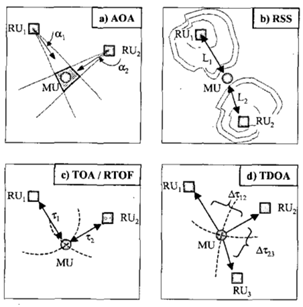
\includegraphics[scale = 0.4]{measurement}
\end{figure} 

In Angle-of-arrival (AOA) systems use directional antennas to measure the bearing and the angle to the points located at known positions are measured. The position value of device can be calculated with the intersection of several measurement, but the accuarcy is limited by shadowing and multipath reflections of radio signals \cite{20}. 

Received signal strength(RSS) systems calculate the distance value by taking the difference of the received signal power from the transmitted power. Some advanced propagation models are required to calculate the distance from the transmission loss in the air to eliminate the multipath fading and shadowing effects \cite{21}. 

Time based systems calculates the distance between measuring unit and signal transmitter with the help of propagation time like used in the global positioning systems generally. This process requires a perfect time synchronization between the mobile and stationary units \cite{20}.

In this thesis work, we implement a self positioning system in which every agent localize itself with the help of position beacons in the swarm with exactly known positions. The distance from the agents to these beacons in the swarm are assumed to be calculated with the help of a time of arrival(TOA) solution in which a node can calculate its distance to the transmitter beacon by measuring the difference between the timestamps of transmission and reception of the signal. 


\subsection{Trilateration Process} \label{Trilateration_Process_ref}

Trilateration process is used to determine the three dimensional position of unknown locations with the help of distance measurement to known positions \cite{22}. In self positioning systems, the main approach is to calculate the position of mobile agents with the help of distance measurements to the beacons with exactly known positions. This position calculations are handled with trilateration process. It is widely used in wireless sensor network topologies and local positioning systems.  In theory, it is needed to have at least four beacon nodes to calculte an unknown position in 3D, and at least three beacon nodes to calculate an unknown position in 2D environment. But these worst case numbers are generally not sufficient to estimate an unknown position with a good accuracy due to errors on range calculations and synchronization problems. Figure \ref{trilateration_ref} demonstrates a simple trilateration procees in 2D environment with the help of  three position beacons. Suppose a mobile device which tries to estimate its position with the help of local positioning system is at the red point in the figure. If it can measure its distance to the beacons named A,B and C with exactly known positions, it will be possible to estimate the unknown position of this mobile device with the same approach used in global positioning systems. 


\begin{figure}[H]
	\caption{Trilateration Process \cite{101}} \label{trilateration_ref}
	\centering
	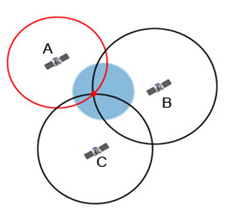
\includegraphics[scale = 1]{trilateration}
\end{figure}



\section{Formation Control Systems}
Formation control problem have different subproblems like formation shape generation, formation reconfiguration$\&$selection and formation tracking \cite{12}.  
In formation shape generation, agents are expected to get a formation shape which can be defined by external commands or with some mathematical constraint functions \cite{16}.  One general approach is to consider artificial potential functions. Samitha and Pubudu \cite{17} have presented an artificial potential function method  based on the consideration of the problem as controlling for the positioning of a swarm into a shape, bounded by a simple closed contour. This approach results in deploying uniformly of swarm agents within the contour.  Their work provides analysis about the stability and robustness of the proposed system based on Lyapunov like functions. Figure \ref{samitha_obstacle} illustrates a simulation environment of a swarm getting the desired pentagonal like formation shape in presence of obstacles. Here the desired formation shapes is defined with an analytical expression and individual control laws for agent are composed with artificial potential functions using this analytical expression. 

\begin{figure}[H]
	\caption{Motions and Formation of the Agents in Presence of Obstacles \cite{17}} \label{samitha_obstacle}
	\centering
	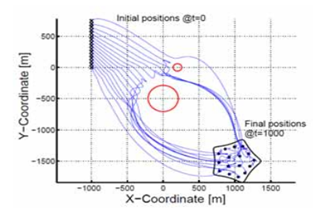
\includegraphics[scale = 0.7]{samitha}
\end{figure} 

In some applications, it may be needed to change the formation shape or splitting and joining of the agents together due to either a change in coordinated task requirements or change in environmental conditions such as narrow corridors. In such a scenario, the swarm has to propogate in a narrow corridor before reaching the desired goal state and it is not possible to follow this path by keeping the final desired formation shape. Hence, swarm has to adapt itself to environmental conditions while following a predetermined trajectory. This rask requires formation reconfiguration and dynamic task assignment of swarm agents to be dispatched. Hou and Slotine \cite{8} have defined a method based on global objective functions to provide formation control of a swarm agent. In their approach it is possible to implement scaling and rotating functions into control laws to adapt the swarm to environmental conditions while achieving a specific task. 

\begin{figure}[H]
	\caption{A Group of 100 Robots in a Rotating and Scaling Ellipse Formation \cite{8}} \label{slotine_fig_ref}
	\centering
	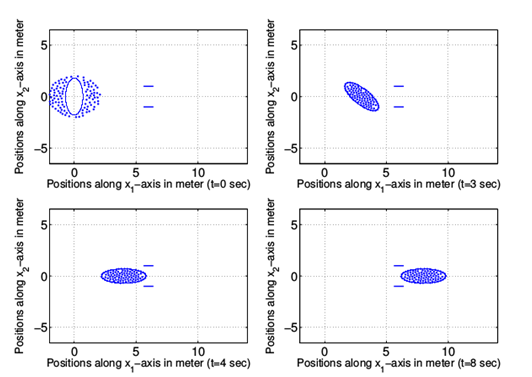
\includegraphics[scale = 1]{slotine}
\end{figure} 

Figure \ref{slotine_fig_ref} illustrates a simulation environment with a swarm of 100 mobile agents with an ellipsoidal formation shape. The formation shape is rotated dynamically to follow a path through a narrow corridor. Swarm has to adapt this  rotation maneuver to follow the desired trajectory. This kind of dynamical adaptations are always required in complex tasks in real time applications with complicated workspaces. 
One of the subproblems studied in formation control is formation tracking. The main objective of this problem is to maintain a desired formation with a group of robots, while tracking or following a reference trajectory. The solutions for the formation tracking approaches can be classified into three basic strategies as leader-following, virtual structure and behaviour based approaches \cite{12}. The most general strategy to provide a solution for this problem is leader-following swarm structures \cite{18}. Other strategies have a basis on optimization and graph theory approaches \cite{12}. Kumar, Fierro and Das proposed a vision based formation control framework  for this problem. This framework has a leader following infrastructure \cite{18}. Figure \ref{Kumar_Ferrro} illustrates a simulation environment of this leader follower approach on formation tracking problem. The individual agents achieve a coordinated turn by keeping their relative positions to their local neighbors. 

\begin{figure}[H]
	\caption{Five Robot Formation With Trajectory Tracking \cite{18}} \label{Kumar_Ferrro}
	\centering
	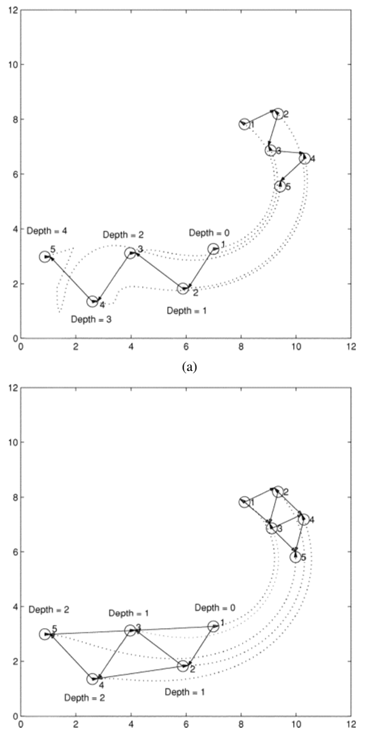
\includegraphics[scale = 0.65]{kumar}
\end{figure} 


In leader following strategy, some of the agents in the swarm are the leaders to manage the rest of the swarm to achieve a desired specific task and the rest of the agents act as followers. This approach reduces the formation control problem into tracking control problem of individuals to follow the leader from a desired distance and bearing angle, thus the stability and convergence analysis of the formation can be done with the usage of single tracking controllers of members thus simplifying the tracking problem of a network of agents to a single agent. Kumar, Fierro and Das at \cite{18} proposed a control framework in which follower agents move along a trajectory afterwords the leader agent with a desired separation distance $l_{ij}$ and desired relative bearing angle $\psi_{ij}$.  Figure \ref{leader_follower_ref} represents a formation control with three agents where R3 is the leader and R1,R2 are the follower agents. 

\begin{figure}[H]
	\caption{Leader-Follower Systems \cite{18}} \label{leader_follower_ref}
	\centering
	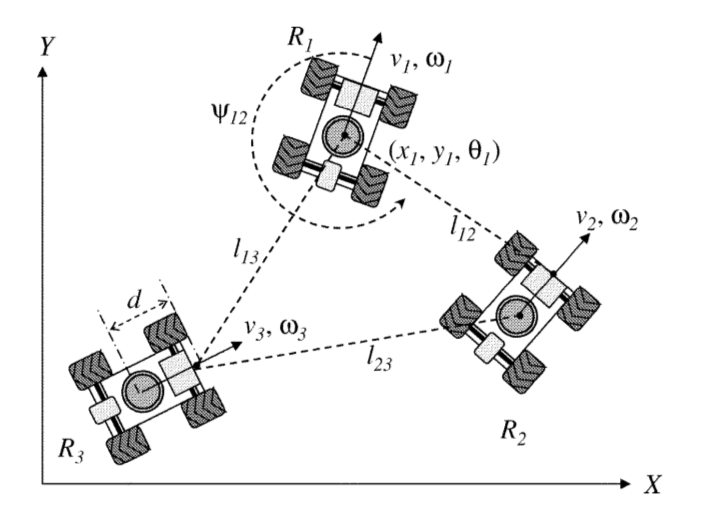
\includegraphics[scale = 0.5]{leader}
\end{figure}


In this approach it is hard to gather the agents in a certain shape. Another drawback is that, determining the separation and bearing angles for individual agents is getting harder as the number of agents in the swarm increases and this strategy is not fault tolerant to the absence of communication between agents.


In virtual structure approach, the formation is composed with a virtual rigid body. Formation control is applied to the whole virtual structure and then the individual agent control laws are determined with inverse dynamic solutions \cite{12}.  Lewis and Tan proposed a virtual structure based method for formation control in \cite{23} with a bidirectional flow control where robots move to stay in the virtual structure when the swarm is following a trajectory and virtual structure adapt itself to the robots' current positions to compensate the relative errors at the end of that maneuver. 

\begin{figure}[H]
	\caption{Maneuver of a Formation and Compensation of Virtual Structure}
	\centering
	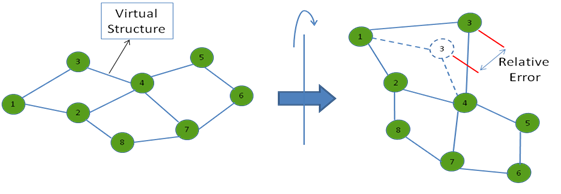
\includegraphics[scale = 0.95]{virtual_structure}
\end{figure}

In virtual structure strategy it is easy to achieve a coordinated behavior for the group to maintain the formation during a trajectory tracking or a maneuvering, but it is not a suitable strategy to apply a formation control to achieve certain geometrical shape with the swarm agents. 


Behavior based strategies model every agents' behaviors to achieve specific tasks with swarm. These behaviours may be very simple like randomly walk and avoidance of  obstacles in the environment or they may be defined in a very complicated manner in order to achieve complex formation shapes with the entire swarm while for example optimizing the overall energy consumption depending  upon the implementation of the controller structures.  One of the main usage of this strategy is artificial potential field based implementations . Cheng and Nagpal have introduced a robust and self repairing formation control method for swarms \cite{24}. In this approach, individual control laws for the agents are equipped with the artificial forces defined between agents themselves (to avoid collisions) and between the desired formation shape and agents. This solution provides robustness to the agent losses in the swarm during formation control and the rest of the swarm has the ability to refiil their absence in real time without changing the dynamics and the parameters of the formation controller. Because individual control laws are not dependent on the other member of the swarm. Each agent can calculate its own control input at an instant time with current formation shape and current members of the swarm and the whole swarm converge another equilibrium with current members \cite{24}. Figure \ref{izgara_ref} shows a simulation output of their work. Some of the agents from the right bottom corner of the desired formation shape are removed away from the swarm and the rest of the agents refill their absence during runtime. One of the main disadvantage of the artificial potential based approaches is that , the control forces applied to individual agents are determined instantaneously in accordance with that agent's and the other agents' positions and they cannot guarantee the optimization of the total distance travelled by the agents. Another drawback, related with this type of solution is that, there is a possibility to have local minimas in the solution where an agent reaches an undesired configuration point under the equilibrium of different types of artificial force components. In that case the total control input acting on the agent will be zero because of canceling force vectors which has opposite directions to each other generated by formation shape and obstacles etc. this strategy the solution may converge slowly to the steady state due to absence of generalized goal states for individual agents in the final state of formation. Because, there is no specific goal state for the individual agents to reach at the final configuration and they are expected to get a global equilibrium with the help of different artificial force components. 

\begin{figure}[H]
	\caption{Formation Control with Artificial Forces \cite{24}} \label{izgara_ref}
	\centering
	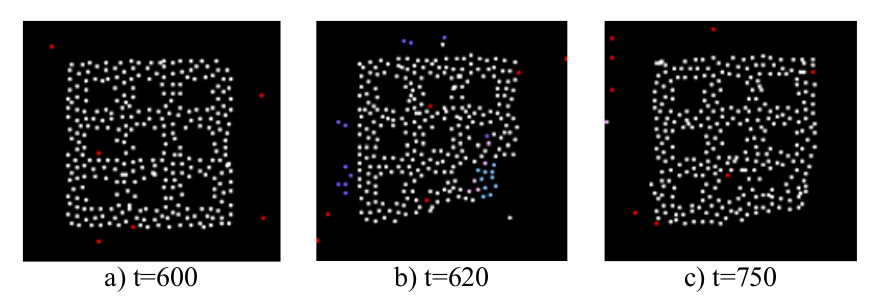
\includegraphics[scale = 0.4]{potential}
\end{figure}


Another approach is to define mathematical constraints and objective functions to achieve a specific formation shape by controlling the shape of the swarm colony while followinfg a trajectory.  Kumar and Belta \cite{25} presented an abstraction method of configuration space to a manifold defined as $A  = G x S$ where $G$ is a Lie group representing the position and the orientation of the swarm  and S represents the shape of the manifold.  They provide individual control laws which can be separately handled to manipulate the lie group $G$ to achieve formation tracking and orientation control and to manipulate the shape $S$ to achieve different geometrical shapes.Their method define the desired formation shape with shape manifold equations and control the orientation and the scale of this shape with lie group. Figure \ref{kumar_belta}
shows a simulation output in which the shape is defined as a rectangular area. The orientation and the scaling of the formation shape is dynamically changed to adapt the swarm different environmental conditions.Cheah and Slotine \cite{8} proposed a method based on objective functions . Common drawback for these researches, they can only implement a limited number of simple geometrical shapes because the desired formation shapes must be analytically identified on order to compose the related objective functions or shape manifolds. Even if it is possible to define a simple geometrical shape and to control the rotation and the scaling of this shape dynamically, there may be need for more complex and dynamically changing formation shapes rather than scaling and rotation maneuvers in real time applications. 



\begin{figure}[H]
	\caption{Formation Control with Objective Functions \cite{25}} \label{kumar_belta}
	\centering
	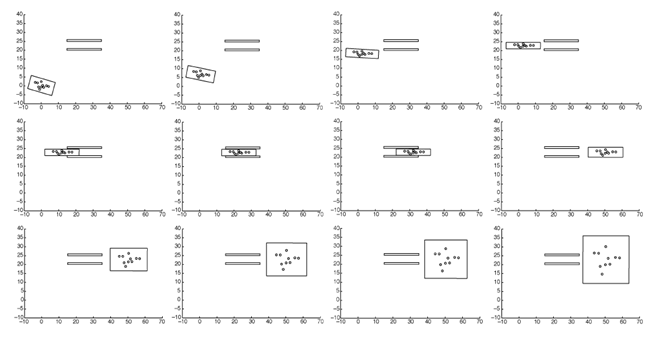
\includegraphics[scale = 0.8]{manifold}
\end{figure}



\section{Partitioning Complex Geometrical Shapes}

In this thesis work, one of the proposed solutions for the formation control problem is to partition the desired complex shapes into subsets of goal states for each type of agent in the swarm. Main idea is to dynamically assign the agents to these goal states on runtime to minimize the overall displacement of the swarm. Shape partitioning process is used to determine the goal states of the agents within the formation to cover the desired complex geometrical shape. There are some different solutions in the literature including fractal filling of space algorithms, bubble$\&$circle packing algorithms and advancing front algorithms. 

Fractals are self similar  patterns in all scales of themselves. They are defined with simple rules and they can cover any complex shape in the nature by progressing this simple rules iteratively. This approach is widely used in mesh generating algorithms and filling space problems.  Shier and Bourke \cite{26} have introduced a randomized fractal filling of space algorithm. They proposed a fractal based method to cover a given geometrical shape with the desired shapes and they provide the proof of their algorithm is space-filling with the following equations. Let $A$ be the total area to be filled. In our case, $A$ will be the area of the desired formation shape. If we choose the area of the fractals sequentially (i.e. bubbles which are representing the coverage area of the agents)  while filling the desired formation shape as $A_i$ with the following equation

	\begin{equation} \label{A_i_func}
	A_i = {\frac{A}{{\zeta(c,N)(i+N)^c}}}
	\end{equation}	
	
	where ${\zeta(c,N)}$ is the Hurwitz zeta function defined by 
	\begin{equation} \label{hurwitz}
	\zeta(c,N) = \sum_{i=0}^{\infty}\left(\frac{1}{(i+N)^c}\right)
	\end{equation}
	This Hurwitz zeta function will converge to zero while $i\to\infty$  with selection of $c>1$ and $N>0$. In view of Equation \ref{A_i_func} one can write by replacing the Hurwitz zeta function with the definition given in Equation \ref{hurwitz}
	\begin{equation} \label{A_i_equation}
	\sum_{i=0}^{\infty}A_i = \sum_{i = 0}^{\infty}\left(\frac{A}{\zeta(c,N)(i+N)^c}\right) = A
	\end{equation}


such that the sum of all areas $A_i$ is the total area $A$ to be filled, that is, if the algorithm does not halt then it is space-filling. Thus, it is possible to fill the desired shape with fractals chosen with areas defined in Equation \ref{A_i_equation}. Some of the outputs of their algorithm is given at Figure \ref{space_filling}. The desired shapes are filled with rectangular and star shaped fractals by selecting the areas as described in Equation \ref{A_i_equation}.



\begin{figure}[H]
	\caption{Space Filling Examples with Randomized Fractals \cite{26}} \label{space_filling}
	\centering
	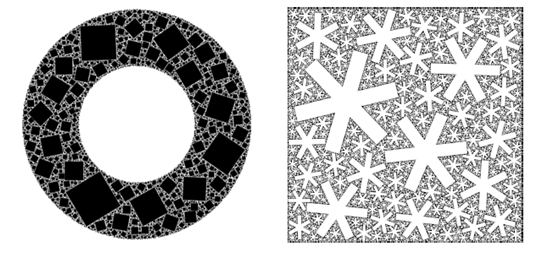
\includegraphics[scale = 1]{randomized1}
\end{figure}


Bubble$\&$Circle packing algorithms are widely used for mesh generation problems in finite element method. Shimada and Gossard \cite{27} proposed a method based on interbubble forces to provide close packaging of bubbles in desired geometrical shape. They define artificial interbubble forces to avoid collisions between bubbles and shape forces to keep the bubbles at the interior region of the desired shape. This idea is similar to the potential field based approaches in formation control problem since they both define artificial force components on individuals to cover a desired shape homogenously. The related interbubble forces are described at Figure \ref{interbubble_ref}. These forces have a nonlinear function of distance between the center of each bubbles and if this distance is larger than $l_o$, the interbubble forces are negative which means they attract each bubble towards the other ones. Interbubble forces increase while the distance between bubbles are decreasing to provide collision avoidance between bubbles. $l_o$ is the stable distance in which there is no interbubble force acting on bubble and it reaches an equilibrium point in the workspace.

\begin{figure}[H]
	\caption{Interbubble Forces \cite{27}} \label{interbubble_ref}
	\centering
	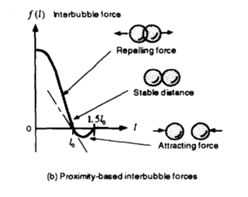
\includegraphics[scale = 0.3]{interbubble}
\end{figure}

The main idea is provide a close packing of bubbles which mimics a pattern of Voroni tessellation, corresponding to well shaped Delaunay triangles or tetrahedras.Figure \ref{tetrahedra} shows the corresponding voronoi polygons and delaunay triangles of a set of packed bubbles. The center of the cells in voronoi polygons are selected as the centers of the bubbles. Delaunay triangles corresponding to the set of uniformly packed of bubbles are well-shaped triangles \cite{27}. 

\begin{figure}[H]
	\caption{Uniform and Non-Uniform Node Spacing \cite{27}} \label{tetrahedra}
	\centering
	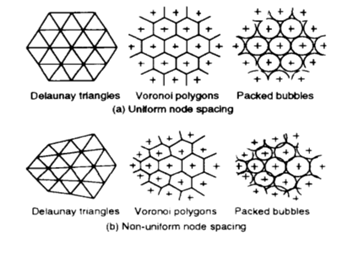
\includegraphics[scale = 0.35]{nodespacing}
\end{figure}

With the help of these interbubble forces, they provide an adaptive bubble packing algorithm for mesh generation. A result with a 2D shape is given at Figure \ref{mesh_genearation_ref}. At the end of 50 iterations, bubbles cover the desired shape with uniform spacing with the help of interbubble forces and the resultant delaunay triangulation corresponding to the set of packed bubbles are well-shaped triangles. 


\begin{figure}[H]
	\caption{Mesh Generation with Interbubble Forces \cite{27}} \label{mesh_genearation_ref}
	\centering
	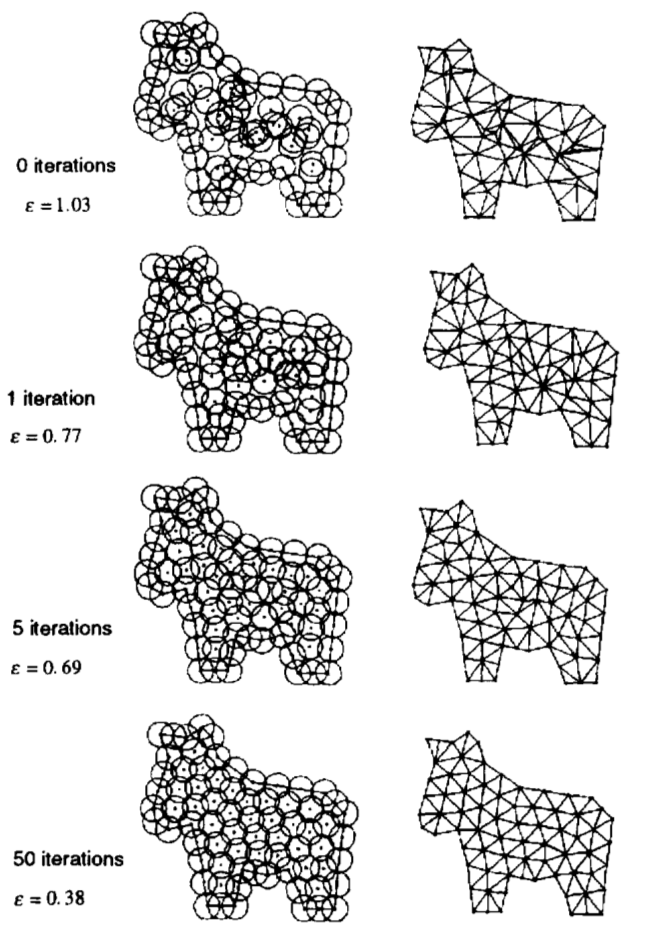
\includegraphics[scale = 0.4]{interbubble2}
\end{figure}

This approach can easily be augmented for different types and number of shapes to partition a complex geometrical shape with regular sets. It is possible to generate a mesh with different shapes which represents different types of agents in the swarm, rather than using bubbles with same radius. With this adaptation on the proposed method, it is possible to partition the desired shape into goal states which are subsets of different types of agents in the swarm with the help of interbubble forces. 

Advancing front methods are one of the alternatives used in mesh generation in literature.  In a two dimensional advancing front method, new triangles are added into the domain from the initial front boundary and the front is propogated iteratively between the meshed and the unmeshed region. The initial front is created by the desired outer boundary of the shape and the procedure continues until the given domain is fully meshed. 


\begin{figure}[H]
	\caption{Triangulation with Advancing Front Method \cite{103}}
	\centering
	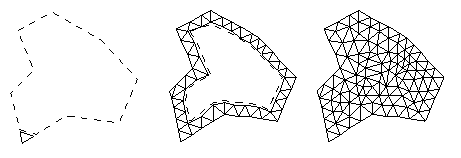
\includegraphics[scale = 0.65]{advancing}
\end{figure}


% CHAPTER 3

\chapter{METHODOLOGY}
\label{chp:Methodology}


\externaldocument{chapter1}
\externaldocument{chapter2}
\externaldocument{chapter6}
\externaldocument{chapter4}
\externaldocument{chapter5}

In this thesis work, the problem of dynamical formation control of heterogeneous mobile robots is reduced down to two subproblems such as local positioning and formation control.  In our implementation there are two main types of agents in the swarm. First type agents have position measurement sensors on their boards. We call these agents position beacons and only limited number of agents are position beacons in our swarm. Second type agents do not have position sensors on their boards. Local positioning subsystem proposes a solution for the localization of agents in the workspace for second type of agents. On the other hand, formation control subsystem implements algorithms to cover the desired formation shape homogeneously with the agents in the swarm. In this chapter, our solutions for these subproblems are presented in details.

A general block diagram of the system design is illustrated in Figure \ref{general_system}. According to this diagram, local positioning system provides a basis for the formation control problem with agents' state vectors composed of translational positions and velocities. Basically, this subsystem provides position and velocity data to the second type of agents in the swarm. Formation control subsystem proposes a solution to achieve desired complex shapes with heterogeneous agents in the swarm. Formation control system gets the requested formation shape externally and creates individual control laws for agents to cover the desired shape homogenously. The implementation details of these subsystems are given in the following sections. 
\begin{figure}[H]
\caption{General Block Diagram of the Provided Solution} \label{general_system}
\centering
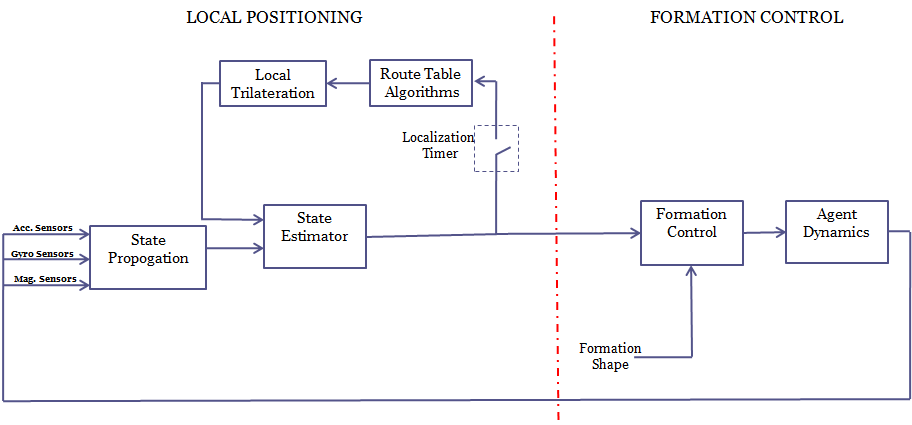
\includegraphics[scale = 0.58]{general_scheme}
\end{figure}

\section{LOCAL POSITIONING SYSTEMS} \label{LOCAL POSITIONING SYSTEMS_ref}
Local positioning system is a subsystem to provide a complete solution to the localization of the second type agents in the workspace. As discussed in Section \ref{Objectives}, agents are expected to have low sensor capabilities and only a limited number of them have external position measurement sensors on their boards and we call these agents position beacons in our project. The rest of the swarm which is composed of second type agents, has to maintain their position$\&$velocity data with the help of their inertial measurements and local trilateration process. Propagation of the states with these inertial measurements are always inclined to drift problems due to the error$\&$noise and bias problems of the sensors \cite{91}. Because of this problem, we have corrected these state vectors with an external measurement provided by local trilateration process. We have proposed a complete solution for this subsystem as illustrated in Figure \ref{figure_lps}.

\begin{figure}[H]
\caption{Local Positioning System} \label{figure_lps}
\centering
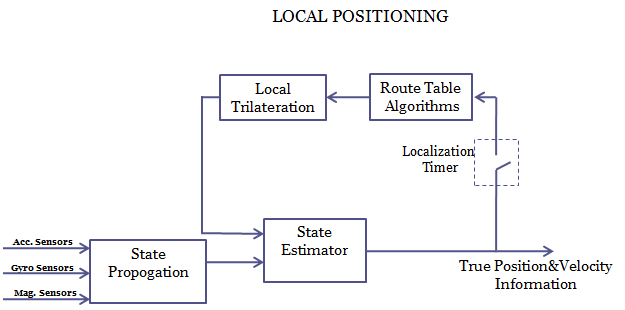
\includegraphics[scale = 0.65]{lps}
\end{figure}

As illustrated in Figure \ref{figure_lps}, agents propagate their states with the help of inertial measurements. This state propagation process is executed with high speed data provided by the inertial sensors. On the other hand, trilateration and route table determination processes require iterative and time consuming algorithms and their implementation details are given in the following sections. It is not possible to execute the trilateration and route table determination algorithms with the same execution frequency of state propagation process. Because of this reason, a localization timer to provide the minimum required time for the route table determination and trilateration process is implemented to the solution. Agents will correct their state vectors with the localization period by measuring their positions with trilateration process and execute the update procedure in their state estimator algorithms. The requirement about the maximum value of the localization period is determined with the help of Monte Carlo simulations discussed in Section \ref{lps_ref} by defining a maximum allowable error on the position data. 

Local trilateration process requires distance measurements to the position beacons which are direct neighbors of an agent. Route table algorithms are used to provide information to the agents about the position beacons whether they are direct neighbors or not. On the other hand, route tables also implement a mesh network between agents. This network is used to transport data globally over the network. It is composed with a bidirectional graph in which each agent can communicate with its direct neighbors. In this graph, we have assigned an edge between two nodes if there is a radio link between them. This line of sight(LOS) radio link is the main criteria for the agents to become direct neighbors in the network. Thus, having a physical Euclidian distance to an agent within the communication range is not enough to be the direct neighbor with that agent, i.e. even if two agents are very close to each other in the workspace, they are not direct neighbors if there is no radio link between them because of an obstacle preventing the line of sight. Figure \ref{sample_mesh} shows an example of a mesh network created with 8 agents in the environment.

\begin{figure}[H]
\caption{A Sample Mesh Network Created with 8 Agents} \label{sample_mesh}
\centering
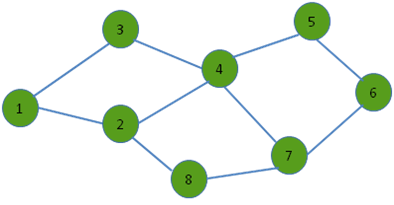
\includegraphics[scale = 0.58]{mesh}
\end{figure}
 
\subsection{Local Trilateration Process}
Trilateration process helps the second type agents to localize themselves with the help of position beacons which are their direct neighbors.  Trilateration calculations use distance measurements to the position beacons with known positions, to determine the coordinates of second type agents \cite{22}. These measurements are assumed to be done with the help of time of arrival(TOA) methods as discussed in Section \ref{sssec:num1}. In a TOA solution, an agent is able to measure the distance from itself to a position beacon only if it is a direct neighbor of that position beacon. Figure \ref{beacons_ref} illustrates simulation environment of a swarm which includes 5 position beacons. Here agent $C$ tries to localize itself with the help of distance measurements $r_i$ and the position data $B_i$ of the position beacons. It has 4 position beacons as direct neighbors in the network and this information is provided by the route table of agent $C$ as defined in Section \ref{route_route}.

\begin{figure}[H] 
\caption{Environment for Trilateration Process} \label{tri_late}
\centering
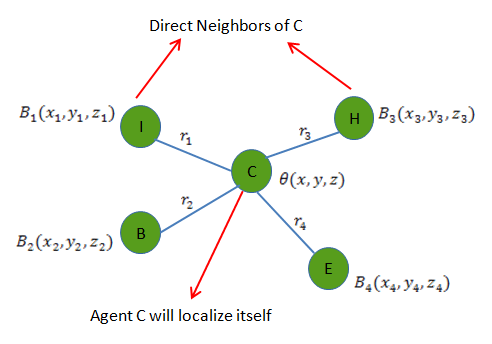
\includegraphics[scale = 0.55]{beacons}
\label{beacons_ref}
\end{figure}

For the simulation environment illustrated in Figure \ref{tri_late}, the distance function to any position beacon can be written as follows \cite{22};

\begin{equation} % eq 2
{r_i} = \sqrt{(x-x_i)^2 + (y-y_i)^2+ (z-z_i)^2}    \hspace{0.3cm}   (i=1,2,...,n)
\end{equation}

where $i$ denotes the beacon number and $n$ is the total number of position beacons which is equal to 4 in our case.  In general, we have $n$ number of constraints in the solution of the localization problem. These constraints are defined as spherical functions for a localization problem in 3 dimensional workspace \cite{22}. In our work, we have implemented a two dimensional localization solution with the assumption of each agent of the swarm conserve the same vertical position within the Earth centered coordinate system. With this assumption, the problem for the localization process has constraints with circle functions rather than spherical ones, presented with

\begin{equation}
(x-x_i)^2 + (y - y_i)^2 = {r_i}^2 \hspace{0.3cm}   (i=1,2,...,n)
\end{equation}

It is possible to use these $n$ circular constraints to calculate the unknown position of the agent $C$. For this purpose, lets assume $\theta = (x,y)$ is representing the coordinates of agent $C$ and $B_1 = (x_1,y_1) ; B_2 = (x_2,y_2) ; B_3 = (x_3,y_3) ; ...  ; B_i = (x_i,y_i)$ are the measured positions of the position beacons.

If any of these beacons is considered as the reference beacon and named with an index of $r$, the distance equations can be provided as following:

The distance between the agent $C$ and any beacon $i$ represented as

\begin{equation} \label{3.3}
d_i(\theta) = \sqrt{\left((x - x_i)^2 + (y - y_i)^2\right)}
\end{equation}

The distance between the reference beacon which is located at $B_r = (x_r,y_r)$ and the other beacons is evaluated as

\begin{equation}
d_{ir}(\theta) = \sqrt{\left((x_i - x_r)^2 + (y_i - y_r)^2\right)}
\end{equation}

The distance between the agent $C$ and the reference beacon is obtained as

\begin{equation}
d_r(\theta) = \sqrt{\left((x - x_r)^2 + (y - y_r)^2\right)}
\end{equation}

Adding and subtracting $x_r, y_r$ and $z_r$ in equation \ref{3.3} gives

\begin{align} \label{tri_expressi}
\begin{split}
d_i^2(\theta) = & (x - x_r + x_r - x_i)^2 + (y - y_r + y_r - y_i)^2 \\ 
              = & (x - x_r)^2 + 2(x_r - x_i)(x - x_r) + (x_r-x_i)^2 \\
              + & (y - y_r)^2 + 2(y_r - y_i)(y - y_r) + (y_r - y_i)^2
\end{split}
\end{align}

Replacing the expressions in equation \ref{tri_expressi} by $d_{ir}$ and $d_r$, the equation can be written as:

\begin{equation}
 2((x_i - x_r)(x - x_r) + (y_i - y_r)(y - y_r)) = d_r^2(\theta) + d_{ir}^2 - d_i^2(\theta)
\end{equation}

this general expression is valid for each beacon with $i$ changing from $2$ to $n$ (by assuming that we have chosen the first position beacon with $"r=1"$ as reference beacon)

\begin{align}
\begin{split}
& (x_2 - x_1)(x - x_1) + (y_2 - y_1)(y - y_1) = \frac{1}{2} [d_1^2(\theta) + d_{21}^2 - d_2^2(\theta)] \\
& (x_3 - x_1)(x - x_1) + (y_3 - y_1)(y - y_1) = \frac{1}{2} [d_1^2(\theta) + d_{31}^2 - d_3^2(\theta)] \\
& ... \\
& (x_n - x_1)(x - x_1) + (y_n - y_1)(y - y_1) = \frac{1}{2} [d_1^2(\theta) + d_{n1}^2 - d_n^2(\theta)]
\end{split}
\end{align}

if $b_{ir}$ is defined for each beacon as follows:

\begin{equation}
b_{ir} := \frac{1}{2}[d_r^2(\theta) + d_{ir}^2 - d_i^2(\theta)]
\end{equation}

then the linearized system equations can be represented with $A\vec{x} = \vec{b}$ type equation where;

\begin{equation}
A = \begin{bmatrix}
x_2 - x_1 & y_2 - y_1\\
x_3 - x_1 & y_3 - y_1\\
...       & ...      \\
x_n - x_1 & y_n - y_1\\
\end{bmatrix}				
\end{equation}

\begin{equation}
x = \begin{bmatrix}
x - x_1\\
y - y_1\\
\end{bmatrix}
\end{equation}

\begin{equation}
b = \begin{bmatrix}
b_{21}\\
b_{31}\\
... \\
b_{n1}\\
\end{bmatrix}
\end{equation}

with $A$ is a $(n-1)\ x\ 2$ matrix and $b$ is a $(n-1)\ x\ 1$ vector.

There are some possible solutions to this type of equation regarding with the structure of matrix $A$ and vector $b$.\\

\underline {\textit{Solution to $A\vec{x} = \vec{b}$ Problem}}\\
In a localization problem handled in two dimensional space, the $A$ matrix has $(n-1)$ rows and $2$ columns, where $n$ is the number of position beacons which are direct neighbors of an agent. There is no solution when the number of neighbors lower than $3$ (i.e. $n<3$) \cite{22}. When the number of neighbor position beacons are equal or greater than $3$ we have three different solutions according to the structure of the linearized equations.

\textit{1) Unique Solution:}\\
 If A is a $2\ x\ 2$ matrix (i.e. $n=3$) and the its rank is $2$, then the solution of $\vec{x}$ is unique with \cite{linear_ders_notu}

\begin{equation}
\vec{x} = A^{-1}\vec{b}
\end{equation}

where $\vec{x}$ is the unique solution. \\
  
\textit{ 2) Minimum Norm Solution With Pseudo Inverse:} \\  
If $A$ is a $(n-1)\ x\ 2$ dimensional matrix where $n>3$ ,which means the number of neighboring position beacons greater than $3$, and if columns of $A$ matrix form a linearly independent set (full column rank matrix) then the solution can be found with the projection of $\vec{b}$ over range space of $A$, $Proj_{R(A)}\vec{b}$ where \cite{linear_ders_notu}

\begin{equation}
Proj_{R(A)}\vec{b} = A (A^TA)^{-1}A^T\vec{b}
\end{equation}

\begin{align}
\begin{split}
& A\hat{x} = Proj_{R(A)}\vec{b}\\
& A\hat{x} = A(A^TA)^{-1}A^T\vec{b}
\end{split}
\end{align}
 
We can justify this expression by passing the righthand side term to the left

\begin{equation}
 A(\hat{x} - (A^TA)^{-1}A^T\vec{b}) = 0
\end{equation}

then 

\begin{equation}
\hat{x} = (A^TA)^{-1}A^T\vec{b}
\end{equation}
  
$(A^TA)$ is invertible since $A$ matrix is full column rank matrix, so 

\begin{align}
\begin{split}
\mathcal{N}(\mathbf{A}) = \{0\} \hspace{0.3cm}  and  \hspace{0.3cm}  \mathcal{N}(\mathbf{A})^\perp =\mathbb{R} ^n 
\end{split}
\end{align}
  
then 
  
\begin{equation}
Proj_{ \mathcal{N}(\mathbf{A})^\perp}\hat{x} = \hat{x}
\end{equation}
  
this concludes that $\hat{x}$ is the unique minimum norm solution to the $A\vec{x} = \vec{b}$ problem\\
	
	
\textit{3) Minimum Norm Solution with Newton Iteration Method}\\	
If matrix $A$ has the dimensions of $2\ x\ 2$ or $(n-1)\ x\ 2$ with $n>3$ and if rank of $A$ matrix is equal to $1$ then the solution to the $A\hat{x} = \vec{b}$ problem can be found iteratively with the help of nonlinear least squares method that minimizes the cost function which is defined as sum of squares of the distance errors \cite{22} :
	
\begin{equation} \label{cost_func_tri}
F(\theta) = \sum_{i=1}^{n} \left(f_i^2(x,y)\right)
\end{equation}
	
with
	
\begin{equation}
f_i(x,y) = \sqrt{(x-x_i)^2 + (y - y_i)^2} - r_i = f_i(\theta) 
\end{equation}

where $r_i$ is the measured distance to a position beacon $i$ and $(x_i, y_i)$ is calculated position data of agent $C$ iteratively.

There are various algorithms to minimize the cost functions in the literature. We have used Newton iteration to find the optimal solution in this thesis work. Because convergence of this method is quadratic in general and the performance of the algorithm is extremely increased by choosing proper initial conditions \cite{wiki_newton}. We have used the propagated position data as an initial condition for the optimization process to make the algorithm terminated very fast with correct results. Algorithm is implemented as follows:

Considering  $f(\theta)$ as

\begin{equation}
f(\theta) = \begin{bmatrix}
f_1(\theta) \\
f_2(\theta) \\
...         \\
f_n(\theta)
\end{bmatrix}
\end{equation}


We have defined the Jacobien matrix as follows:

\begin{equation}
J(\theta) = \begin{bmatrix}
\frac{\partial{f_1(\theta)}}{\partial{x}} & \frac{\partial{f_1(\theta)}}{\partial{y}} \\
\frac{\partial{f_2(\theta)}}{\partial{x}} & \frac{\partial{f_2(\theta)}}{\partial{y}} \\
... & ... \\
\frac{\partial{f_n(\theta)}}{\partial{x}} & \frac{\partial{f_n(\theta)}}{\partial{y}} \\
\end{bmatrix}
\end{equation}

	
Suppose we are trying to find the position of an agent defined with the vector of $\vec{R}$	
\begin{equation}
 \vec{R} = \left(\begin{matrix}
  x \\ y 
 \end{matrix}\right)
\end{equation}

To optimize the cost function, Newton iteration is implemented as follows;

\begin{equation}
 \vec{R}_{\{k+1\}} =  \vec{R}_{\{k\}} - (J^T_{\{k\}}J_{\{k\}})^{-1}J^T_{\{k\}}\vec{f}_{\{k\}}
\end{equation}	

where $\vec{R}_{\{k\}}$, $J_{\{k\}}$ and $\vec{f}_{\{k\}}$ denotes the variables calculated at $k^{th}$ iteration. The explicit form of the equations can be derived as follows;
	
\begin{equation}
J^TJ = \left(\begin{matrix}
\sum_{i=1}^{n} \frac{(x-x_i)^2}{(f_i+r_i)^2} &  \sum_{i=1}^{n} \frac{(x-x_i)(y-y_i)}{(f_i+r_i)^2} \\
\sum_{i=1}^{n} \frac{(x-x_i)(y-y_i)}{(f_i+r_i)^2} &  \sum_{i=1}^{n} \frac{(y-y_i)^2}{(f_i+r_i)^2}
\end{matrix}\right)
\end{equation}	

and 

\begin{equation}
J^T\vec{f} = \left(\begin{matrix}
\sum_{i=1}^{n}\frac{(x-x_i)f_i}{(f_i+r_i)} \\
\sum_{i=1}^{n}\frac{(y-y_i)f_i}{(f_i+r_i)}
\end{matrix}\right)
\end{equation}
	
	
\subsection{Route Table Determination} \label{route_route}
We have implemented a localization solution in which each second type agent is getting in trilateration process with the position beacons in the swarm as we have introduced previously. It is needed to be direct neighbors of the position beacons to get in trilateration process. In our project, route tables are used to provide information to the agents about the position beacons whether they are direct neighbors or not. On the other hand, they are used to create a mesh network in the swarm to provide a communication backbone. With this mesh network it is possible to send any data globally over the network to any destination by using agents as relays to transmit the data. In our implementation, each agent had its own route table in the network. These route tables include the information about the next nodes and costs to any destination in the network. Next nodes are representing the node which the data will be transferred next for that destination and costs are representing the minimum number of hops (i.e. number of relay agents on the path) for that destination. We have used the cost information for the position beacon destinations to check whether the agent is direct neighbor of that position beacon or not. In other words, the cost to a position beacon is equal to 1 in the route table, if that agent is the direct neighbor of the position beacon


	
\subsubsection{Routing Algorithm- Bellman Ford}
As mentioned in the Section \ref{Objectives}, agents are assumed to have a limited communication range and bandwidth and the communication topology in the swarm must be implemented with a wireless mesh network. In this type of topology, each agent is a relay in the network and the data is transferred to the related destination with the help of route tables. This makes it possible to have the capability of transferring low bandwidth data through the network with multiple hops.  In this work, we have implemented this topology with a table driven routing scheme known as Bellman Ford algorithm. Bellman Ford is an algorithm that computes the shortest paths between any two node in a weighted graph \cite{wiki_bellman}. It has a drawback related with the routing loop problem which occurs in an event of one or more nodes in the graph are lost during the process. The probability of vanishing vertices during the execution of the algorithm is very high since the agents in the swarm have a small range of communication and have a great possibility to lose their connection with the rest of the swarm. For this reason we have implemented an extension of the Bellman Ford algorithm known as Destination-Sequenced Distance Vector Routing Protocol(DSDV) algorithm.  
	
\begin{figure}[H]
\caption{Costs for Shortest Paths to Each Nodes from Agent 'B'} \label{bellman_ref}
\centering
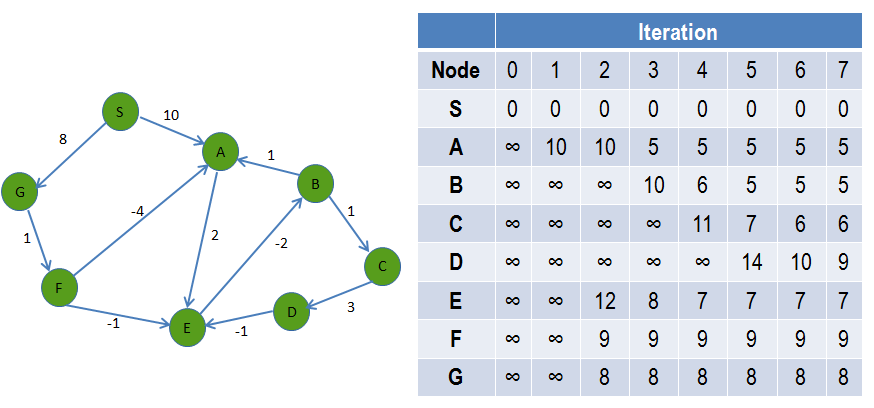
\includegraphics[scale = 0.50]{bellman}
\end{figure}

A simulation of the DSDV algorithm with a simple robot network in our problem is given in the Figure \ref{bellman_ref}. The algorithm to calculate the shortest paths from agent `B` to each destination on network, terminates at the end of 3 iterations. At the beginning of the process, the costs for each destinations are determined as infinitive. Then the shortest paths to the each agent in the given bidirectional graph are determined iteratively with the help of the DSDV algorithm. Since we have defined the shortest paths with the number of hops to each destination, we have used unit weight for each edge in the graph representing the cost of each hop while getting the related destination in the network is equal to 1. 

We have implemented DSDV algorithm to solve the routing problem in the mesh network. Figure \ref{routing_problem2} shows a simulation output illustrating routing loop problem.

\begin{figure}[H] 
\caption{Routing Problem Engaged by a Lost of a Node in Network} \label{routing_problem2}
\centering
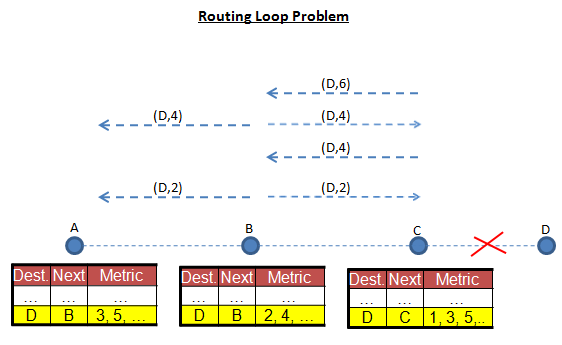
\includegraphics[scale = 0.65]{routing_problem}
\end{figure}

Suppose that agent D has lost its contact with the network due to some malfunction or by being lost wandering outside of the communication range of its closest neighbor. Before this event, agent C had a unit distance to agent D and consequently agent B had a 2 unit distance to agent D , agent A had a 3 unit distance to agent D. In case of a failure of agent D, on the next iteration, C updates its route table with 3 unit distance to agent D by taking as reference the agent B. Then agent B updates its route table with the shortest distance of 4 units to agent D\ referencing to agent C. This process diverges to infinity on the shortest paths with the increasing number of iterations. To provide a solution for this routing loop problem, DSDV algorithm implements the destination sequence numbers into the route tables of the nodes. A simulation output showing the route table for a node in a robot network is given in Figure \ref{dest_seq_ref}

\begin{figure}[H]
\caption{Route Table for Agent B in Robot Network} \label{dest_seq_ref}
\centering
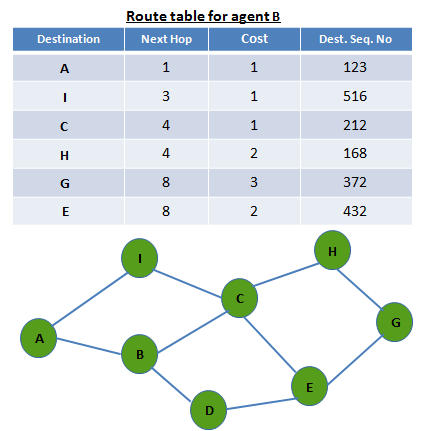
\includegraphics[scale = 0.75]{dest_seq}
\end{figure}

In the DSDV algorithm, each node transmits the updates in its own sequence number and routing table. In the network, when two routes to the same destination are received from two different neighbors, the algorithm executes the following rules;\newline
	- Choose the node with the larger destination sequence number \newline
	- If the sequence numbers are equal, then choose the route with minimum number of hops and update the route table.

In Figure \ref{dest_seq_ref}, node B has destination sequence numbers to each destination in its route table. These numbers are used to update the network with the rules defined above, in the case of link addition and link brakes defined in following sections.
\newpage	
\subsubsection{DSDV Link addition}

Figure \ref{linkk_addition} shows a sample link addition condition to the robot network. In this example, robot A joins the network by creating a radio link with robot B. When a new node A joins the network, it transmits of its own route table including the destination to itself $<A,A,0,101>$. Then the following procedure will be handled during iterations; \newline
	-Node B receives the the transmission of A and inserts a new line into its route table with $<A,A,1,101>$ and propagates this new node to its neighbors \newline
	-Node C and Node D receives this transmission and inserts the new route to their route tables with $<A,B,2,101>$

\begin{figure}[H]
\caption{An Example for Route Table} \label{linkk_addition}
\centering
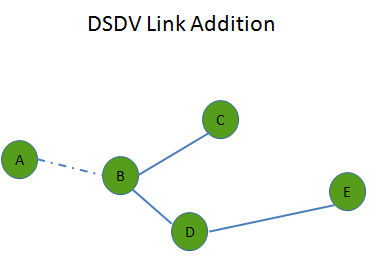
\includegraphics[scale = 0.65]{link_add}
\end{figure}	
		
\subsubsection{DSDV link breaks}

Figure \ref{linkk_brake} shows a sample link brake condition to the robot network. Robot B lost its connection with robot D. When the link between B and D breaks, node B gets no transmission from the D and notices the link breaks, then the following procedure will be handled; \newline
	- Node B update the cost for node D and E destinations to the infinity and increments the sequence numbers to these routes \newline
	- Node B propagates the updates to its neighbors and node A and node C updates the lines of the routes to the D and E, since the message from B includes higher sequence numbers for those routes.
		
\begin{figure}[H]
\caption{An Example for Route Table} \label{linkk_brake}
\centering
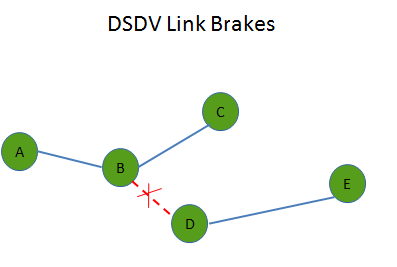
\includegraphics[scale = 0.65]{link_break}
\end{figure}
	
\subsection{Handling Lost Agents} \label{LostAgents}
The minimum number of position beacons required for the trilateration process is three for a two dimensional localization problem as illustrated in Section \ref{Trilateration_Process_ref} . Since the agents are assumed to have a narrow communication range, it is possible to not to find three  position beacons as direct neighbors for any agent at an instant time. In this case, it will not be possible to relocate these agents with trilateration and the position$\&$velocity data will drift from the real values with the increasing time passed without trilaterions. It is important to have a solution for this problem to keep the swarm together and to increase the robustness of the system against different environmental conditions. In our algorithm, concept of `Lost` agents and the procedures for these type of agents are described as follows:
	
	* An agent gets into 'Lost' mode, if it doesn't find at least three direct neighbors of position beacons at an instant time \newline
	* If an agent is in 'Lost' mode and missed the localization process for three times, it will get into 'Return to Home' mode \newline
	* If an agent is in 'Return to Home' mode, it will directly try to reach to the center of the desired formation shape.
		
The idea behind the 'Return to Home' mode is basically to increase the possibility of finding position beacons which are direct neighbors of the lost agent by directing it to the center of the swarm. A simple demonstration of this procedure is illustrated in Figure \ref{return_home_ref}
	
\begin{figure}[H]
\caption{Return to Home Approach of a Lost Agent} \label{return_home_ref}
\centering
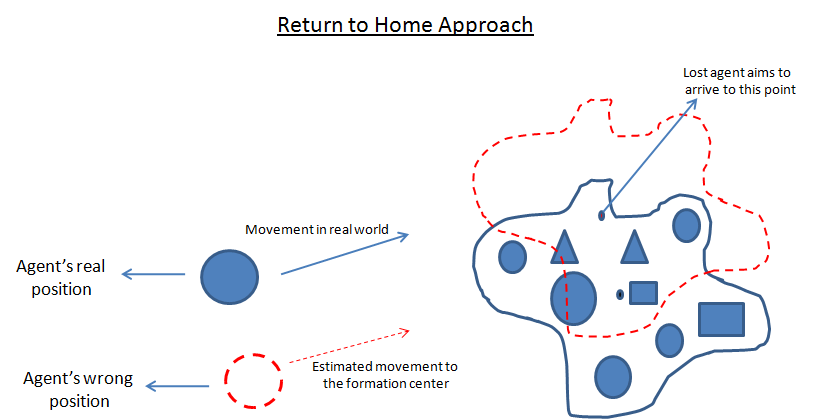
\includegraphics[scale = 0.60]{return_home}
\end{figure}
	
The lost agent aims to reach to the center of the formation and due to the errors on its position$\&$velocity data, it is expected to arrive to the red point illustrated in the figure. With this maneuver, the lost agent still have a chance to meet some position beacons in the swarm even if it directs itself to an incorrect goal state.
	
\subsection{State Estimation Procedure} \label{StateEstimationref}
In local positioning subsystem, second type agents are expected to execute a state estimator algorithm in which they propagate their state vectors composed of translational position and velocities with the help of inertial measurements. As discussed at the introduction of Section \ref{LOCAL POSITIONING SYSTEMS_ref} agents will update and correct their positions with the measurements provided by the trilateration process execeuted with the localization timer period. A Kalman estimator algorithm which uses the trilateration outputs as external measurements and the inertial measurements as inputs, is designed to fuse the inertial measurements with the trilateration calculations. The model for this observer system is defined as follows:
	
The state vector for each agent is defined as:

\begin{equation}
x_k = \begin{bmatrix}
X_k \\
\dot{X}_k\\
\end{bmatrix}
\end{equation}
	
where $X_k$ is the position and $\dot{X}_k$ is the velocity of the agents in x coordinates in two dimensional environment. All of the following procedures will be handled exactly the same for the state vector defined in y coordinates.

The discrete linear model is defined with the state equation of \cite{wiki_kalman}:

\begin{equation}
x_{k+1} = F_k     x_{k} + B_ku_k + w_k
\end{equation}
	
where $w_k$ is the process noise and 
\begin{equation}
F = \begin{bmatrix}
1 & d_t\\
0 & 1
\end{bmatrix}   
\end{equation}
	
\begin{equation}
B = \begin{bmatrix}
\frac{{d_t}^2}{2} \\
d_t
\end{bmatrix}
\end{equation}

where $d_t$ is the propagation period and $u_k$ is the translational acceleration measured with the help of inertial sensors. We add a random bias on the acceleration measurements on each agents acceleration input with maximum value of 0.1 mg \cite{bias}. Also, we add a white noise to the acceleration values with zero mean and 0.01 $[m/s^2]$ standart deviation \cite{noise}. The values of bias and noise terms are added to the measurements consistent with the specifications of industry grade inertial measurement units presented by the manufacturers.

The observation(external measurement) which will be calculated with the trilateration process :

\begin{equation}
z_k = H_kx_k + v_k
\end{equation}

where $v_k$ is the measurement noise. We add a noise component to this external measurement modeled with a Gaussian distribution with zero mean and 2$[m]$ standart deviation. This noise simulates the errors on the distance measurements handled with TOA methods. Since the trilateration process will provide new position data to the agents:
\begin{equation}
H_k = \begin{bmatrix}
1\\0
\end{bmatrix}
\end{equation}
	
The noise models for the process and the measurement are modelled with:

\begin{equation}
 w_k = \mathcal{N}(\mathbf{0,Q_k})
\end{equation}
	
\begin{equation}
v_k = \mathcal{N}(\mathbf{0,R_k})
\end{equation}
		
where $w_k$ is the process noise with zero mean multivariate normal distribution with covariance of $Q_k$ and $v_k$ is the measurement noise with zero mean Gaussian distribution with a variance of $R_k$
		
The filter has two main subsections named propagate and update phases. The update phase of the filter is executed after each trilateration process. The filter equations are as follows:
		
Propagation phase:

\begin{equation}
\hat{x}_{k,k-1} = F_k\hat{x}_{k-1,k-1} + B_ku_k
\end{equation}
		
\begin{equation}
 P_{k,k-1} = F_k P_{k-1,k-1}F^T_k + Q_k
\end{equation}
		
Update Phase:
\begin{equation}
\tilde{y}_k = z_k - H_k  \hat{x}_{k,k-1} 
\end{equation}

\begin{equation}
S_k = H_k P_{k,k-1} H^T_k + R_k
\end{equation}

\begin{equation}
K_k =  P_{k,k-1} H^T_kS_k^{-1}
\end{equation}
		
\begin{equation}
 \hat{x}_{k,k} =  \hat{x}_{k,k-1} + K_k \tilde{y}_k
\end{equation}
		
\begin{equation}
P_{k,k} = (I - K_kH_k)P_{k,k-1}
\end{equation}
		
where $Q_k$ is the process covariance matrix and $R_k$ is the measurement covariance. These variables are calculated as follows (by taking $\sigma_{acc} = 0.01[m/s^2]$ , $\sigma_{meas} = 2[m]$ and $d_t = 0.5 seconds$)

\begin{equation}
Q_k = \begin{bmatrix}
\sigma_{acc} * \frac{d^2_t}{2} & 0 \\
0 & \sigma_{acc} * d_t
\end{bmatrix}
\end{equation}
		
\begin{equation}
R_k = \sigma_{meas}
\end{equation}
		
In the above equations $K_k$ represents the Kalman gain matrix and $S_k$ is the residual covariance of the system at time $k$. $\hat{x}_{k,k}$ is the posteriori state estimate updated with measurements at time $k$ ;  $\hat{x}_{k,k-1}$ is the priori estimate of the state vector predicted with inputs at time $k$; $P_{k,k}$ is the posteriori error covariance matrix updated with measurements at time $k$; $P_{k,k-1}$ is the priori estimate covariance predicted with the inputs at time $k$.
			
\section{FORMATION CONTROL} \label{formation_control_ref}
The details of different methodologies for dynamical formation control with heterogeneous mobile robots is presented in this subsection. We have implemented three different approaches as Artificial Forces method, Bubble Packing method and Randomized Fractals method. It is possible to classify these methods in two sub categories. Potential field based approaches implements artificial forces acting on agents to get inside and cover the desired formation shape homogeneously by avoiding collisions between the agents. The resultant positions of the agents in the formation shape is not certain, it dynamically changes with the instantaneous positions and interactions of the agents with each other and environment. Two other methods , shape partitioning based approaches which are Bubble Packing and Randomized Fractals methods, share a common structural basis. In these approaches the complex formation shape is partitioned into goal states to cover the shape homogeneously with the mobile robots. The assignment of the agents to these goal states is handled with special algorithms to optimize the total displacements of the agents in the environment. The difference between these two methods is the partitioning approach of the formation shape. Figure \ref{formation_controlin_figi} illustrates different methodologies implemented in this project.
		
\begin{figure}[H]
\caption{Formation Control Topologies} \label{formation_controlin_figi}
\centering
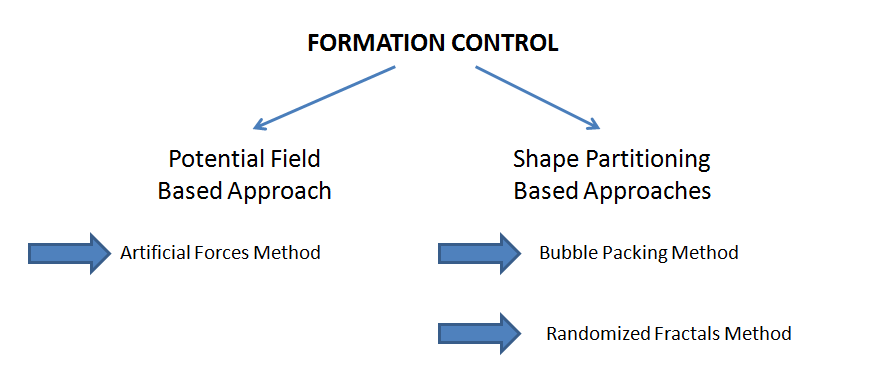
\includegraphics[scale = 0.60]{methods}
\end{figure}		
		
\subsection{Potential Field Based Approach}

\subsubsection{Artificial Forces Method} \label{Artificial Forces Ref} \label{Artificial_forces_ref}
In Artificial Forces method we have implemented potential fields over each agent arised from the interactions between agents, formation shape and environment. The positions of the agents at the formation shape  are determined with local equilibrium of the swarm in which every agent is at balance under the total force acting from the environment. There are basically three different kinds of artificial forces named; intermember forces representing the forces created by the other agents in the swarm to achieve collision avoidance, the attractive forces representing the forces created by the desired formation shape to attract the agent into the shape and repulsive forces created by the formation shape to keep agents inside the desired formation shape. It is possible to augment these type of forces for specific tasks and objectives. For example, obstacle forces created by the obstacles in the environment can be implemented to achieve obstacle avoidance. Since the method to calculate the artificial forces involves contour integrals, it will be useful to give mathematical definition of contour integrals.
		
Consider a curve $C$ which is a set of points $z = (x,y)$ in the complex plane defined by \cite{wiki_contour}

\begin{equation}
x = x(t),   \hspace{0.1cm} y = y(t),  \hspace{0.1cm} a\leq t \leq b
\end{equation}

where $x(t)$ and $y(t)$ are continuous functions of the real parameter $t$.  It is possible to write
		
\begin{equation}
z(t) = x(t)+iy(t),   \hspace{0.1cm} a\leq t \leq b
\end{equation}
		
This curve is called smooth if $z(t)$ has continuous derivative for all points along the curve, and it is called simple if it does not cross itself as defined in Equation \ref{crossitself}

\begin{equation} \label{crossitself}
z(t_1) \neq z(t_2)   \hspace{0.1cm} whenever   \hspace{0.3cm} t_1\neq t_2
\end{equation}
		
On the other hand if  $z(a)=z(b)$ is the only intersection point, the curve is said to be simple closed curve \cite{wiki_contour}. Regarding with these given definitions, an example for a  simple smooth closed curve is illustrated in Figure \ref{simple_closed_curve_ref}

\begin{figure}[H]
\caption{A Simple Closed Curve} \label{simple_closed_curve_ref}
\centering
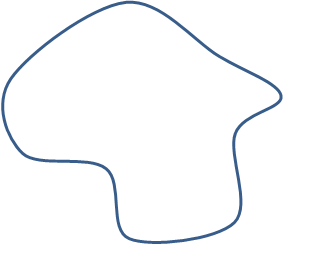
\includegraphics[scale = 0.60]{simple_closed_curve}
\end{figure}
		
Let $f(z)$ is a complex function in a domain $D$ in the complex plane and let $C$ be simple closed contour contained in $D$ with initial point $a$ and terminal point  $b$. It is possible to take the integral of $f(z)$ along the contour $C$ \cite{wiki_contour}
		
\begin{equation}
\oint_C f(z) dz = \int_{a}^{b} f(z(t))\frac{dz(t)}{dt} dt
\end{equation}
		
where
\begin{equation}
\frac{dz(t)}{dt} = \frac{dx(t)}{dt} + i\frac{dy(t)}{dt},   \hspace{0.1cm} a\leq t\leq b
\end{equation}
		
To simplify this equation, one can write $f(z) = u(x,y) + iv(x,y)$ and $dz = dx + idy$ into the statements,
		
\begin{align} \label{contour_integral}
\begin{split}
\oint_C f(z)dz & = \oint_C u dx - v dy + i \oint_C u dy + v dx \\
&= \int_{a}^{b}\left[u(x(t),y(t) )\frac{dx(t)}{dt} - v(x(t),y(t) )\frac{dy(t)}{dt}\right]dt\\
& \hspace{0.4cm} + i\int_{a}^{b} \left[u(x(t),y(t) )\frac{dy(t)}{dt} + v(x(t),y(t) )\frac{dx(t)}{dt}\right]dt
\end{split}
\end{align}

We have used this explicit form of the contour integrals in utility functions described in the following section. 		
		
\paragraph{Utility Functions}\hspace{0pt} \\
As it is mentioned in the Section \ref{Objectives}, the formation shapes will be simple closed contours which cannot be identified analytically. Definitions of the utility functions given in the following section are given with continuous contour integrals which requires the analytical expression of the curve on which the integral will be taken. In our thesis work, we have modified these expressions in discrete domain to provide a solution to  these type of calculations without analytical expressions of the closed curves.\\

\textit{ 		1- Cauchy Winding Number:} \\ 
Cauchy winding number of a curve in the plane around a given point is the number of times that curve travels counter-clockwise around the point. Suppose $C$ is the closed curve which is a set of points $z=(x,y)$ in the complex plane  and $z_i$ is a point to check whether it is inside of the curve or not, then the Cauchy winding number is \cite{17} :
					
\begin{equation}
 n(C,z_i) = \frac{1}{2\pi i}\oint_C \frac{dz}{z-z_i}
\end{equation}
		
The winding number for agent $i$ in the swarm,

\begin{equation}
n(C,z_i) = \left\{ \begin{array}{rl}
1 &\mbox{ when member i is inside C} \\
0 &\mbox{ when member i is outside C}
\end{array} \right.
\end{equation}

We have used this winding number to switch on/off some of the artificial forces while the agent is inside or outside of the formation shape. We have redefined this statement in discrete domain as:
\begin{equation}
n(C,z_i) = \frac{1}{2\pi i} \oint_C f(z)dz
\end{equation}

where 

\begin{equation}
f(z) = \frac{1}{z-z_i}
\end{equation}
		
Function of $f(z)$ can be partitioned into real and complex parts as:

\begin{equation}
u(x,y) = real(f(z))  \hspace{0.2cm} and \hspace{0.2cm} v(x,y) = imag(f(z))
\end{equation}
		
partitioning this function as mentioned in Equation \ref{contour_integral}
\begin{equation}
\oint_C f(z)dz  = \oint_C u dx - v dy + i \oint_C u dy + v dx 
\end{equation}

then

\begin{equation}
n(C,z_i)  = \frac{1}{2\pi i} \left[\int_{a}^{b} \left(u\frac{dx}{dt} - v\frac{dy}{dt}\right)dt + i\int_{a}^{b}\left(u\frac{dy}{dt} + v\frac{dx}{dt}\right)dt\right]
\end{equation}
		
Discrete contour integral representation of this equation is
		
\begin{equation}
n(C,z_i)  = \frac{1}{2\pi i} {\left[\sum_{k=1}^{K} {A_k} + i\sum_{k=1}^{K} {B_k}\right]}
\end{equation}

where
\begin{equation}
A_k = u(x_{k+1} - x_k ) - v(y_{k+1} -y_k )
\end{equation}

\begin{equation}
B_k = u(y_{k+1} - y_k ) + v(x_{k+1} - x_k)
\end{equation}


\begin{equation}
\norm{z_k - z_{k-1}} = \norm{z_{k+1} - z_k}, \hspace{0.2cm}  \forall k ;  \hspace{0.2cm} k=1,2,...,K \hspace{0.2cm} when  \hspace{0.2cm} K \to\infty
\end{equation}

The assumption of $K \to\infty$ makes it possible to calculate the integral of Cauchy winding number with a small error with large number of $K$ which can be achieved by partitioning the desired formation shape  into small pieces with equal $p2$ norms. We have used this approach to provide representations of the contour integrals in discrete domain. 

Figure \ref{iceride_disarida_refe} shows the test results for the grid map of an environment with a formation shape, where green dots represents the inner points of formation shape and red dots represents the outer points of the formation shape. Inner points in the grid map have a Cauchy winding number of 1, and the outer points have a Cauchy winding number of 0 .

\begin{figure}[H]
\centering
\captionsetup{format=hang,justification=centerfirst}
\caption{Formation Shape in an Environment} \label{iceride_disarida_refe}
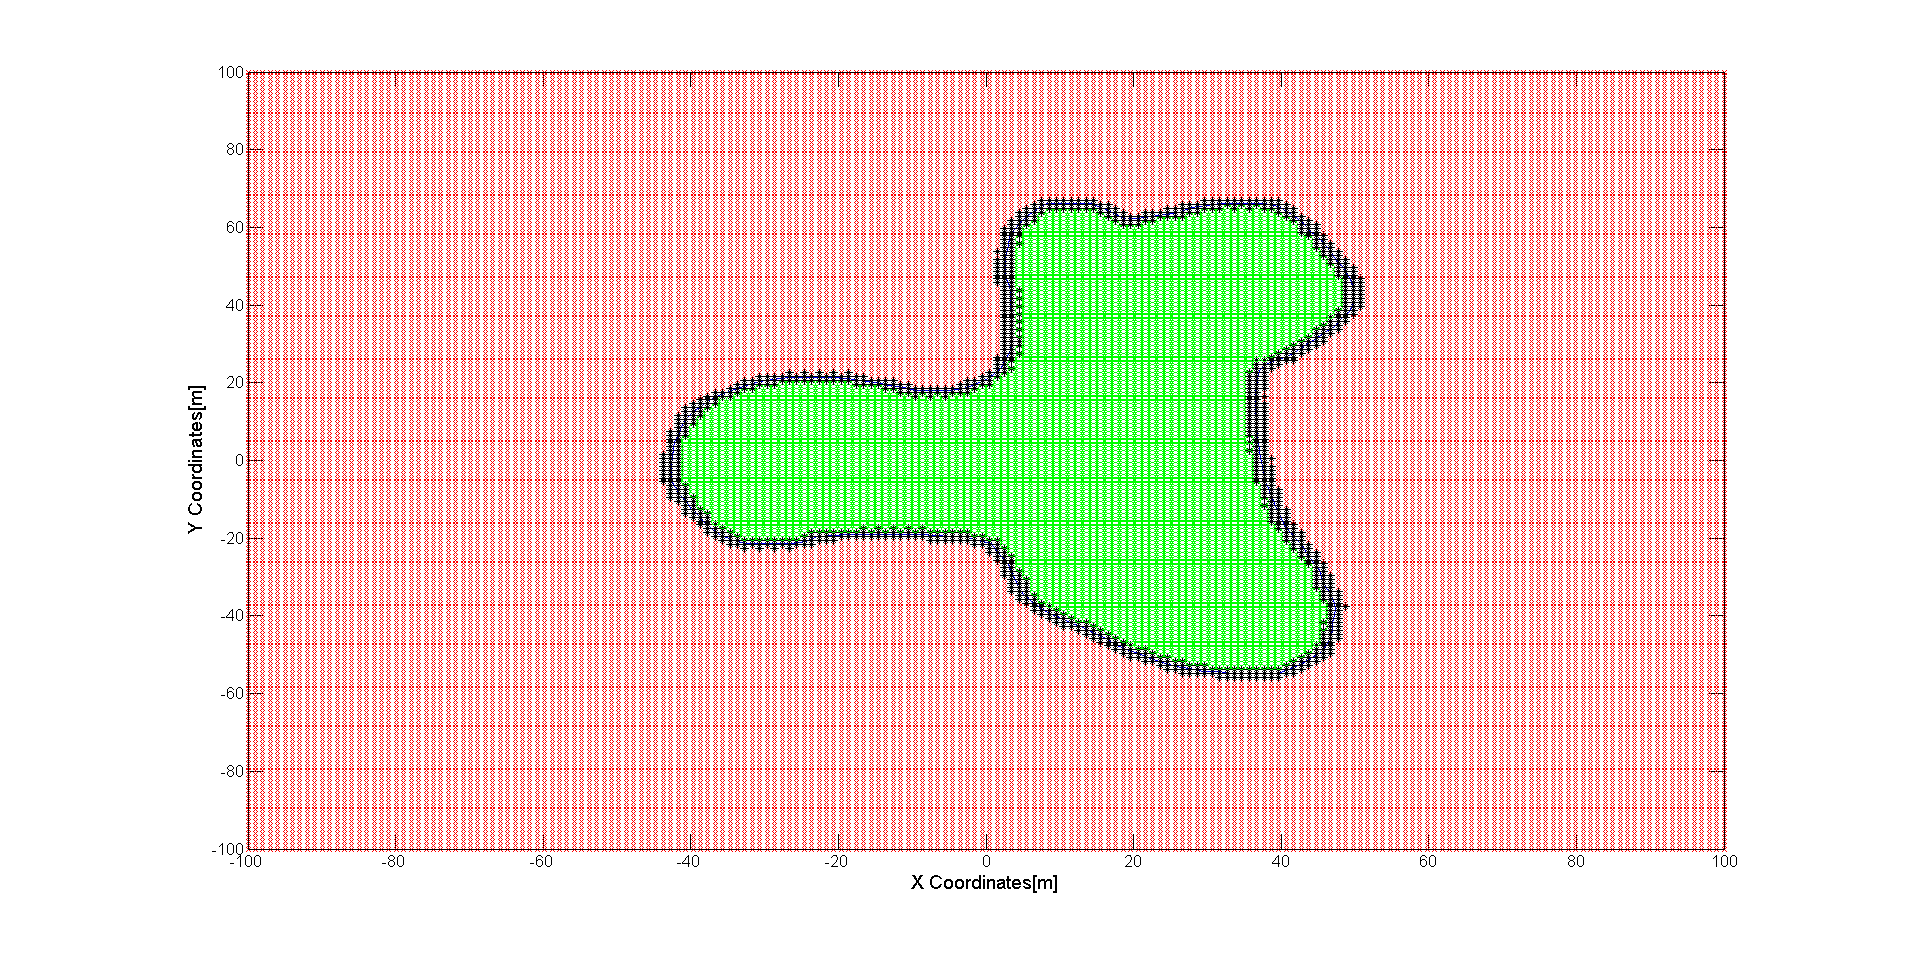
\includegraphics[scale = 0.28]{iceride_disarida}
\end{figure}

\textit{ 	2- Length of a formation shape} \\ 
The length of a formation shape can be calculated with the equation of \cite{17};
		
\begin{equation}
l(C)= \oint_C \norm{dz}
\end{equation}
		
We have redefined this expression for this contour integral with points of   $z_k = (x_k,y_k)$ in the complex plane

\begin{equation}
l(C) = \sum_{k=1}^{K}\sqrt{(x_{k+1} - x_k)^2 + (y_{k+1} - y_k)^2}
\end{equation}

where

\begin{equation}
\norm{z_k - z_{k-1}} = \norm{z_{k+1} - z_k}, \hspace{0.2cm}  \forall k ;  \hspace{0.2cm} k=1,2,...,K \hspace{0.2cm} when  \hspace{0.2cm} K \to\infty
\end{equation}
		
\textit{ 	3-Center of a Formation Shape} \\ 	
The center of a formation shape can be calculated with the equation of \cite{17};

\begin{equation} \label{center_formation_ref}
 z_c = \frac{\oint_C z\norm{dz}}{l(C)}
\end{equation}
		
We have redefined the discrete domain expression for Equation \ref{center_formation_ref} with points of  $z_k = (x_k,y_k)$ in the complex plane

\begin{align}
\begin{split}
&z_{cx} = \frac{\sum_{k=1}^{K}x(k)}{K}  \\
&z_{cy} = \frac{\sum_{k=1}^{K}y(k)}{K}  
\end{split}
\end{align}
		
where $z_{cx}$ and $z_{cy}$ are the $x$ and $y$ coordinates of the center of formation shape respectively and

\begin{equation}
\norm{z_k - z_{k-1}} = \norm{z_{k+1} - z_k}, \hspace{0.2cm}  \forall k ;  \hspace{0.2cm} k=1,2,...,K \hspace{0.2cm} when  \hspace{0.2cm} K \to\infty
\end{equation}

\textit{ 	4- Area of a Formation Shape} \\ 		
Green's theorem can be used to calculate the area of a closed curve. According to this theorem, the area of $D$ given by the double integral \cite{calculus}

\begin{equation}
 A = \int\int_D dA
\end{equation}
		
can be calculated with counter-clockwise order line integral of

\begin{equation}
 A = \oint_D F ds = \frac{1}{2} \oint_D xdy - ydx
\end{equation}

where

\begin{equation}
F(x,y) = (-y/2,x/2)
\end{equation}
		
This contour integral can be reduced down to

\begin{align} \label{area_formation_ref}
\begin{split}
Area &= \frac{1}{2} \oint_C xdy - \frac{1}{2} \oint_C ydx \\
&= \frac{1}{2} \int_{t=a}^{b} x(t)\frac{dy(t)}{dt}dt - \frac{1}{2} \int_{t=a}^{b}y(t)\frac{dx(t)}{dt}dt
\end{split}
\end{align}
		
We have implemented the expression in Equation \ref{area_formation_ref} in discrete domain with points of  $z_k = (x_k,y_k)$ in the complex plane
			
\begin{equation}
Area = \frac{1}{2} \sum_{k=1}^{K} x_k(y_{k+1} - y_k) - \frac{1}{2} \sum_{k=1}^{K}y_k(x_{k+1} - x_k)
\end{equation}
			
where

\begin{equation}
\norm{z_k - z_{k-1}} = \norm{z_{k+1} - z_k}, \hspace{0.2cm}  \forall k ;  \hspace{0.2cm} k=1,2,...,K \hspace{0.2cm} when  \hspace{0.2cm} K \to\infty
\end{equation}

\paragraph{Artificial Forces}\hspace{0pt} \\ 
Artificial forces are defined to gather the agents inside a formation shape and make them distributed homogeneously in the shape. It is possible to define some additional artificial forces to implement features like obstacle$\&$collision avoidance or smooth transitions between the boundaries of the formation shape. We have implemented attractive forces, repulsive forces, intermember forces, obstacle forces and transition forces to generate individual control laws for all agents in the swarm. Summation of these different types of artificial force components define the individual control law of a single agent. Suppose the state of a member $i$ is described by

\begin{equation}
X_i = \begin{bmatrix}
z_i\\ \dot{z}_i
\end{bmatrix}
\end{equation}

where  $z_i \in C$, represents the position of the $i^{th}$ member of the swarm. The state of the whole swarm $x= \begin{bmatrix}
X_1 & X_2 & ... X_n
\end{bmatrix}$ is determined by the linear equations of \cite{17}

\begin{equation}
\dot{x} = Ax + Bu
\end{equation}

where

\begin{align}
\begin{split}
&A = diag\left(\hat{A}\right)_{nxn}\\
&B = \frac{1}{m} diag\left(\hat{B}\right)_{nxn}
\end{split}
\end{align}

with

\begin{equation}
\hat{A} = \begin{bmatrix}
0&1\\0&0
\end{bmatrix} , \hspace{0.2cm} \hat{B} = \begin{bmatrix}
0&1
\end{bmatrix}
\end{equation}
			
The vector for individual control laws of the swarm

\begin{equation}
u = \begin{bmatrix}
u_1 & u_2 & ... & u_n
\end{bmatrix}
\end{equation}

where

\begin{equation}
u_i = F_{i,a} + F_{i,r} + F_{i,m} + F_{i,t}
\end{equation}

We have defined the concept of "coverage circle"	for the agents which will be used in the artificial forces calculations. Coverage circle of agent $i$, $C_i$, is defined as the circle with minimum radius which can cover the whole agent's collision surface. The radius of this circle is given with $d_c$. Some of the examples of coverage circles for different types of mobile robots are illustrated in Figure \ref{coverage_circle_ref} below
		
\begin{figure}[H]
\caption{Coverage Circles of Different Types of Agents} \label{coverage_circle_ref}
\centering
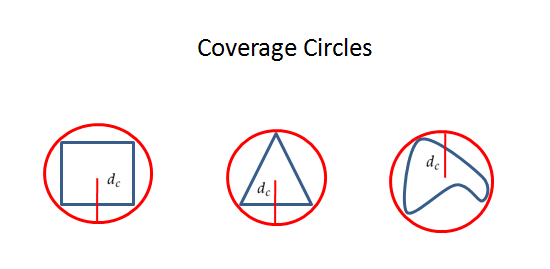
\includegraphics[scale = 0.60]{coverage_circles}
\end{figure}
		
Different artificial force components are described in details at the following section. \newline

\textit{			1- Attractive Forces} \\ 
Attractive forces are the artificial force components generated by the formation shape to attract the agent towards the center of the formation .They are active when the agents are outside of the shape. 

\begin{figure}[H]
\caption{Attractive Forces Generated by the Formation Shape}
\centering
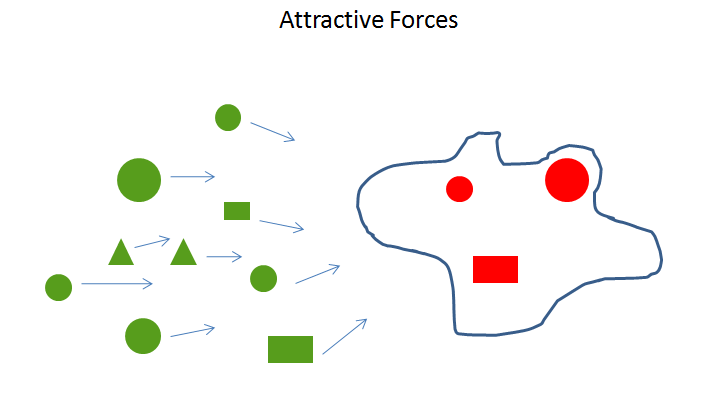
\includegraphics[scale = 0.60]{attractive_forces}
\end{figure}	

The equations for the attractive forces are defined as follows in \cite{17}:			

\begin{equation} \label{samitha_attractive}
F_{i,a} := k_a (1-n(C,\alpha X_i)) \oint_C(z-\alpha X_i)\norm{dz}
\end{equation}

where $k_a$ is the variable gain and $\alpha = \begin{bmatrix}
1 & 0
		\end{bmatrix}$. Equation \ref{samitha_attractive} takes the contour integral of the curve defined by desired formation shape. Since we don't have the analytical expression of the desired formation shape, we have redefined this expression in discrete domain. The representation of the attractive forces on agent $i$ on $z_i = (x_i, y_i)$ with the points of  $z_k = (x_k,y_k)$ of formation shape in the complex plane \cite{17}:

\begin{align}
\begin{split}
& F_{iax} =\frac{k_a (1-n(C,\alpha X_i))}{l(C)}  \sum_{k=1}^{K} (x_k  - x_i)\\
& F_{iay} =\frac{k_a (1-n(C,\alpha X_i))}{l(C)}  \sum_{k=1}^{K} (y_k  - y_i)\\
\end{split}
\end{align}
			
where

\begin{equation}
\norm{z_k - z_{k-1}} = \norm{z_{k+1} - z_k}, \hspace{0.2cm}  \forall k ;  \hspace{0.2cm} k=1,2,...,K \hspace{0.2cm} when  \hspace{0.2cm} K \to\infty
\end{equation}
			
and $F_{iax} , F_{iay} $ are the attractive force components in $x,y$ coordinates respectively. We have divided the artificial forces by $l(C)$ to prevent the dependency of the force on the different length of curves.
			
\textit{	2- Repulsive Forces} \\ 
Repulsive forces are the artificial force components generated by the formation shape to keep the agents inside the shape. They are active when the agents are inside the shape. 
					
\begin{figure}[H]
\caption{Repulsive Forces Generated by the Formation Shape}
\centering
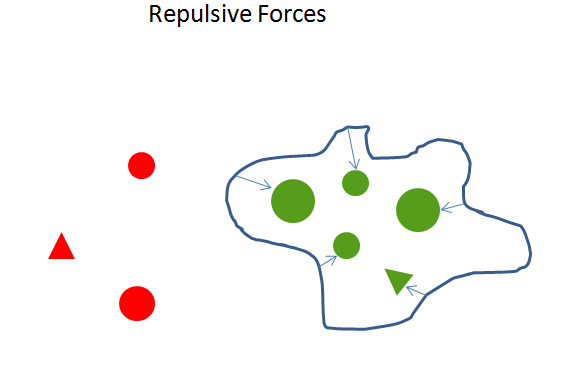
\includegraphics[scale = 0.60]{repulsive_forces}
\end{figure}
							
The equations for the repulsive forces are defined as follows \cite{17}:	

\begin{equation} \label{samitha_repulsive}
F_{i,r} := k_r  n(C,\alpha X_i) \oint_C \left[\frac{\alpha X_i - z}{\norm{\alpha X_i - z}^3}\right] \norm{dz}
\end{equation}

where $k_r$ is the variable gain for the repulsive forces. We have redefined the Equation \ref{samitha_repulsive} in discrete domain to calculate the repulsive forces for complex shapes. The representation of the repulsive forces on agent $i$ on $z_i = (x_i, y_i)$ with the points of  $z_k = (x_k,y_k)$ of formation shape in the complex plane:

\begin{align}
\begin{split}
& F_{irx} = k_r n(C,\alpha X_i)  \sum_{k=1}^{K} \frac{x_i - x_k}{\norm{\alpha X_i - z_k}^3}\\
& F_{iry} = k_r n(C,\alpha X_i)  \sum_{k=1}^{K} \frac{y_i - y_k}{\norm{\alpha X_i - z_k}^3}
\end{split}
\end{align}
				
where

\begin{equation}
\norm{z_k - z_{k-1}} = \norm{z_{k+1} - z_k}, \hspace{0.2cm}  \forall k ;  \hspace{0.2cm} k=1,2,...,K \hspace{0.2cm} when  \hspace{0.2cm} K \to\infty
\end{equation}
						
and $F_{irx} , F_{iry} $ are the repulsive force components in $x,y$ coordinates respectively. \newline
						
\textit{		3- Inter-member repulsion forces} \\ 
Intermember forces are the artificial force components generated by the agents in the swarm to avoid collisions between themselves. 
			
\begin{figure}[H]
\caption{Intermember Forces Generated by Agents}
\centering
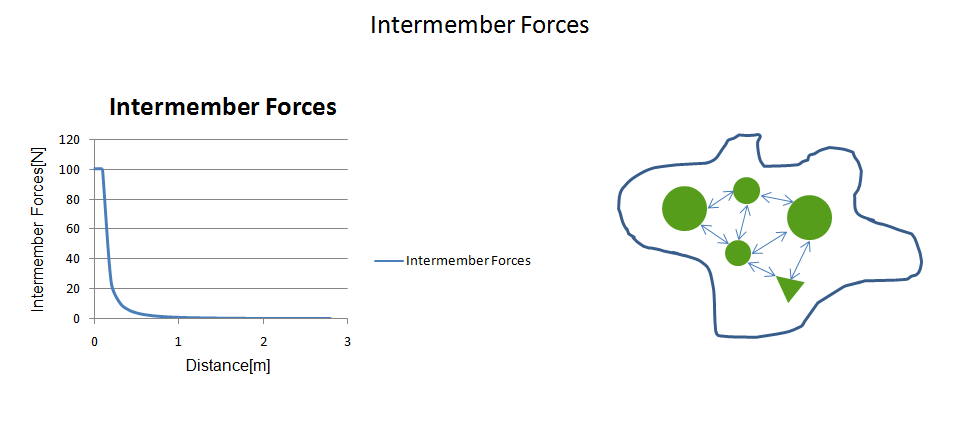
\includegraphics[scale = 0.60]{intermember_forces}
\end{figure}
			
The equations for the intermember forces on the agent $i$ on $z_i = (x_i, y_i)$  in the complex plane \cite{17},
			
\begin{equation}
F_{i,m} = k_m \sum_{j=1, j\neq i}^{N}\frac{\alpha X_i - \alpha X_j}{(\norm{\alpha X_i - \alpha X_j})} \frac{1}{(\norm{\alpha X_i - \alpha X_j} - d_o)^2}
\end{equation}
			
where $d_o$ is the total distance between the center of coverage circles of agents which can be calculated with

\begin{equation}
 d_o = d_{c_i} + d_{c_j}
\end{equation}			

The force components in x,y coordinates respectively,

\begin{align}
\begin{split}
&F_{imx} = k_m \sum_{j=1, j\neq i}^{N}\frac{x_i- x_j}{\norm{\alpha X_i - \alpha X_j}}  \frac{1}{(\norm{\alpha X_i - \alpha X_j} - d_o)^2}\\
&F_{imy} = k_m \sum_{j=1, j\neq i}^{N}\frac{y_i- y_j}{\norm{\alpha X_i - \alpha X_j}}  \frac{1}{(\norm{\alpha X_i - \alpha X_j} - d_o)^2}\\
\end{split}
\end{align}
		
where $k_m$ is the variable gain for the intermember forces.  \newline
			
\textit{4- Transition Forces} \\ 		
Transition forces are the artificial force components to force the agent to get inside the formation shape when they are close to the boundaries. Since the attractive forces have a decreasing nature while the agent getting closer to the formation shape, we need to add this type of forcing function to ensure the agents to get inside the shape. Transition forces are active outside of the desired formation shape.
			
\begin{figure}[H]
\caption{Comparison of Attractive and Transition Forces}
\centering
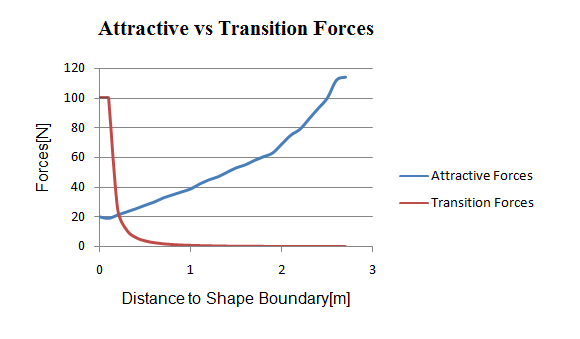
\includegraphics[scale = 0.80]{transition_forces}
\end{figure}		

The equation for the transition forces are defined as follows \cite{17}:	
				
\begin{equation}
F_{i,t} = k_t (1-n(C,\alpha X_i) \oint_C \frac{z-\alpha X_i}{\norm{z-\alpha X_i}}\norm{dz}
\end{equation}
				
where $k_t$ is the variable gain for the transition forces. The representation of the transition forces on agent $i$ on $z_i = (x_i, y_i)$ with the points of  $z_k = (x_k,y_k)$ of formation shape in the complex plane:
			
\begin{align}
\begin{split}
&F_{itx} = k_t  (1-n(C,\alpha X_i) \sum_{k=1,}^{K}\frac{x_k- x_i}{\norm{\alpha X_i - z_k}}\\
&F_{ity} = k_t  (1-n(C,\alpha X_i) \sum_{k=1,}^{K}\frac{y_k- y_i}{\norm{\alpha X_i - z_k}}\\
\end{split}
\end{align}
			
where  $F_{itx} , F_{ity} $ are the transition force components in $x,y$ coordinates respectively and

\begin{equation}
\norm{z_k - z_{k-1}} = \norm{z_{k+1} - z_k}, \hspace{0.2cm}  \forall k ;  \hspace{0.2cm} k=1,2,...,K \hspace{0.2cm} when  \hspace{0.2cm} K \to\infty
\end{equation}					
			
\textit{			5- Obstacle forces} \\ 
Obstacle forces are the artificial force components generated by the obstacles in the environment to achieve obstacle avoidance of the agents during formation control. 	
The equation for the obstacle forces are defined as follows \cite{17}:	
			
\begin{equation} \label{samitha_obstacle}
F_{i,o} := k_o  \oint_O \left[\frac{\alpha X_i - z_o}{(\norm{\alpha X_i - z_o} - d_{c_i})^4}\right] \norm{dz_o}
\end{equation}
			
where $k_o$ is the variable gain for the transition forces and $d_{c_i}$ is the radius of coverage circle of agent $i$ . This contour integral is taken on the curve of the obstacle with  points of $z_o = (x_o,y_o)$ in the complex plane. Obstacles in the workspace are assumed to have complex shapes without mathematical definitions. Because of this, we have expressed the Equation \ref{samitha_obstacle} in discrete domain. The representation of the obstacle forces on agent $i$ on $z_i = (x_i, y_i)$ with the points of  $z_{ok} = (x_{ok},y_{ok})$ of formation shape in the complex plane:
			
\begin{align}
\begin{split}
& F_{iox} = k_o   \sum_{k=1}^{K} \frac{x_i -x_{ok}}{(\norm{\alpha X_i - z_{ok}} -d_{c_i})^4}\\
& F_{ioy} = k_o   \sum_{k=1}^{K} \frac{y_i - y_{ok}}{(\norm{\alpha X_i - z_{ok}} -d_{c_i})^4}\\
\end{split}
\end{align}
			
where

\begin{equation}
\norm{z_k - z_{k-1}} = \norm{z_{k+1} - z_k}, \hspace{0.2cm}  \forall k ;  \hspace{0.2cm} k=1,2,...,K \hspace{0.2cm} when  \hspace{0.2cm} K \to\infty					
\end{equation}
			
\paragraph{Buffer Zone Implementation}\hspace{0pt} \\
The attractive and transition forces are defined to be active when the agents are outside of the shape. On the other hand, the repulsive forces are active when agents are inside the shape. Because of the sharp transitions on the total artificial force acting on an agent which is crossing the boundary of the formation shape, it is possible to have a chattering effect. To avoid this chattering effect and provide a smooth transition of the agent to pass the boundary of formation shape, we have implemented a buffer zone defined around the boundaries of the formation shape. The main approach during the transition on the boundaries is to dynamically change the variable gains of these artificial forces linearly between zero and nominal values at the boundary conditions. The variable gains of the attractive and transition force components have their nominal values at the outer boundary of shape and these gains are decreased down to zero linearly while travelling towards the inner boundary of the shape. On the other hand, the variable gain for the repulsive forces has its nominal value at the inner boundary of the shape and this gain is decreased down to zero linearly while travelling towards to outer boundary of the shape.
     
\begin{figure}[H]
\caption{Transition of the Artificial Forces on Buffer Zone}
\centering
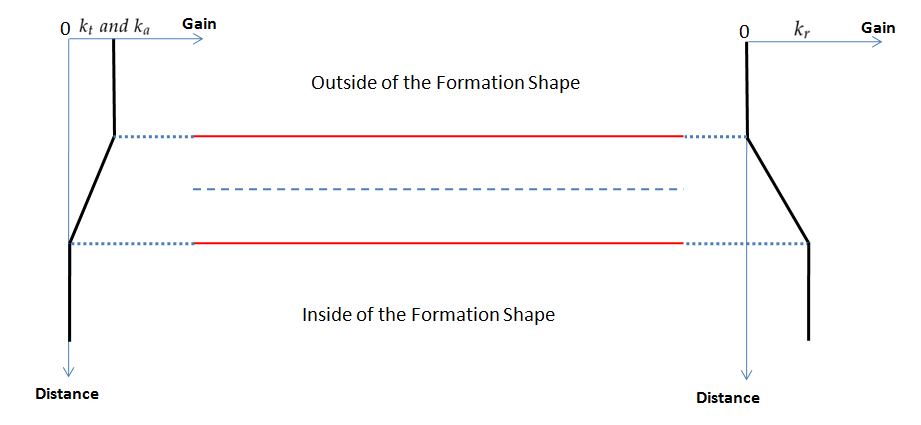
\includegraphics[scale = 0.50]{buffer_zone}
\end{figure}
					
\subsection{Shape Partitioning Methods} \label{shapepartition_ref}
In shape partitioning methods we have reduced down the formation control problem into two subproblems. The first part of the solution is to partition the desired formation shape into potential goal states according to the agent types to cover the desired formation shape homogeneously. We have proposed two different solutions to the shape partitioning problem in this thesis work, Bubble Packing method and Randomized Fractals method. The second part of the solution is the decision process to assign the agents to these goal states continuously to minimize the total displacement of swarm while achieving the desired formation shape. During this decision process, the cost of reaching different goal states is defined with the displacement on the shortest path while reaching that goal state. Our algorithm tries to reduce down the total cost value by assigning each agent to proper goal states.

Shape partitioning methods have an approach to direct the agents to the goal states in which they have assigned dynamically. In this approach it is still needed to have collision avoidance algorithms to prevent the agents to collide with each other and workspace obstacles while travelling towards these goal states. For this purpose we add obstacle and inter-member forces to the individual control laws defined in shape partitioning approaches.
			
\subsubsection{Determining the Potential Goal States} \label{Partitioning_ref}
\paragraph{Bubble Packing Method} \hspace{0pt} \\				
Bubble Packing method is widely used in mesh generation problems. It basically depends on covering a curve, surface or a volume with a proper number of bubbles by packing them tightly which mimic a Voronoi diagram, from which a set of well-shaped Delaunay triangles can be created by connecting the centers of the bubbles \cite{27}.  The algorithm places the bubbles with their initial conditions in the environment and apply them interbubble forces which imitates the Van der Waals forces between the molecular bonds  to distribute the bubbles homogeneously inside the shape. Here, the main idea is to generate a mesh for a surface with identical bubbles to mimic a regular Voronoi diagram with the vertices represented by the centers of these bubbles. On the other hand, adaptive population control  methods are developed to increase the number of bubbles to fill the gaps in the shape and to remove the excess bubbles which are overlapping with each other and the shape boundaries \cite{27}. 

Since the numbers and the the radius of coverage circles defined at Section \ref{Artificial Forces Ref} are predetermined in our formation control problem, the general bubble meshing algorithm have to be adapted to meet the requirements for shape partitioning in formation control.  In our project we have adapted this algorithm to represent the agents in the swarm as bubbles with the radius of their coverage circles and create a mesh by using these bubbles. The details of the implementation are given in following sections.\newline
			
\textit{			I - Initial Placements of the Bubbles} \\ 
The initial bubble placements are important because it will greatly reduce the convergence time of the partitioning process. In this work, we have initiated the bubbles close to the center of the formation shape randomly. The algorithm for initial bubble placements is implemented as follows:
			
\begin{algorithm}[H]
\KwData{Set of Bubbles, Desired Formation Shape }
\KwResult{Initial Placements of the Bubbles }
Initialize free configuration space $C_{free}$ as the desired formation shape \newline
\For{<Each Bubble $i$>}
{		
*Calculate the free configuration space,$C_{free}$, for bubble $i$\;
*Put the Bubble $i$ to the closest point to  formation center  $z_c$  in the free configuration space\;
*Add the agent $i$ into the configuration space as an obstacle \;
}\		
\caption{INITIALIZE$\_$BUBBLE$\_$POSITIONS} \label{intial_buble}
\end{algorithm}
		
The term free configuration space $C_{free}$ will be analyzed in detail in Section \ref{DecisionProcess Ref}. A simulation output, with a sample formation shape and 11 coverage circles which are representing a heterogeneous swarm composed of agents from 3 different size is illustrated in Figure \ref{algorithm1_ref} below.
		
\begin{figure}[H]
\caption{Initialization of the Bubble Packing Algorithm} \label{algorithm1_ref}
\centering
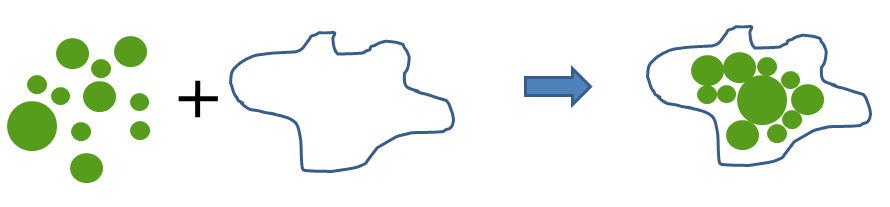
\includegraphics[scale = 0.50]{bubble_packing}
\end{figure}
				
\textit{			II- Bubble Meshing Process } \\ 
The bubbles are distributed homogeneously with this process under two kinds of forces, interbubble forces and shape repulsive forces. The interbubble forces are proximity-based forces so that a system of bubbles is in equilibrium when bubbles are distributed over the whole formation shape. The implemented force equation is given
		
\begin{equation}
f_i(l) = \left\{ \begin{array}{rl}
al^3 + bl^2 + cl + d &\mbox{ when 0 $\leq$ l $\leq$ $l_0$} \\
0                               &\mbox{ l > $l_0$}
\end{array} \right.
\end{equation}

where $l$ is the distance between the centers of the related bubbles and $a,b,c,d$ and $l_0$ are the variables to tune the force acting on the bubbles. 

\begin{figure}[H]
\caption{Interbubble Forces}
\centering
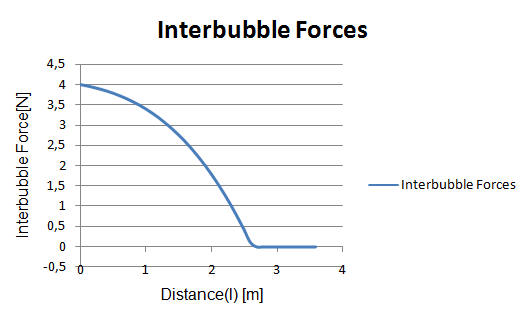
\includegraphics[scale = 0.70]{interbubble_forces}
\end{figure}
	
The shape repulsive forces have the same characteristics with the repulsive artificial forces discussed in Section \ref{Artificial Forces Ref}. The representation of shape repulsive forces for the desired formation shape $C$ with the points of  $z_k = (x_k,y_k)$ the complex plane:
	
\begin{equation} \label{buble_repulsive}
f_r(X_i) := \oint_C \left[\frac{\alpha X_i - z}{\norm{\alpha X_i - z}^3}\right] \norm{dz}
\end{equation}

where $k_r$ is the variable gain for the shape repulsive forces. We have defined the shape repulsive forces on agent $i$ in discrete domain with the points of  $z_k = (x_k,y_k)$ on formation shape in the complex plane:

\begin{equation}
f_r(X_i) = \sum_{k=1}^{K} \frac{\alpha X_i - Z_k}{\norm{\alpha X_i - z_k}^3}
\end{equation}
				
where

\begin{equation}
\norm{z_k - z_{k-1}} = \norm{z_{k+1} - z_k}, \hspace{0.2cm}  \forall k ;  \hspace{0.2cm} k=1,2,...,K \hspace{0.2cm} when  \hspace{0.2cm} K \to\infty					
\end{equation}
						

	
The bubbles are distributed homogeneously under the influence of these two forces and they get an equilibrium state in which the total net forces acting on individual bubbles reaches zero. Figure \ref{buble_ornek} shows a simulation output of Bubble Packing algoithm which is initialized with coverage circles derived from the output of the INITIALIZE$\_$BUBBLE$\_$POSITIONS algorithm. The coverage circles are homogeneously distributed in the formation shape with the help of inter-bubble and shape repulsive forces. The final equilibrium states of the bubbles determine the potential goal states $g_i \in G$  of the agents in the swarm to cover the formation shape.

\begin{figure}[H]
\caption{Bubble Packing Algorithm} \label{buble_ornek}
\centering
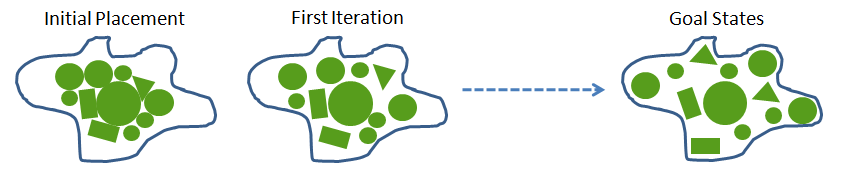
\includegraphics[scale = 0.62]{bubble_packing2}
\end{figure}

\paragraph{Randomized Fractals Method}\hspace{0pt} \\
Randomized fractals methods are used to cover surfaces or volumes randomly with fractals. The main idea is to fill the shapes iteratively with fractals which has the areas determined by the rule of \cite{26} :

\begin{equation} \label{fractals}
A_i = \frac{A}{\zeta(c,N)(i+N)^c}
\end{equation}

where $A$ is the total area to cover and $A_i$ is the area of the $i^{th}$ fractal. The parameters of $c$ and $N$ can be chosen to implement different changes on the fractals' areas with the increasing number of iterations with $c>1$ and $N>0$. Here  $\zeta$ is the Hurwitz function defined by

\begin{equation}
\zeta(c,N) = \sum_{i=0}^{\infty} \frac{1}{(i+N)^c}
\end{equation}

It is possible to write, 
	
\begin{equation}
\sum_{i=0}^{\infty}A_i = \sum_{i = 0}^{\infty}\left(\frac{A}{\zeta(c,N)(i+N)^c}\right)
\end{equation}
	
which tells us the sum of the all areas $A_i$ is the total area of $A$ and the algorithm is space filling. This approach implements the fractals infinitely by reducing the areas in accordance with the Equation \ref{fractals}, to cover the desired formation shape randomly. 

\begin{figure}[H]
\caption{Randomized Fractals \cite{26}}
\centering
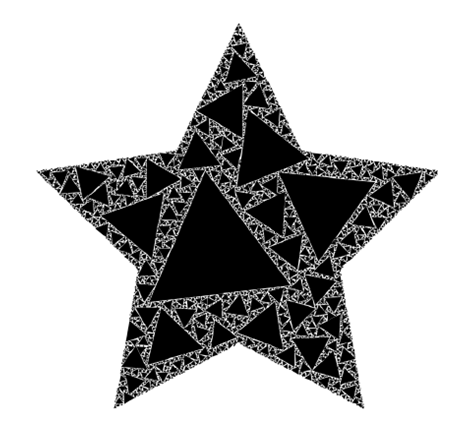
\includegraphics[scale = 0.60]{randomized}
\end{figure}
	
Types and the number of the agents, which will be represented with their coverage circles, are predetermined in our work. By using this constraint, we have adapted the randomized fractals algorithm as follows:
		
\begin{algorithm}[H]
\KwData{Set of Coverage Circles, Desired Formation Shape }
\KwResult{Potential Goal States }
Initialize free configuration space $C_{free}$ as the desired formation shape \newline
\For{<Each Coverage Circle $i$>}
{		
*Calculate the free configuration space $C_{free}$ for circle $i$\;
\eIf{$C_{free}  \neq Full$}{
*Put the circle $i$ randomly in $C_{free}$ \;
*Add the agent $i$ into configuration space as an obstacle \;
}{
*Break and warn the operator to increase the size of formation shape
}
}\												
\caption{RANDOMIZED$\_$FRACTALS$\_$ALGORITHM} 
\end{algorithm}
		
The algorithm iteratively checks the free configuration space that if there is enough space. If so, it inserts a coverage circle which is representing the current agent in the swarm, randomly in the desired formation shape. At the end of each insertion, it updates the free configuration space and jumps to next iteration. When algorithm terminates, the positions of the coverage circles which are randomly placed in desired formation shape gives us the goal states $g_i \in G$  of the agents. 

\begin{figure}[H]
\caption{Simulation Output of the Algorithm} \label{randomized_ornek}
\centering
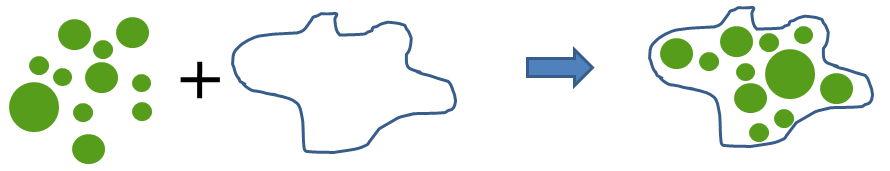
\includegraphics[scale = 0.60]{randomized_ornek}
\end{figure}

Figure \ref{randomized_ornek} shows a simulation output of the Randomized Fractals algorithm. In this figure, coverage circles are representing the members of a swarm which consist of 11 heterogeneous agents from 3 different sizes. These coverage circles are randomly distributed in the desired formation shape with the help of Randomized Fractals algorithm. Positions of the coverage circles define the goal states $g_i \in G$  of the agents in the formation shape. 

	
\subsubsection{Decision Process on Goal States}\hspace{0pt} \label{DecisionProcess Ref} \\
In Section \ref{Partitioning_ref}, we have reduced down the formation control problem in which every agent is expected to decide where to position in a given set of possible goal states $g_i \in G$ .  During this decision process, the cost of reaching different goal states will be the main criteria for each agent. Given goal states and cost values to these goal states, each agent must decide where to position in the formation. This process must be held to optimize the utility of swarm with a collaboration. It is obvious that some of the agents may want to choose the same goal point to reach, so the swarm must reach a global consensus on target points and cases including conflictions must be handled. Our main approach to provide a solution for this problem is to make each agent to calculate the costs of its own to reach the goal states $g_i \in G$ and then reach a global consensus with the other agents to minimize the overall displacements of the swarm. 

The algorithm which handles the assignment process of the agents to the goal states, is implemented in four stages. At the first stage, each agent calculates its own free configuration space. Secondly, agents calculate their visibility graphs by using their free configuration space. At the third stage,  agents calculate and report their costs to reach each of the goal states $g_i \in G$ with the help of Dijkstra's algorithm. These cost values are defined as the displacements to reach a goal state on shortest path.  Finally, agents are assigned to the goal states with the help of Hungarian algorithm which uses the cost values reported by the agents. Hungarian algorithm handles the assignment process to minimize the overall cost(i.e. total displacement) of the swarm.
	
\paragraph{Free Configuration Space}\hspace{0pt} \\
We have defined the shortest paths to the goal states of $g_i \in G$ in the free configuration space to avoid collisions with the workspace obstacles \cite{92}. In our implementation, each agent calculates its free configuration space by extracting their forbidden spaces from the configuration space itself. Forbidden space is calculated by augmenting the workspace obstacles with the help of Minkowski sums and we have implemented this process as follows.

Assume an environment with set of obstacles $S = \begin{Bmatrix}
P_1, P_2, .. P_t \end{Bmatrix}$. Configuration for agent $i$ can be described with the position of the center of its coverage circle with $R=\begin{Bmatrix}x_i, y_i\end{Bmatrix}$. Configuration space of $i^{th}$ agent is the workspace itself and represented by $C(R_i)$. This configuration space is composed of two subspaces; free configuration space and forbidden configuration space of agent $i$ \cite{92}.

\begin{equation}
C(R_i) = C_{free}(R_i,S) + C_{forb}(R_i,S)
\end{equation}

In our implementation each agent calculates its forbidden space by augmenting the workspace obstacles with the help of Minkowski sum method. Minkowski sum method is implemented as follows:

Let a single obstacle is described with a point set of $S_1$ and the agent is described with a point set of $S_2$. The Minkowski sum of these two sets $S_1 \subset R^2$ and $S_2 \subset R^2$ can be calculated with the following \cite{92},
	
\begin{equation}
S_1 \oplus S_2 := \begin{Bmatrix}
p+q : p \subset S_1, q \subset S_2
\end{Bmatrix} 
\end{equation}

where $p+q$ denotes the vector sum of the vectors $p$ and $q$.
		
\begin{figure}[H]
\caption{Forbidden Space Caused by an Obstacle \cite{92}} \label{yasakli_bolge}
\centering
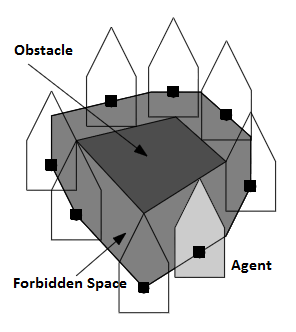
\includegraphics[scale = 0.75]{Forbidden}
\end{figure}
	
Figure \ref{yasakli_bolge} shows a forbidden space related with an obstacle. Forbidden space for agent $i$, $C_{forb}(R_i, S)$, is the sum of the forbidden spaces calculated for each obstacle in the environment \cite{92}. Agents extract their forbidden space $C_{forb}(R_i, S)$ from the configuration space itself to calculate their free configuration spaces.
	
\paragraph{Visibility Graphs and Dijkstra$'$s Algorithm}\hspace{0pt} \\
We have provided collision avoidance while travelling towards to the goal states $g_i \in G$ by defining the shortest paths in the free configuration spaces of the agents. In \cite{92}, an additional constraint for the shortest path is defined as follows : 

\begin{displayquote}
The shortest path between $p_{start}$ and $p_{goal}$ among a set $S$ of augmented polygonal obstacles consists of the arcs of the visibility graph $\gamma_{vis}(S^*)$ where $S^* := S \cup \begin{Bmatrix}
p_{start}, p_{goal}
\end{Bmatrix}$
\end{displayquote}

A visibility graph, $\gamma_{vis}(S^*)$, is a graph which is set of interior nodes representing the vertices of the set of obstacles, $S$, in the environment and edges which represents visible (which are not intersecting interior region of an obstacle) connections between these nodes \cite{92}.

In this project we have updated this constraint in our algorithm. We have inserted all of the goal states $g_i \in G$ in the visibility graphs of each agent to calculate the shortest paths to all of these goal states rather than a specific $p_{start}$ and $p_{goal}$ points given in the definition. In the implementation phase, we have used the obstacles which are augmented with the Minkowski sums to calculate the free configuration space. Let these set of augmented polygonal obstacles represented with $S_i \subset S$. 



Algorithm to calculate the visibility graph of  $S^* := S \cup \begin{Bmatrix}
g_i \in G
\end{Bmatrix}$
	
\begin{algorithm}[H]
\KwData{Set of Vertices Included in $S^*$ }
\KwResult{Visibility Graph of $S^*$ }
Initialize a graph $\gamma = (V,E)$ where $V$ is the set of all vertices in $S^*$ and $E = \oslash$  \\
\For{<all vertices $v \subset V$>}
{		
W = VISIBLE$\_$VERTICES($v$,S)\;
Add edges W to list E\;
}\

\caption{VISIBILITY$\_$GRAPH}
\end{algorithm}

where $VISIBLE$\_$VERTICES(v,S)$ algorithm checks whether line segments drawn from $v$ to all vertices in $S$ is intersecting an interior area of any obstacle in the environment and returns the non-intersecting edges.  By using this $VISIBILITY$\_$GRAPH$ algorithm, $SHORTEST$\_$PATH$ algorithm is defined as follows. \newline
	
\begin{algorithm}[H]
\KwData{A set $S$ of disjoint polygonal obstacles, position of agent, $p_{start}$, and all goal states $g_i \in G$}
\KwResult{The shortest collision-free paths from $p_{start}$ to all goal states $g_i \in G$}
* Assign $\gamma$ = VISIBILITY$\_$GRAPH$(S^*)$ \newline
* Assign each arc $(v,w)$ in $\gamma_{vis}$ a weight, which is the Euclidian length of line segment drawn from $v$ to $w$ \newline
\For{<Each goal state $g_i \in G$>}
{
* Use Dijkstra's algorithm to compute a shortest path between $p_{start}$ and $g_i \in G$ in $\gamma_{vis}$
}
\caption{SHORTEST$\_$PATH}
\end{algorithm}
  
\vspace{2cm}

\begin{figure}[H]
\caption{Shorthest Paths to Goal States $g_i \in G$ in a Visibility Graph} \label{dijksttae_visibility}
\centering
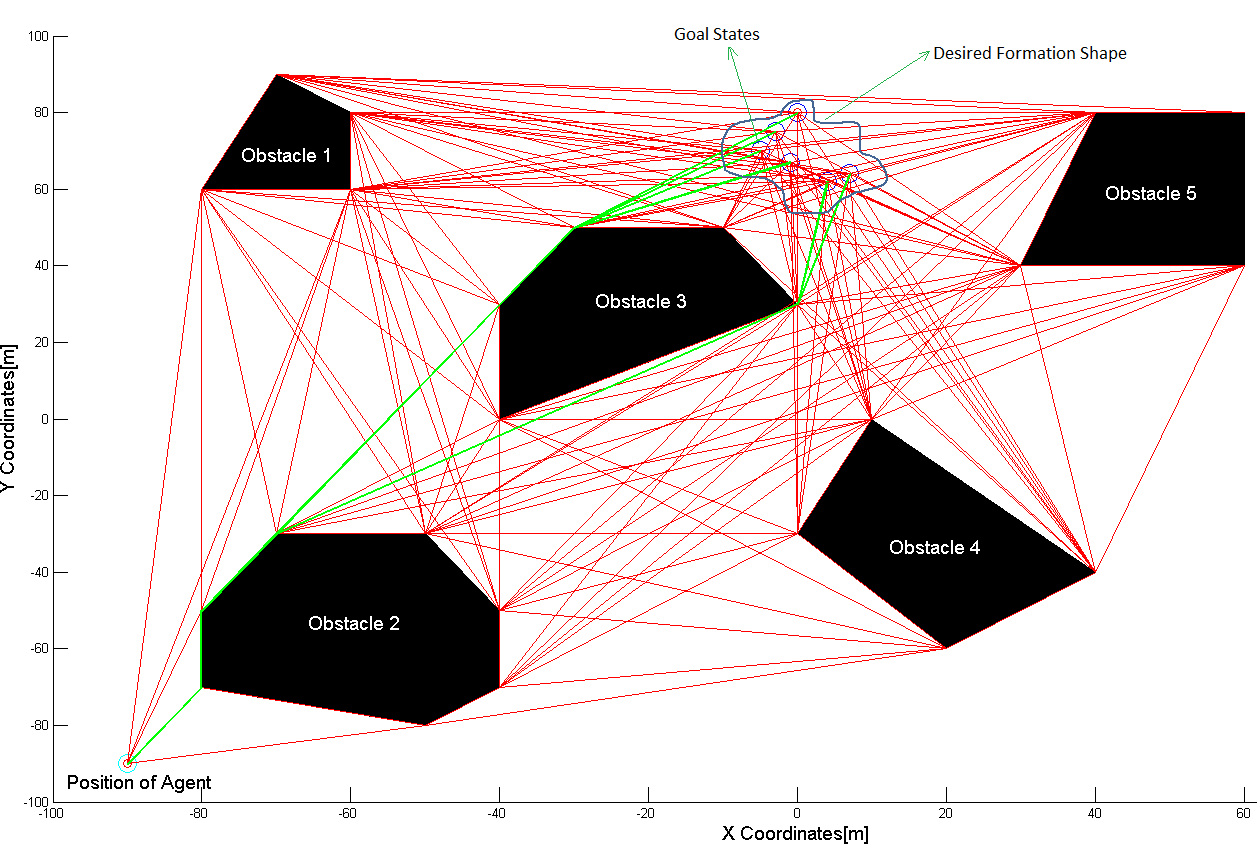
\includegraphics[scale = 0.40]{visgraph2}
\end{figure} 

Figure \ref{dijksttae_visibility} shows a simulation output executed with 5 workspace obstacles and 6 goal states in desired formation shape. In this algorithm, agent first calculates its own visibility graph by adding goal states $g_i \in G$ in graph as nodes. The visibility graph is illustrated with red edges in the figure. Then it calculates the shorthest paths to the goal states, which are given with green edges in the figure. We have used Dijkstra algorithm to compute the shortest path between two nodes in graph with multiple edges, each having a non-negative weight. In our work, the weights of the edges in $\gamma_{vis}$ , are calculated with the Euclidian distance between nodes in the workspace. Dijkstra algorithm is a tree search algorithm and time complexity of the original algorithm is $O(n^2)$ where $n$ is the number of the nodes in the graph. With the usage self balancing binary search tree, the algorithm requires $O(k+nlogn)$ time in the worst case where $k$ is the number of edges in the graph. The algorithm for the Dijkstra's is implemented as follows \cite{92}:
\newpage
	
\begin{algorithm}[H]
\KwData{$\gamma_{vis}$ , Position of the agent "$source$\_$ node$"}
\KwResult{Shortest Distance to goal states  $g_i \in G$ from the $source$\_$ node$ in $\gamma_{vis}$}
\For{<Each Vertex $v \subset \gamma_{vis}$>}
{		
Distance[v] := $\infty$ \;
Previous[v] := $undefined$ \;
}
Distance[$source$\_$ node$] :=0  \;
Q:= The set of all vertices $g_i \subset \gamma_{vis}$ \;
\While{<Q $\neq$ null>}
{
u:= Node in Q with smallest distance to $source$\_$ node$\;
remove u from Q\;
\For{<Each Neighbor v of u>}
{
alt:= Distance[u] + Cost Between u and v nodes\;
\If{alt<Distance[v]}
{
Distance[v] :=alt\;
Previous[v] :=u\;
}
}
}
return Distance[ ], Previous[ ]; \newline
\caption{DIJKSTRA$\_$ALGORITHM}
\end{algorithm}

In algorithm above $Distance[x]$ function call, calculates the total cost from the $source$\_$ node$ to the $x$ vertex, and $Previous[x]$ function call, returns the previous node in optimal path from $source$\_$ node$ . This algorithm calculates the shortest paths from the position of an agent to all available goal states. These cost values are used to assign the agents to the goal states by minimizing the total displacement.  

\paragraph{Collaborative Decision Process of Final Goal States}\hspace{0pt} \\
We have provided an algorithm to calculate the costs to the goal states $g_i \in G$ with the help of Visibility Graphs and Dijkstra's algorithm in previous sections. These costs are defined as displacements on the shortest paths to the goal states in the visibility graphs for each agent. In this project, our aim is to minimize the total displacement of the individuals while achieving the desired formation shape. For this purpose we have implemented an algorithm to minimize the overall displacement of whole swarm while achieving a formation shape. The problem related with this process can be defined as follows:

We have $n$ number of agents in our swarm and $n$ number of goal states $g_i \in G$ placed in desired formation shape. Each agent has reported their costs (i.e. minimum displacements) to reach each of these goal states and we have to implement an algorithm to assign the agents to these goal states by minimizing the total displacement of the swarm. This is a generalized assignment problem and we have used Hungarian algorithm which is a combinational optimization algorithm that solves this assignment problem. To implement this algorithm, a complete bipartite graph $G=(S,T,E)$ with $n \in S$ agents and $g_i \in T$ goal states is constructed.In this graph, each agent has a cost which is defined by the shortest path to the destination in the workspace for different goal points. 

\begin{figure}[H]
\centering
\includegraphics[width=.4\textwidth]{bipartite}
\caption{Sample Bipartite Graph Used in Assignment Problem \cite{102}}
\end{figure}

We have defiend a cost matrix  $C$ to implement the Hungarian algorithm. The dimensions of the cost matrix is $nxm$ in which each element represents the cost of assigning the goal state $m$ to the agent $n$.  Since we have equal number of agents and goal states, the cost matrix will be a square $nxn$ matrix.  The algorithm for the assignment process as follows:
	
\begin{algorithm}[H]
\KwData{Cost Matrix , $C$ }
\KwResult{Assignment Array of Agents to Goal States}
Label1  \;
\For{Each Row, $R$, in $C$ }{
Find the smallest element and subtract it from every element
}
Label 2  \; 
\If{A column,$K$, contains more than one zero}
{Repeat Label1 for each column, $K$}
Label 3  \; 

Select element in columns for which a distinct minimum weight has been determined and add to solution \newline
Label 4 \;
If it is not possible to reach the full solution, flag rows without solutions. Flag all columns in flagged rows that contain a zero. Flag all rows with a previously determined solution in previously flagged columns.
     
Label 5 \;
From elements remaining in flagged rows and unflagged rows, determine the element which has smallest value and assign this value to $\gamma$. Subtract $\gamma$  from every unflagged element and add  $\gamma$ to every element that has been flagged twice.
     
Label6 \;
Goto Label3 until full solution has been achieved. \newline    
\caption{HUNGARIAN$\_$ALGORITHM}
\end{algorithm}

Hungarian algorithm returns a vector of $nx1$ and each row in this vector represents the goal state that the related agent is assigned. With this assignment, the total cost (i.e. total displacement) of the swarm is minimized. 
\subsection{Mesh Quality Measurement}\hspace{0pt} \label{mesh_quality_ref}  \\
We have provided two different solutions to the shape partitioning problem. Bubble Packing method partitions the desired formation shape into goal states by distributing the bubbles which are representing our agents in the swarm. On the other hand, Randomized Fractals method randomly places the fractals in the desired shape and these fractals are representing our agents in the swarm. In this project one of our aims is to distribute the agents in the formation shape homogeneously. So it is useful to define a metric to compare the performances of these algorithms, i.e. a metric which represents how these methods homogeneously distribute the agents in the formation shape. One of the criterias we have used is topological mesh irregularity \cite{27} which is commonly used by mesh generation problems. To measure the topological mesh irregularity in our swarm, first we have constructed a Voronoi diagram with the nodes which are the center positions of the agents' coverage circles. Figure \ref{voronoi_voronoi} shows a simulation output about the final states of the agents in the desired formation shape. Centers of these coverage circles are used as positions of nodes while constructing the Voronoi diagram as illustrated in the right hand side of the figure.

\begin{figure}[H]
\caption{Voronoi Diagram Constructed with Final Positions of Agents} \label{voronoi_voronoi}
\centering
\includegraphics[scale = 0.70]{Artificial_Forces_Mesh_1}
\end{figure}

With the help of this Voronoi diagram, the topological mesh irregularity is defined by:

\begin{equation}
\epsilon _t = \frac{1}{n} \sum_{i = 0}^{n} |\gamma _i - D|
\end{equation}
	
where 

\begin{equation}
D = \left\{ \begin{array}{rl}
6                               &\mbox{ for triangles in Voronoi Diagram} \\
12                             &\mbox{ for tetrahedras in Voronoi Diagram}
\end{array} \right.
\end{equation}
	
and $\gamma _i$ represents the degree, or the number of neighboring nodes connected to the $i^{th}$ interior node, and $n$ represents the total number of interior nodes, i.e. the number of bubbles or fractals. In this implementation, topological mesh irregularity vanishes when all nodes have $D$ neighbors, but this ideal case is almost not possible in practical applications. Figure \ref{6komusulunode} shows a node with 6 neighbors in an example Voronoi diagram.
	
\begin{figure}[H]
\caption{A Node with 6 Neighbors} \label{6komusulunode}
\centering
\includegraphics[scale = 0.70]{voronoi}
\end{figure}

Another metric we have used is geometrical mesh irregularity \cite{27}
With the help of the Voronoi diagram generated for the final state of the swarm, this irregularity is defined as \cite{27}:

\begin{equation}
\epsilon _g = \frac{1}{m} \sum_{i = 0}^{m} (A-\frac{r_i}{R_i})
\end{equation}

where
 
\begin{equation}
A = \left\{ \begin{array}{rl}
0.5                               &\mbox{ for triangles in Voronoi Diagram} \\
\sqrt{2/11}                   &\mbox{ for tetrahedras in Voronoi Diagram}
\end{array} \right.
\end{equation}
		
and $m$ represents the number of nodes, $r_i$ is the radii of inscribed circle of Voronoi cell belonging to node $i$ and $R_i$ is the radii of the circumscribing circle of Voronoi cell belonging to node $i$. Figure \ref{inscribe_circumscribe} shows inscribing and circumscribing circles of a Voronoi cell.
	
\begin{figure}[H]
\caption{Inscribing and Circumscribing Circle of a Voronoi Cell of Node i} \label{inscribe_circumscribe}
\centering
\includegraphics[scale = 0.70]{voronoi2}
\end{figure}

These irregularities show that how homogeneously the agents cover the desired formation shape in their final states. We expect to have lower values of irregularities for more homogeneous distributions. 
\subsection{Control System Design for Individual Agents}\hspace{0pt}\label{lqr_design}  \\ 
In shape partitioning methods we have implemented algorithms to calculate the potential goal states in desired formation shape. Then we have defined the assignment procedure of the agents to these goal states to minimize the total displacement of the agents in previous chapters. At this point, it is needed to implement navigation control laws for individual agents to make them reached to the goal states they have assigned. Since the environment is dynamically changing with lots of  mobile agents, it is very probable to have different assignments to these goal states at each execution step of formation control algorithm. Control system must react to these dynamically changing setpoints. For these purposes, we have designed a velocity controller with a large bandwidth as the inner loop of the control system and the outer loop is composed with a velocity setpoint generator. The block diagram for the proposed controller structure is presented in Figure \ref{Controller_ref}.

\begin{figure}[H]
\caption{General Scheme of the Control System} \label{Controller_ref}
\centering
\includegraphics[scale = 0.45]{controller}
\end{figure}

In our implementation, velocity setpoint generator provides instant setpoints for the inner loop based on the current position of the agent and the desired goal state position.  This loop calculates the amplitude of the velocity setpoint proportional with the euclidian distance of agent to the desired goal state. The direction of this velocity setpoint vector has a bearing angle of the line segment drawn from the agent to the goal state. The additional terms discussed in Section \ref{shapepartition_ref} related with collision avoidance is added to this velocity setpoint. This generator saturates the amplitude of the setpoint vector with 0.5 [m/sec] to prevent the agents' travelling in the environment so fast. Figure \ref{velocity_sp_generation} shows the amplitude and the bearing angle to the destination goal state used by the velocity setpoint generator.

\begin{figure}[H]
\caption{Velocity Setpoint Generation} \label{velocity_sp_generation}
\centering
\includegraphics[scale = 0.50]{bearing}
\end{figure}

The inner loop is designed to track the velocity setpoint provided by the generator and it has a state feedback structure. The gains for the feedback states are calculated with LQR methodology. A simple mass, damper type second order linear system is used to provide a linear model for the controller design. The translational friction force is assumed to be linear with the velocity of each agent. Different mass and friction coefficients for heterogeneous mobile robots are used in control system design. To track the desired velocity setpoint, the model of the system is augmented with an artificial error state $e$,

\begin{equation} \label{dynamic_system}
\begin{bmatrix}
\dot{v} \\ \dot{e}
\end{bmatrix}
=
\begin{bmatrix}
-b/m & 0 \\
1 & 0
\end{bmatrix}
\begin{bmatrix}
v \\ e
\end{bmatrix}
+ \begin{bmatrix}
1/m \\ 0
\end{bmatrix}
F_{net} \hspace{0.5cm} and
\hspace{0.5cm}
y = \begin{bmatrix}
1 & 0
\end{bmatrix}
\begin{bmatrix}
v \\ e
\end{bmatrix}
\end{equation}

where $b$ is the linear friction force coefficient and $m$ is the mass, $v$  is the linear velocity of the agent and $e$ is the augmented error state which is the integral of the velocity state. Here the $v$ state is the stabilizing part of the controller and the $e$ error state is the tracker part of the controller. The state feedback gain, $K$, which minimizes the quadratic cost function of

\begin{equation}
J = \int_{t_o}^{t_1}(x^TQx + u^TRu) dt
\end{equation}

is calculated with help of $'lqr'$ function of MATLAB for the given system in Equation \ref{dynamic_system} with the gain matrices of 

\begin{equation}
Q = \begin{bmatrix}
q_1 & 0 \\ 0 & q_2
\end{bmatrix}
\hspace{0.3cm} and
\hspace{0.3cm}
R = r_1
\end{equation}

The parameters for the controller design are determined with the approach presented below,

\begin{equation}
q_1 = \frac{1}{t_1 (x_{1max})^2}; \hspace{0.1cm}
q_2 = \frac{1}{t_2 (x_{2max})^2}; \hspace{0.1cm} and \hspace{0.1cm}
r_1 = \frac{1}{ (u_{1max})^2}; \hspace{0.1cm}
\end{equation}

Here $t_i$  is the desired settling time for $x_i$ which is determined as 1.5 seconds for the velocity and 0.01 seconds for the integral state. The statement of $x_{imax}$ represents the expected maximum value of the state $i$ , which is defined 1 [m/sec] for the velocity state and 4 [m] for the error state. $u_{1max}$ represent the maximum allowable input signal which is defined as 3 [N]. The structure of the inner loop is illustrated in Figure \ref{innerloopref}

\begin{figure}[H]
\caption{Inner Loop Structure} \label{innerloopref}
\centering
\includegraphics[scale = 0.50]{inner_loop}
\end{figure}

The error state ([m]) between the reference and the velocity feedback is integrated and multiplied with the error gain, and the velocity state is multiplied with the velocity gain. These two components generate the total control input of the system.  

\begin{figure}[H]
\caption{Step Response of the Closed Loop(Inner Loop)} \label{Stepresp}
\centering
\includegraphics[scale = 0.40]{step_resp}
\end{figure}

According to the Figure \ref{Stepresp}, the settling time for the inner loop is around 0.5 seconds for a step input. System has an overshoot around $\%$10 .

\begin{figure}[H]
\caption{Closed Loop Bode Plot(Inner Loop)} \label{ClosedLoop}
\centering
\includegraphics[scale = 0.30]{closed_loop}
\end{figure}

Figure \ref{ClosedLoop} shows the bode plot for the closed loop of the velocity controller. According to this figure inner loop which control the desired velocity setpoint has a bandwidth nearly 10 rad/sec.

% CHAPTER 4

\chapter{SIMULATION ENVIRONMENT $\&$ RESULTS}
\label{chp:simulation}


\externaldocument{chapter1}
\externaldocument{chapter2}
\externaldocument{chapter3}
\externaldocument{chapter6}
\externaldocument{chapter5}






In this section, the simulation environment is detailed and the results are analyzed and extensively discussed in terms of local positioning and formation control. Three different methods of formation control system which were developed in Chapter \ref{chp:Methodology} are evaluated and compared with each other. Simulations are done on the Gazebo simulator using a swarm of 50 agents which includes three different types of robots. We have determined the position beacon ratio as $\%$15, so we have 8 position beacons in our swarm. The main system frequency in which each agent propagates its state vector, calculates artificial forces and executes goal state assignment process is determined as 2Hz. 

\newpage
\section{Simulation Environment}
Block diagram of the simulation environment is illustrated in Figure \ref{simulation_env_ref}.

\begin{figure}[H]
\caption{Simulation Environment} \label{simulation_env_ref}
\centering
\includegraphics[scale = 0.45]{environment}
\end{figure}
    
Gazebo is an open source multi robot simulator developed by Open Source Robotics Foundation(OSRF). It has multiple physics engines; Open Dynamics Engine(ODE), Bullet, Dynamic Animation and Robotics Toolkit(DART) and Simbody. Gazebo can execute simulations with multiple agents in an environment that is fully created by the user. The dynamics and the physical properties of the robots are determined by the user. It can be integrated with Robot Operating System(ROS). We have used this simulator to run the dynamics of the agents with the help of ODE physics engine. We have created plugins dedicated on each agent to execute the algorithms in a decentralized topology as discussed in Section \ref{decent_decent}. Agents use these plugins to  listen goal states from Matlab environment, execute their decision process algorithms and calculate their artificial forces. These plugins also execute controller algorithms to make the agents reached to the goal states they have assigned.
 
Shape partitioning algorithms are executed in Matlab environment and goal states are published over a network socket. A plugin working in Gazebo environment, listens the packets sent by Matlab and parse the data for each agent type. The state vectors of the agents are published with a plugin from the Gazebo simulator and they are used to visualize the workpace in a Matlab plot. We have designed the workspace as a rough 3D territory and each agent have different interactions with the environment with different mass and friction characteristics. This workspace is defined with a square area with boundaries placed at +/-50 meters in x and y coordinates. We have assumed that the communication range of an agent is 25 meters. To simulate the radio link between any two agent, we use a line segment drawn between the centers of these agents' coverage circles. It is assumed that these two agents have a direct radio link (i.e. they are direct neighbors in the mesh network) if the $p_2$ norm of this vector is smaller than the communication range and this line segment doesn't intersect any workspace obstacles.

Figure \ref{Gazebo} illustrates the Gazebo simulation environment. 

\begin{figure}[H]
\caption{Simulation Environment in Gazebo} \label{Gazebo}
\centerline{\includegraphics[scale = 0.22]{gazebo_env}}
\end{figure} 

In this simulation environment, each agent is designed with collision surfaces composed of four spheres, assumed to have point interaction with the environment. Agents have cylindrical links binding these spherical contact points. The mass and friction coefficients for different types of agents are given in Table \ref{agent_props}. Here there are two different types of frictions, $\mu_1$ represents the dry friction coefficient and the $\mu_2$ is the fluid friction coefficient.

\begin{center}
\captionof{table}{Parameters for Different Types of Agents} \label{agent_props} 
\begin{tabular}{||c| c| c |c |c||}
				
\hline
\textbf{Agent Type} & \textbf{Mass[kg]}  & \textbf{$\mu_1$} & \textbf{$\mu_2$} & \textbf{Coverage Circle Radius[m]} \\ 
\hline
Agent 1& 0.8 & 0.21  & 0.13 & 0.15\\
Agent 2& 1   &  0.18 & 0.18 & 0.3\\	
Agent 3& 1.5 &  0.21 & 0.13 & 0.5\\	
\hline
\end{tabular}
\end{center}

As illustrated in Section \ref{lqr_design}, full state feedback gains for the agents are calculated with the help of LQR methodology by using the linear system definitions of different types of agents. Calculated feedback gains are given in Table \ref{feedback_gains}.

\begin{center}
\captionof{table}{State Feedback Gains for Different Types of Agents} \label{feedback_gains} 
\begin{tabular}{||c| c |c||}
				
\hline
\textbf{Agent Type} & \textbf{$K_e$}  & \textbf{$K_v$} \\ 
\hline
Agent 1& 237 & 96\\
Agent 2& 263 & 112\\
Agent 3& 297 & 121\\
\hline
\end{tabular}
\end{center}

Figure \ref{Matlab_env} illustrates the visualization of the workspace in the Matlab environment. Red circles are the coverage circles representing the different types of agents in the environment. The shape defined with blue line is the desired formation shape and the obstacles are represented with green lines in the environment. 

\begin{figure}[H]
\caption{Visualization of Workspace in Matlab} \label{Matlab_env}
\centerline{\includegraphics[scale = 0.30]{2}}
\end{figure} 
    
\section{Local Positioning System} \label{lps_ref}
In the local positioning system, the main aim is to design an architecture in which every second type agent can localize itself with the help of the position beacons. In this architecture, second type agents need external position measurements for their state estimator systems to prevent a potential drift in their position data. In our implementation, the state propagation frequency is determined as 2Hz which is equal to the main system frequency since the new position datas for the formation control system are required to be determined with this rate. 	As discussed in Section \ref{LOCAL POSITIONING SYSTEMS_ref}, a localization timer is proposed to provide the required minimum time to the DSDV algorithm and trilateration process.

We are expecting that the position data in the state vector will drift with the increasing time because of the errors and noise in inertial measurements unless they are not corrected with the external measurements \cite{91}. So it is possible to determine a minimum execution period of this trilateration process to satisfy a maximum error in the position data. For this purpose we have executed Monte Carlo simulations to observe the drift in the position data with state propagation process. Figure \ref{3second_period}, \ref{5second_period} and \ref{8second_period} illustrate the simulation outputs showing the error on the estimated position data for different agents with variable periods of localization timer.
		
\begin{figure}[H]
\caption{Total Error with Localization Timer Period of 3 Seconds} \label{3second_period}
\centerline{\includegraphics[scale = 0.4]{Error-0,5Prop-3Update}}
\end{figure} 
		
\begin{figure}[H]
\caption{Total Error with Localization Timer Period of 5 Seconds} \label{5second_period}
\centerline{\includegraphics[scale = 0.4]{Error-0,5Prop-5Update}}
\end{figure} 

\begin{figure}[H]
\caption{Total Error with Localization Timer Period of 8 Seconds} \label{8second_period}
\centerline{\includegraphics[scale = 0.4]{Error-0,5Prop-8Update}}
\end{figure} 		
		
According to these figures, it is clear that the total error norm on position datas are decreased dramatically with the localization period which includes 6 iterations in 3 seconds period, 10 iterations in 5 seconds and 16 iterations in 8 seconds period. The peak values on the error norms are always observed at the iterations just before the localization process. It can be concluded that the peak values on the error norms are greatly related with the localization period and they have higher values according to the increasing number of this period. The maximum error norm is below 3 meters with localization period of 3 seconds, below 10 meters with localization period of 5 seconds and below 12 meters with localization period of 8 seconds. In this work, it is assumed that the error norm of 3 meters is the maximum tolerable value for the formation control system in order to satisfy a successful collision avoidance by the agents. Thus, the localization period for the trilateration process is determined as 3 seconds in simulations. 

The performance of the LPS design is tested in simulations with different conditions in which the swarm propagates to a desired formation shape while agents are self dispatched to new positions according to the changing needs of the formation or preserves their previous positions. In both cases in which agents are moving or stationary, it is observed that the position datas of the agents are drifted with an increasing error between two  sequential localization process as we have discussed previously. A sample case for this situation is illustrated in Figure \ref{hatali_pos_ref} and Figure \ref{duzgun_pos_ref}. In these figures, red circles are representing the estimated positions of the agents where blue circles are representing the real positions. 

\begin{figure}[H]
\centering
\captionsetup{format=hang,justification=centerfirst}
\caption{Positions of the Agents Before Localization Process} \label{hatali_pos_ref}
\centerline{
\includegraphics[scale = 0.35]{Pozisyon_1_Hatali}}
\label{fig:lps}
\end{figure}

\begin{figure}[H]
\centering
\captionsetup{format=hang,justification=centerfirst}
\caption{Positions of the Agents After Localization Process} \label{duzgun_pos_ref}
\centerline{\includegraphics[scale = 0.25]{Pozisyon-1-Duzeltilmis}}
\end{figure} 
In Figure \ref{hatali_pos_ref}, blue and red circles do not coincide with each other. This shows us, there are errors on the estimated positions which are represented with red circles before the localization process. Figure \ref{duzgun_pos_ref} shows the workspace just after a localization process and it is possible to see that blue and red circles are getting close to each other with this process. This concludes that the error on the estimated position datas are reduced with the help of this process.
		
In our project, an agent gets in 'Lost' mode if it cannot find at least three position beacons as its direct neighbor. This requirement is related with local trilateration process and the details of handling procedures of the lost agents are presented in Section \ref{LostAgents}. According to these procedures, if any agent which is in 'Lost' mode, misses three localization process it will get into 'Come Home' mode. When an agent is in 'Come Home' mode, it tries to reach the center of the formation shape in order to increase the possibility of meeting some position beacons to localize itself. A simulation result in which two agents do not have three position beacons as direct neighbors around themselves is illustrated in following figures. They get into 'Lost' mode first, when they cannot find three position beacons as direct neighbors. After they miss three localization process, they get into 'Come Home' mode in which they are trying to reach to the center of formation shape.
		
\begin{figure}[H]
\caption{Agents will be in 'Lost' Mode When They Do Not Have 3 Neighbors} \label{lost_ref}
\centering
\centerline{\includegraphics[scale = 0.25]{Lost-2-2}}
\end{figure} 

\begin{figure}[H]
\captionsetup{format=hang,justification=centerfirst}
\caption{Agents will be in 'Come Home' Mode After 3 Localization Period} \label{lost_ref2} \label{come_home_ref}
\centerline{\includegraphics[scale = 0.25]{Lost-2-3}}
\end{figure} 		

Simulation outputs related with lost agents are illustrated in Figures \ref{lost_ref} and Figure \ref{lost_ref2}. According to these figures, two of the agents which are far away from the formation center get in 'Lost' mode first, then they get in 'Come Home' mode after three localization period. 
		
\section{Formation Control System}
We have implemented three different methods; Artificial Forces, Bubble Packing and Randomized Fractals in formation control systems. In this section, these different methods are evaluated according to their settling times, mesh qualities and total displacements. During the simulations, the variables which are described in Section \ref{chp:Methodology} are chosen as:
\begin{align*}
  k_a\;=\;250\;(Variable\;Gain\;for\;Attractive\;Forces)\\
  k_r\;=\;150\;(Variable\;Gain\;for\;Repulsive\;Forces)\\
  k_m\;=\;1500\;(Variable\;Gain\;for\;Intermember\;Forces)\\
  k_t\;=\;1000\;(Variable\;Gain\;for\;Transition\;Forces)\\
  k_o\;=\;5000\;(Variable\;Gain\;for\;Obstacle\;Forces)\\
  \Delta z\;=\;0.01[m]\;(p2\;Norm\;used\;in\;Contour\;Integrals)\\
  a\;=-0.1\;(Parameter\;used\;in\;Interbubble\;Forces)\\
  b\;=-0.2\;(Parameter\;used\;in\;Interbubble\;Forces)\\ 
  c\;=-0.3\;(Parameter\;used\;in\;Interbubble\;Forces)\\ 
  d\;=4\;(Parameter\;used\;in\;Interbubble\;Forces)\\
  l_o\;=2.5[m]\;(Parameter\;used\;in\;Interbubble\;Forces)     
\end{align*}

\subsection{Mesh Qualities} 
Mesh quality is a measure of how the agents are homogeneously distributed while covering the desired formation shape. In this project, two different types of quality measurements  are used to evaluate the performance of the formation control methods, topological mesh irregularity $\epsilon_t$ and geometrical mesh irregularity $\epsilon_g$. To compare the performances of formation control systems based on these two parameters, we use Monte Carlo simulations with 1000 iterations handling the same formation shapes with different initial conditions for the agents in the environment. Sample outputs for three different types of formation control algorithms are illustrated in the following Figures \ref{fififi1}, \ref{fififi2}, \ref{fififi3}, \ref{fififi4}, \ref{fififi5}, \ref{fififi6}. In these figures, red circles are representing the coverage circles of three different type of agents. Mesh irregularities are calculated by constructing the Voronoi diagrams with nodes located at the centers of these coverage circles.
  
\begin{figure}[H]
\caption{Shape 1 with Artificial Forces Methods:$\epsilon_t = 2.1$ and $\epsilon_g = 0.32$} \label{fififi1}
\centerline{\includegraphics[scale = 0.70]{Artificial_Forces_Mesh_1}}
\end{figure} 		
		
\begin{figure}[H]
\caption{Shape 2 with Artificial Forces Methods:$\epsilon_t = 2.6$ and $\epsilon_g = 0.4$}
\label{fififi2}
\centerline{\includegraphics[scale = 0.65]{Artificial_Forces_Mesh_2}}
\end{figure} 		
		
\begin{figure}[H]
\caption{Shape 1 with Bubble Packing Method:$\epsilon_t = 2.1$ and $\epsilon_g = 0.24$}
\label{fififi3}
\centerline{\includegraphics[scale = 0.70]{Bubble_Packing_Mesh_1}}
\end{figure} 	
				
\begin{figure}[H]
\caption{Shape 2 with Bubble Packing Method:$\epsilon_t = 2.3$ and $\epsilon_g = 0.28$}
\label{fififi4}
\centerline{\includegraphics[scale = 0.65]{Bubble_Packing_Mesh_2}}
\end{figure} 			
						
\begin{figure}[H]
\caption{Shape 1 with Randomized Fractals Method:$\epsilon_t = 2.6$ and $\epsilon_g = 0.63$}
\label{fififi5}
\centerline{\includegraphics[scale = 0.70]{Randomized_Fractals_Mesh_1}}
\end{figure} 	

\begin{figure}[H]
\caption{Shape 2 with Randomized Fractal Method:$\epsilon_t = 3.1$ and $\epsilon_g = 0.61$}
\label{fififi6}
\centerline{\includegraphics[scale = 0.65]{Randomized_Fractals_Mesh_2}}
\end{figure} 	

According to these figures, it can be concluded that Randomized Fractals method has the worst mesh performance. It is because of the randomized assignment of goal states into the formation shape in this methodology. Bubble Packing and Artificial Forces methods give similar results since they both have analogous in their implementations of inter member/bubble forces which distributes the agents/bubbles within the formation shape more homogeneously. Artificial force method applies this intermember forces directly to the agents in formation control while Bubble Packing method uses this force on artificial bubbles to partition the shape into goal states. Monte Carlo simulations with 1000 iterations for both formation shapes with different initial conditions are handled and the results are illustrated in Figure \ref{topologic_ref_1}, \ref{geometric_ref_1}, \ref{topologic_ref_2} and \ref{geometric_ref_2} . In Figures \ref{topologic_ref_1} and \ref{geometric_ref_1}, Randomized Fractals method has greater mean values for both topological and geometrical mesh irregularities as expected.  Bubble Packing and Artificial Forces methods have similar performances on mesh quality. This shows us the Randomized Fractals method has the worst mesh quality performance. Similarly in Figure \ref{topologic_ref_2} and \ref{geometric_ref_2}, Randomized Fractals method has the highest mean value on both geometrical and topological irregularities.
		
\begin{figure}[H]
\caption{Formation Shape 1 Topological Mesh Irregularities} \label{topologic_ref_1}
\centerline{\includegraphics[scale = 0.32]{Topological_Irr_1}}
\end{figure} 	
		
\begin{figure}[H]
\caption{Formation Shape 1 Geometrical Mesh Irregularities} \label{geometric_ref_1}
\centerline{\includegraphics[scale = 0.32]{Geometrical_Irr_1}}
\end{figure} 	

\begin{figure}[H]
\caption{Formation Shape 2 Topological Mesh Irregularities} \label{topologic_ref_2}
\centerline{\includegraphics[scale = 0.32]{Topological_Irr_2}}
\end{figure} 	
				
\begin{figure}[H]
\caption{Formation Shape 2 Geometrical Mesh Irregularities} \label{geometric_ref_2}
\centerline{\includegraphics[scale = 0.32]{Geometrical_Irr_2}}
\end{figure} 	
		
\subsection{Total Displacement of the Agents}  \label{total_dist_ref}
		
In this project, we aim to minimize the overall displacement of the agents in the swarm while getting the desired formation shape to achieve homogeneous coverage. The main consideration in this thesis is to reduce the expected energy consumption of the swarm by decreasing the required displacements of agents. To compare the total displacement of the swarm while getting the desired shape for three different methods, we have done Monte Carlo simulations with 1000 iterations. These simulations are handled for the same formation shapes with different initial conditions of the agents in the environment. Trajectories of the agents are recorded from the initial positions to the goal states for three different types of formation control systems. Sample outputs for three different types of formation control algorithms are illustrated in the following figures.
		
\newpage
\subsubsection{Shape 1}\hspace{0pt} \\
		
\begin{figure}[H]
\caption{Formation Shape 1 in MATLAB environment}
\centerline{\includegraphics[scale = 0.32]{Trajectories_Formation_Shape_1_2}}
\end{figure} 	
			
\begin{figure}[H]
\caption{Formation Shape 1 in Gazebo environment}
\centerline{\includegraphics[scale = 0.32]{Trajectories_Formation_Shape_1_1}}
\end{figure} 	
		
\begin{figure}[H]
\caption{Artificial Forces Method Trajectories for Shape 1} \label{arto1}
\centerline{\includegraphics[scale = 0.32]{Aritificial_Trajecories_1}}
\end{figure} 	

Trajectories of the agents towards to the desired shape in Artificial Forces method are shown at the Figure \ref{arto1}. It is possible to see that agents are not directed towards some predetermined goal states, they are randomly placed in the desired shape. This approach increased the total displacements and settling times of the agents. 

\begin{figure}[H]
\caption{Bubble Packing Method Trajectories for Shape 1}
\centerline{\includegraphics[scale = 0.32]{Bubble_Trajectories_1}} \label{bubble1}
\end{figure} 	
		
\begin{figure}[H]
\caption{Randomized Fractals Method Trajectories for Shape 1} \label{randomiz1}
\centerline{\includegraphics[scale = 0.32]{Randomized_Trajectories_1}}
\end{figure} 	

Trajectories of the agents towards to the desired shape in Bubble Packing and Randomized Fractals methods are shown at the Figure \ref{bubble1} and \ref{randomiz1}. In these methods, each agent directly tries to reach its goal state. This approach reduces the total displacement and settling time.
			
It can be seen that the trajectories of the agents are more chaotic and complex in the Artificial Forces method when compared to the other two solutions. Main cause for this situation, the agents are under the effect of a total force which is instantly changing both in amplitude and direction with the local interactions with the environment in Artificial Forces method. The only force component which provides the distribution of the agents in the formation shape homogeneously is the intermember forces which is dynamically changing so much with the local instant neighbors of the agents in the environment. On the other hand, Bubble Packing and Randomized Fractal methods implement an algorithm in which every agent is directed to a goal state where total displacements in the environment is minimized. This approach prevents the chaotic appearance of the trajectories and minimizes the displacements of the agents. Because agents are trying to reach their goal states directly within these two methods. 

To compare the total displacements, we have done Monte Carlo simulations with 1000 iterations and the results are presented in Figure \ref{total_disp_1}. According to this figure, Artificial Forces method has a higher mean value of total travelled distance while achieving the same formation shape with same initial conditions. Performances of Bubble Packing and Randomized Fractals method seem similar, because the only difference between these two methods is their shape partitioning approaches. The assignment procedure of the agents to these goal states is implemented identically. 
		
\begin{figure}[H]
\caption{Total Travelled Distances for Shape 1} \label{total_disp_1}
\centerline{\includegraphics[scale = 0.32]{Total_Energy_Shape_1}}
\end{figure} 	
				
\subsubsection{Shape 2}\hspace{0pt} \\
Second formation shape gives similar results with three different formation control methods, because of the reasons discussed for the Formation Shape 1. Artificial Forces method has the worst performance on total travelled distance metric. 

\begin{figure}[H]
\caption{Formation Shape 2 in MATLAB environment}
\centerline{\includegraphics[scale = 0.32]{Trajectories_Formation_Shape_2_2}}
\end{figure} 	
		   
\begin{figure}[H]
\caption{Formation Shape 2 in Gazebo environment}
\centerline{\includegraphics[scale = 0.32]{Trajectories_Formation_Shape_2_1}}
\end{figure} 	
		   
\begin{figure}[H]
\caption{Artificial Forces Method Trajectories for Shape 2} \label{arto2}
\centerline{\includegraphics[scale = 0.32]{Artificial_Trajectories_2}}
\end{figure} 	

Trajectories of the agents towards to the desired shape in Artificial Forces method are shown at the Figure \ref{arto2}. It is possible to see that the movements of the agents in the workspace are chaotic and agents are placed in the desired shape randomly.

		   
\begin{figure}[H]
\caption{Bubble Packing Method Trajectories for Shape 2} \label{bubble2}
\centerline{\includegraphics[scale = 0.32]{Bubble_Trajectories_2}}
\end{figure} 	
		   
\begin{figure}[H]
\caption{Randomized Fractals Method Trajectories for Shape 2} \label{randomiz2}
\centerline{\includegraphics[scale = 0.32]{Randomized_Trajectories_2}}
\end{figure} 	
		   
Trajectories of the agents towards to the desired shape in Bubble Packing and Randomized Fractals methods are shown at the Figure \ref{bubble2} and \ref{randomiz2}. In these methods, each agent directly tries to reach its goal state. This approach reduces the total displacement and settling time.
		   
The results of the Monte Carlo simulations with 1000 iterations are illustrated in Figure \ref{total_dist_2} . In this figure, Artificial Forces method has a higher mean value on total travelled distance for the same formation shape with same initial conditions. 

\begin{figure}[H]
\caption{Total Travelled Distance for Shape 2} \label{total_dist_2}
\centerline{\includegraphics[scale = 0.32]{Total_Energy_Shape_2}} 
\end{figure} 	
		   
\subsection{Settling Time} \label{settling_ref}
Settling time is defined as delta time $"t_{final} - t_{start}"$ ,where $t_{start}$ is the initial time and $t_{final}$ is the time when all agents are inside the desired formation shape and the norm of the velocity vector for each agent $\norm{v_i}$ is
		
\begin{equation}
\norm{v_i(t)} < 0.01 \hspace{0.1cm} [m/sec] \hspace{0.3cm}\forall\hspace{0.05cm} t>t_{final}
\end{equation}
		
To compare the settling time performances of three different methods, we have measured the settling times of three different methods for the same formation shapes and initial condition with the help of Monte Carlo simulations. The results are illustrated in Figure \ref{settling_1} and \ref{settling_2}. According to these figures, Artificial Forces method has a higher mean value on settling time higher than the other two methods.
		
\begin{figure}[H]
\caption{Total Settling Time for Shape 1} \label{settling_1}
\centerline{\includegraphics[scale = 0.32]{Total_Time_Shape_1}}
\end{figure} 
		
\begin{figure}[H]
\caption{Total Settling Time for Shape 2} \label{settling_2}
\centerline{\includegraphics[scale = 0.32]{Total_Time_Shape_2}}
\end{figure} 

According to the Figure \ref{settling_1} and \ref{settling_2}, Artificial Forces method demonstrates the worst performance because agents are expected to need more time to reach the steady state under the effect of different artificial force components. Since there are no predetermined goal states for the agents in the desired formation shape, the settling of the agents in random places under the equilibrium of the artificial force components takes more time than the other two formation control methods. The agents have reached the steady state at their goal states with the Bubble Packing and Randomized Fractals methods faster than the Artificial Forces Methods. 

\subsection{Dynamically Changing Formations} \label{dynamical_ref}
In dynamic formation control, desired formation shape is changed dynamically in a smooth fashion. Agents have to adapt themselves to this changing formation shape and cover the shape in a smooth continuous manner. Since the formation shape is expected to have smooth changes in local regions, it is aimed to adapt the agents which are positioned at these local regions rather than replacing all agents simultaneously. To minimize the total displacement of the swarm, the general approach is to make the agents which are close to the changing regions take action and replace themselves while others which are far from that region remain in their positions. Randomized fractals method does not provide a solution for this type of problem since its nature of task assignment for agents is done randomly for a given formation shape. These assignments made by the randomized fractals method do not generate continuous transitions on goal states between sequential changes of formation shapes. On the other hand, it is possible to adapt the Bubble Packing algorithm to provide a solution for the dynamically changing formations. Since Bubble Packing algorithm determines goal states in a formation shape by applying interbubble forces, it is possible to keep this shape partitioning process running in the background to dynamically adapt the goal states to the changing formation shape. The assignments to these goal states are achieved with Hungarian algorithm in Bubble Packing method. This process will adapt the swarm to the dynamically changing formation shape. Artificial forces method calculates control inputs for the individuals according to the current environment conditions and the formation shape. There is no need to update the algorithm for dynamically changing formation shapes, it already supports dynamically changing formations. 
		 
\begin{figure}[H]
\caption{Dynamic Formation Control with Bubble Packing Method} \label{multiple1_ref}
\centerline{\includegraphics[scale = 0.16]{multiple1}}
\end{figure} 

Figure \ref{multiple1_ref} shows a simulation result for dynamical formation control implemented with Bubble Packing Method. Agents adapt themselves to the dynamically changing formation shape by assigning new positions of the goal states at each iterations. The positions of these goal states are determined with shape partitioning process implemented with Bubble Packing algorithm. 

\begin{figure}[H]
\caption{Dynamic Formation Control with Artificial Forces Method} \label{multiple2_ref}
\centerline{\includegraphics[scale = 0.16]{multiple2}}
\end{figure} 		 

Figure \ref{multiple2_ref} illustrates a simulation result of Artificial Forces method. In this method agents reposition in the changing formation shape with the help of artificial force components calculated with current formation shape. Since, agents directly adapts themselves to the changing formations shape in Artificial Forces method, it is expected to have a faster response than the Bubble Packing method. In Bubble Packing method, goal states are adapted to the changing formation shape and agents try to reach these goal states in runtime. This kind of approach introduces an additional latency to the response of the swarm to dynamically changing formation shapes. This situation is illustrated in following Figure \ref{combo1_ref}, \ref{combo2_ref} and \ref{combo3_ref}.

\begin{figure}[H]
\caption{Latency in Bubble Packing Method-1} \label{combo1_ref}
\centerline{\includegraphics[scale = 0.30]{combo1}}
\end{figure} 

\begin{figure}[H]
\caption{Latency in Bubble Packing Method-2} \label{combo2_ref}
\centerline{\includegraphics[scale = 0.30]{combo2}}
\end{figure} 

\begin{figure}[H]
\caption{Latency in Bubble Packing Method-3} \label{combo3_ref}
\centerline{\includegraphics[scale = 0.30]{combo3}}
\end{figure} 

Figure \ref{combo1_ref}, \ref{combo2_ref} and \ref{combo3_ref} compares the responses of these two algorithms to dynamically changing formation shapes. We have executed Bubble Packing and Artificial Force algorithms with the same dynamical formation shapes and same initial positions of the agents. In these figures, red circles are representing the agents' positions with Bubble Packing method and green circles are representing the agents' positions with Artificial Forces method at the same time instance relative to the beginning of the simulations. Formation shape with blue line illustrates the current formation shape. It can be seen that the green agents are adapted to the current formation shape better than the red ones. The shape with dotted red line, represents the estimated coverage area of red agents in the environment and this shape differs from the current formation shape locally at some boundary regions. This shows that agents response to the dynamically changing formation shape faster with Artificial Forces method. Bubble Packing algorithm has a slower response to the dynamically changing shapes. It is appropriate to use Artificial Forces method in rapidly changing dynamical shapes if it is critical to adapt the swarm to the formation with low latency.

\subsection{Sensitivity on Mesh Irregularities} \label{sensitiviy_ref}
In this project, we have made sensitivity analysis on mesh irregularities to check how this metric is affected by the parameters of formation control system. Mesh irregularities are expected to be increasing at boundary layers due to discontinuties and singularities \cite{sensitivity}. This is a known fact in mesh generation problems and there are some solutions which dynamically adapts the density of the mesh(i.e. size of mesh elements) in boundary layers to decrease irregularities.  In our implementation, it is not possible to implement this kind of solution because the number and size of mesh elements(i.e. different types of agents in our problem) are known and fixed. To check the effect of increasing length of boundary layers, we have defined a dynamically changing formation shape by keeping the interior area constant. All of the parameters related with the formation control system are kept fixed except for the total boundary length with this approach.

\begin{figure}[H]
\caption{Sensitivity Analysis with Dynamically Changing Formation} \label{sens_ref}
\centerline{\includegraphics[scale = 0.50]{sensitivity}}
\end{figure} 
  
Figure \ref{sens_ref} shows some snapshots from a dynamically changing formation shape trial. We have initiated the desired formation as a circular shape and then we have changed it into rectangular shapes dynamically. Final shape is a complex contour without an analytical expression. Blue lines represents the related Voronoi diagrams composed with the agents in a particular moment of dynamical formation control. These Voronoi diagrams are used to calculate the topological mesh irregularity. 

\begin{center}
\captionof{table}{Sensitivity Analysis on Topological Mesh Irregularity} \label{sens_sens} 
\begin{tabular}{||c| c| c | c||}
				
\hline
\textbf{Shape} & \textbf{Area}  & \textbf{Total Boundary} & \textbf{Topological Mesh}\\ 
 \textbf{}  & \textbf{} & \textbf{Length} & \textbf{Irregularity}\\
\hline
1 & 314$[m^2]$ & 62.8$m$ & 2.46 \\
2 & 314$[m^2]$ & 82.8$m$ & 2.96 \\
3 & 314$[m^2]$ & 116.82$m$ & 3.45 \\
4 & 314$[m^2]$ & 128.36$m$ & 3.95 \\
\hline
\end{tabular}
\end{center}

Table \ref{sens_sens} shows the topological mesh irregularity calculations of the formation shape at four different moments. Topological mesh irregularity is increasing with the increasing number of perimeter length as expected. This is because of we have increased the total length of boundary layer at which the irregularities has the highest value while keeping the interior area, agent number$\&$size and other parametric variables of formation control system. 
\subsection{Evaluation} \label{evaluation_ref}
Three different formation control approaches are evaluated with different kinds of metrics including the total displacement, settling time, mesh quality and dynamically changing formations. Artificial forces method has the worst performance in settling time and total displacement metrics due to the absence of predetermined goal states. On the other hand the Randomized Fractals method has the worst mesh quality performance because of its randomized nature of assignment the goal states in the desired formation shape. It is not possible to adapt the agents for dynamically changing formations with this method. Artificial forces method has better response to the dynamically changing formations than the Bubble Packing method, because it directly applies individual control laws based upon the instant conditions of the workspace. Table \ref{worst_performance} summarizes the worst performances of three methods in the related metrics.
		
\begin{center}
\captionof{table}{Formation Control Methods with Worst Performance} \label{worst_performance} 
\begin{tabular}{||c| c| c | c | c||}
				
\hline
\textbf{Method/Metric} & \textbf{Total}  & \textbf{Settling} & \textbf{Mesh} & \textbf{Dynamical}\\ 
                       & \textbf{Displacement}  & \textbf{Time} & \textbf{Quality} & \textbf{Formation}\\
\hline
Artificial Force & X & X & & \\
Bubble Packing & &  & & X\\	
Randomized Fractals & &  & X & N/A \\	
\hline
\end{tabular}
\end{center}
		
Bubble Packing Method has the best performance for all metrics except for dynamical formation shapes. In fact, Bubble Packing method combines the efficient approaches of the other two methods. In the shape partitioning phase of the algorithm, it uses interbubble forces which have a similar structure with the intermember forces applied by the Artificial Forces method in formation control. This force yields the greatest  effect on the homogeneity of the agents in the desired formation shape because it provides a global consensus for the agents in which each agent reaches an equilibrium state under the total force acting by their neighbors and the formation shape. Moreover, Bubble Packing method implements an algorithm in which every agent is assigned to a goal state instantly at each execution period of the algorithm to minimize the overall displacement of the swarm. This approach reduces the settling time and the total displacements of the agents from the initial state to their final states since their final positions in the formation shape is predetermined. It is possible that the agents' goal states may be changed with the execution of the algorithm at different steps, but these assignments will converge to a unique subset while the agents are getting closer to the goal states. 

Artificial forces method has better performance on dynamically changing formations because it directly generates individual control signals on the agents according to the current formation shape. Bubble Packing method has a slower response to the dynamically changing formations due to its solution with two stages, shape partitioning and goal state assignment. 
		
We have made some different formation shape trials by using these different methods. Following figures and tables, illustrates these trials and their performance metrics.

\begin{figure}[H]
\caption{Formation Shape - 1 in Gazebo Environment}
\centerline{\includegraphics[scale = 0.32]{1_Gazebo}}
\end{figure} 
			
\begin{figure}[H]
\caption{Formation Shape - 1 in MATLAB Environment}
\centerline{\includegraphics[scale = 0.32]{1}}
\end{figure} 
			
\begin{center}
\captionof{table}{Performance Metrics for Shape - 1} \label{perf_shape1} 
\begin{tabular}{|c|c|c|c|c|}
					
\hline
\textbf{} & \textbf{Total}  & \textbf{Total Settling} & \textbf{} & \textbf{} \\ \textbf{Method} & \textbf{Displacement[m]} & \textbf{Time[sec]}& \textbf{$\epsilon_t$} & \textbf{$\epsilon_g$} \\
\hline
Artificial&  &  &  & \\
 Forces & 1889 & 164& 2.54 & 0.62\\
 \hline
 Bubble&  &  &  & \\
 Packing &1750 &151 &2.44 & 0.67\\
\hline
 Randomized&  &  &  & \\
 Fractals &1762 &153 &3.14 & 0.92\\
\hline
\end{tabular}
\end{center}
Table \ref{perf_shape1} illustrates different performance metrics related with three different methods. According to this table, it is possible to state that the Artificial Forces method has the worst total displacement and settling time performances. On the other hand Randomized Fractals method has the worst mesh irregularity performance.
\begin{figure}[H]
\caption{Formation Shape - 2 in Gazebo Environment}
\centerline{\includegraphics[scale = 0.32]{2_Gazebo}}
\end{figure} 
		 
\begin{figure}[H]
\caption{Formation Shape - 2 in MATLAB Environment}
\centerline{\includegraphics[scale = 0.32]{2}}
\end{figure} 
		 

		 
\begin{center}
\captionof{table}{Performance Metrics for Shape - 2} \label{perf_shape2} 
\begin{tabular}{|c|c|c|c|c|}
					
\hline
\textbf{} & \textbf{Total}  & \textbf{Total Settling} & \textbf{} & \textbf{} \\ \textbf{Method} & \textbf{Displacement[m]} & \textbf{Time[sec]}& \textbf{$\epsilon_t$} & \textbf{$\epsilon_g$} \\
\hline
Artificial&  &  &  & \\
 Forces & 1611 & 153& 2.95 & 0.73\\
 \hline
 Bubble&  &  &  & \\
 Packing &1550 &141 &2.84 & 0.77\\
\hline
 Randomized&  &  &  & \\
 Fractals &1522 &140 &3.24 & 1.12\\
\hline
\end{tabular}
\end{center}
		 		
Table \ref{perf_shape2} illustrates different performance metrics related with three different methods. According to this table, it is possible to state that the Artificial Forces method has the worst total displacement and settling time performances. On the other hand Randomized Fractals method has the worst mesh irregularity performance.
		 
\begin{figure}[H]
\caption{Formation Shape - 3 in Gazebo Environment}
\centerline{\includegraphics[scale = 0.32]{3_Gazebo}}
\end{figure} 
				 
\begin{figure}[H]
\caption{Formation Shape - 3 in MATLAB Environment}
\centerline{\includegraphics[scale = 0.32]{3}}
\end{figure} 			 

\newpage				
\begin{center}
\captionof{table}{Performance Metrics for Shape - 3} \label{perf_shape3} 
\begin{tabular}{|c|c|c|c|c|}
					
\hline
\textbf{} & \textbf{Total}  & \textbf{Total Settling} & \textbf{} & \textbf{} \\ \textbf{Method} & \textbf{Displacement[m]} & \textbf{Time[sec]}& \textbf{$\epsilon_t$} & \textbf{$\epsilon_g$} \\
\hline
Artificial&  &  &  & \\
 Forces & 1432 & 126& 2.23 & 0.45\\
 \hline
 Bubble&  &  &  & \\
 Packing &1330 &115 &2.14 & 0.52\\
\hline
 Randomized&  &  &  & \\
 Fractals &1350 &112 &3.15 & 0.89\\
\hline
\end{tabular}
\end{center}

Similarly, Table \ref{perf_shape3} illustrates different performance metrics related with three different methods. According to this table, it is possible to state that the Artificial Forces method has the worst total displacement and settling time performances. On the other hand Randomized Fractals method has the worst mesh irregularity performance.				 
\begin{figure}[H]
\caption{Formation Shape - 4 in Gazebo Environment}
\centerline{\includegraphics[scale = 0.32]{4_Gazebo}}
\end{figure} 
			
\begin{figure}[H]
\caption{Formation Shape - 4 in MATLAB Environment}
\centerline{\includegraphics[scale = 0.32]{4}}
\end{figure} 
			
	
\begin{center}
\captionof{table}{Performance Metrics for Shape - 4} \label{perf_shape4} 
\begin{tabular}{|c|c|c|c|c|}
					
\hline
\textbf{} & \textbf{Total}  & \textbf{Total Settling} & \textbf{} & \textbf{} \\ \textbf{Method} & \textbf{Displacement[m]} & \textbf{Time[sec]}& \textbf{$\epsilon_t$} & \textbf{$\epsilon_g$} \\
\hline
Artificial&  &  &  & \\
 Forces & 1578 & 142& 2.15 & 0.56\\
 \hline
 Bubble&  &  &  & \\
 Packing &1345 &112 &2.34 & 0.66\\
\hline
 Randomized&  &  &  & \\
 Fractals &1321 &121 &3.23 & 1.05\\
\hline
\end{tabular}
\end{center}

Table \ref{perf_shape4} illustrates different performance metrics related with three different methods. According to this table, it is possible to state that the Artificial Forces method has the worst total displacement and settling time performances. On the other hand Randomized Fractals method has the worst mesh irregularity performance. A simulation with multiple formation shapes sequentially is illustrated in Figure \ref{multiple_formation_ref}. In this figure, trajectories of the agents are drawn while reaching and covering the desired shapes sequentially. It is possible to see that the agents do not collide with the workspace obstacles while travelling towards the desired shapes.

\begin{figure}[H]
\caption{Multiple Formations} \label{multiple_formation_ref}
\centerline{\includegraphics[scale = 0.33]{multiple_formation}}
\end{figure} 
		
\begin{center}
\captionof{table}{Performance Metrics for Multiple Formation Shapes} \label{perf_multiple} 
\begin{tabular}{|c|c|c|c|c|}
					
\hline
\textbf{} & \textbf{Total}  & \textbf{Total Settling} & \textbf{$\epsilon_t$} & \textbf{$\epsilon_g$} \\ \textbf{Method} & \textbf{Displacement[m]} & \textbf{Time[sec]}& \textbf{Mean} & \textbf{Mean} \\
\hline
Artificial&  &  &  & \\
 Forces & 4216 & 435& 2.21 & 0.68\\
 \hline
 Bubble&  &  &  & \\
 Packing &3876 &367 &2.31 & 0.56\\
\hline
 Randomized&  &  &  & \\
 Fractals &3769 &372 &3.35 & 1.16\\
\hline
\end{tabular}
\end{center}

% CHAPTER 5

\chapter{HARDWARE IMPLEMENTATION $\&$ RESULTS}
\label{chp:hardware}


\externaldocument{chapter1}
\externaldocument{chapter2}
\externaldocument{chapter3}
\externaldocument{chapter4}
\externaldocument{chapter6}


In this project, we have done a hardware demonstration with five mobile robots from different sizes, to achieve a proof of concept related with the topics we have focused on. In this implementation, agents are mobile robots equipped with three omni-wheels which allows navigation to every direction without the need for changing their headings. We have designed both hardware and software systems of the mobile robots. Since the demonstration is held at indoor environment, we have implemented image processing algorithms to provide  position information for each agent with the help of an E/O camera. These image processing algorithms are executed on a mission computer. This mission computer is also responsible of execution of shape partitioning algorithms. Local positioning system is not implemented for this hardware demonstration because it may not be possible for an agent to find enough position beacons to localize itself in a swarm with five agents. Formation control algorithms are implemented with Bubble Packing method which has the best performance on different metrics described in \ref{evaluation_ref}

\newpage
\section{Hardware Demonstration Environment}
The schematic of the hardware implementation environment is illustrated in Figure \ref{harware_ref}
   
\begin{figure}[H]
\caption{Implementation Environment} \label{harware_ref}
\centerline{\includegraphics[scale = 0.55]{hardware}}
\end{figure} 
   
As illustrated in Figure \ref{harware_ref}, each agent and the mission computer has a radio link to create a mesh network in which every node can transfer messages between each other directly or with the help of their neighbors. Moreover, each agent has its individual CPU. This processor unit is used to execute goal state decision process and to control the actuators of the agents. These processors also execute the control system which is used to navigate the agent to their target goal states and manage the messaging operations within the mesh network.  This architecture supports the idea of decentralized formation control with Bubble Packing method in which each agent is responsible to take decisions and reach to a global consensus with the rest of the swarm on the potential goal states.  These potential goal states are determined by the mission computer which takes the desired formation shape from the operator and executes shape partitioning algorithms. The data including the potential goal states is broadcasted to all of the agents in the environment with the help of mesh network. 

Since the workspace is an indoor environment, it is impossible to use a GNSS system to provide position measurements to the agents. To provide this external measurements, a visual feedback system is designed with the help of an E/O camera and image processing algorithms. We have implemented image processing algorithms depending on the color classification of different cover planes placed on the top of the mobile robots. These covers are illustrated in Figure \ref{kapaklar_ref}

\begin{figure}[H]
\caption{Covers for Different Types of Agents} \label{kapaklar_ref}
\centerline{\includegraphics[scale = 0.10]{Kapaklar}}
\end{figure} 
		
Covers have different sizes to represent the coverage circles of the agents in 2D environment. These covers are used to create a swarm with heterogeneous agents partially. In our implementation, each cover has two different size of circles with the same color. Colors of these circles are used to classify the agent with the help of color classification algorithms. We have used different sized circles placed on the same cover, to calculate the heading angle of the agent with the help of circle detection algorithms. These algorithms can detect the positions and the radius of the circles in an image. In our project, heading angle of an agent is determined with the clockwise bearing angle of the vector from the center of the large circle to the center of the small circle. Figure \ref{bearing_ref} illustrates a sample bearing angle calculation for an agent.
		
\begin{figure}[H]
\caption{Orientation of an Agent in the Environment} \label{bearing_ref}
\centerline{\includegraphics[scale = 0.20]{Bearing_Angle}}
\end{figure} 


The video of the environment is transmitted to the mission computer in nearly real time with the help of an E/O camera. Mission computer executes the image processing algorithms which filters the desired colors and detects the positions of the colored circles and broadcasts the position and heading angle datas of the agents. A sample output of the image processing algorithm is illustrated in Figure \ref{imageprocess_ref}. 
		
\begin{figure}[H]
\caption{Sample Output of the Image Processing Algorithm} \label{imageprocess_ref}
\centerline{\includegraphics[scale = 0.50]{Image_Processing}}
\end{figure} 
		

		

		
\begin{figure}[H]
\caption{Hardware of an Agent} \label{indhardware_ref}
\centerline{\includegraphics[scale = 0.70]{agent}}
\end{figure} 
		
A block diagram of an individual agent's hardware is illustrated in Figure \ref{indhardware_ref}. Each agent has its individual processor unit and radio link onboard. We use Microchip's Pic16f690 microcontroller as processor unit and write the related embedded software to drive the other peripherals on the board. This unit executes the decision process on formation control and the navigation control system and drives the 3 step motor control units, ULN2003APG, via GPIO peripherals.
		
\begin{figure}[H]
\caption{Command Mixture of Step Motors} \label{ccmb_ref}
\centerline{\includegraphics[scale = 0.65]{ccmb}}
\end{figure} 

In our embedded software, instant rotational velocity setpoints for the stepper motors  are determined with the command mixture algorithm illustrated in Figure \ref{ccmb_ref}. The desired velocity vector for the agent is  distributed to the stepper motors in accordance with the heading of the agent . Let $\norm{Vel}$ be the amplitude of the desired velocity and $\alpha$ is the angle representing the desired direction of the movement in clockwise direction with respect to mobile robot's body frame.  The velocities for the stepper motors is determined with following equations,
		
\begin{align*}
& V_A = \norm{Vel} cos(150-\alpha) \\
& V_B = \norm{Vel} cos(30 -\alpha) \\
& V_C = \norm{Vel} cos(270-\alpha) 
\end{align*}  

where $V_A, V_B, V_C$ represents the desired rotational velocities of  stepper motor A,B and C respectively.
		
Microcontroller also drives the radio link via UART peripheral and manages the communication of the agent with the mesh network. All of the units onboard are supplied with a 5VDC regulator, 7805. The schematic of the circuit which controls the agent is illustrated in Figure \ref{sematik_ref} and \ref{layout_ref}.
		
\begin{figure}[H]
\caption{Schematic of the Circuit on the Board} \label{sematik_ref}
\centerline{\includegraphics[scale = 0.40]{sematik}}
\end{figure} 

\begin{figure}[H]
\caption{3D Visualization of the Layout} \label{layout_ref}
\centerline{\includegraphics[scale = 0.45]{sematik-layout}}
\end{figure} 

Figure \ref{topview_ref} and Figure \ref{bottomview_ref} shows the hardware parts used on a mobile robot. Each mobile unit has its own control board, battery and radio links onboard. Also each of them has three stepper motor control units to drive omni-wheels.

\begin{figure}[H]
\caption{Hardware of an Agent - Top View} \label{topview_ref}
\centerline{\includegraphics[scale = 0.60]{hardware1}}
\end{figure} 

\begin{figure}[H]
\caption{Hardware of an Agent - Bottom View} \label{bottomview_ref}
\centerline{\includegraphics[scale = 0.60]{hardware2}}
\end{figure} 
		
\section{Performance Analysis}
The system is tested with several formation shapes and results are analyzed with total displacements of the agents and the settling time metrics. Sample formation shapes are covered  and the algorithm proposed for Bubble Packing method is tested in real time.  Traces of agents are plotted with continuous blue lines from their initial positions to the goal states in the following figures. The desired formation shape is plotted with black circles. The environment is a square area which has 2x2 meter size and there are three different types of agents which have different coverage circles represented in Table \ref{agentsize_ref}

\begin{center}
\captionof{table}{Three Different Agent Configuration} \label{agentsize_ref} 
\begin{tabular}{|c| c |c |c ||}
\hline
\textbf{Agent Color}  & \textbf{Agent Type} & \textbf{Coverage Circle Radius[cm]}\\ 
\hline
Red & 1 & 16 \\
Blue & 2 & 11 \\
Green & 2 & 11 \\
Yellow & 3 & 8 \\
Pink & 3 & 8 \\
\hline
\end{tabular}
\end{center}
		
\begin{figure}[H]
\caption{Formation Shape 1- Matlab Environment} \label{hardhard1}
\centerline{\includegraphics[scale = 0.32]{2_hardware}}
\end{figure} 
			
\begin{figure}[H]
\caption{Formation Shape 1- Test Environment}
\centerline{\includegraphics[scale = 0.35]{2_real_hardware}}
\end{figure} 
					
\begin{center}
\captionof{table}{Performance Metrics for Shape - 1} \label{hardwareshape1_ref} 
\begin{tabular}{||c| c |c |c ||}
\hline
\textbf{Total Displacements[m]}  & \textbf{Settling Time[sec]}\\ 
\hline
1.75 & 23 \\
\hline
\end{tabular}
\end{center}

As illustrated in Figure \ref{hardhard1}, agents cover trapezoidal shape formation from their initial positions. Their trajectories in the workspace are plotted with blue lines. The total displacement for this trial is 1.75m and the settling time of the agents is 23 seconds.		
\begin{figure}[H]
\caption{Formation Shape 2- Matlab Environment} \label{hardhard2}
\centerline{\includegraphics[scale = 0.32]{4_hardware}}
\end{figure} 
					
\begin{figure}[H]
\caption{Formation Shape 2- Test Environment}
\centerline{\includegraphics[scale = 0.35]{4_real_hardware}}
\end{figure} 
					
\begin{center}
\captionof{table}{Performance Metrics for Shape - 2} \label{hardwareshape2_ref} 
\begin{tabular}{||c| c |c |c ||}
\hline
\textbf{Total Displacements[m]}  & \textbf{Settling Time[sec]}\\ 
\hline
1.63 & 19 \\
\hline
\end{tabular}
\end{center}

As illustrated in Figure \ref{hardhard2}, agents cover square shape formation from their initial positions. Their trajectories in the workspace are plotted with blue lines. The total displacement for this trial is 1.63m and the settling time of the agents is 19 seconds.	
				
\begin{figure}[H]
\caption{Formation Shape 3- Matlab Environment} \label{hardhard3}
\centerline{\includegraphics[scale = 0.32]{5_hardware}}
\end{figure} 
					
\begin{figure}[H]
\caption{Formation Shape 3- Test Environment}
\centerline{\includegraphics[scale = 0.35]{5_real_hardware}}
\end{figure} 
					
\begin{center}
\captionof{table}{Performance Metrics for Shape - 3} \label{hardwareshape3_ref} 
\begin{tabular}{||c| c |c |c ||}
\hline
\textbf{Total Displacements[m]}  & \textbf{Settling Time[sec]}\\ 
\hline
1.95 & 26 \\
\hline
\end{tabular}
\end{center}
	
As illustrated in Figure \ref{hardhard3}, agents cover pentagonal shape formation from their initial positions. Their trajectories in the workspace are plotted with blue lines. The total displacement for this trial is 1.95m and the settling time of the agents is 26 seconds.	
		
\begin{figure}[H]
\caption{Formation Shape 4- Matlab Environment} \label{hardhard4}
\centerline{\includegraphics[scale = 0.32]{6_hardware}}
\end{figure} 
					
\begin{figure}[H]
\caption{Formation Shape 4- Test Environment}
\centerline{\includegraphics[scale = 0.35]{6_real_hardware}}
\end{figure} 
					
\begin{center}
\captionof{table}{Performance Metrics for Shape - 4} \label{hardwareshape4_ref} 
\begin{tabular}{||c| c |c |c ||}
\hline
\textbf{Total Displacements[m]}  & \textbf{Settling Time[sec]}\\ 
\hline
2.16 & 29 \\
\hline
\end{tabular}
\end{center}

As illustrated in Figure \ref{hardhard4}, agents cover arrow like shape formation from their initial positions. Their trajectories in the workspace are plotted with blue lines. The total displacement for this trial is 2.16m and the settling time of the agents is 29 seconds.	
		
\begin{figure}[H]
\caption{Formation Shape 5- Matlab Environment} \label{hardhard5}
\centerline{\includegraphics[scale = 0.32]{9_hardware}}
\end{figure} 
					
\begin{figure}[H]
\caption{Formation Shape 5- Test Environment}
\centerline{\includegraphics[scale = 0.35]{9_real_hardware}}
\end{figure} 
					
\begin{center}
\captionof{table}{Performance Metrics for Shape - 5} \label{hardwareshape5_ref} 
\begin{tabular}{||c| c |c |c ||}
\hline
\textbf{Total Displacements[m]}  & \textbf{Settling Time[sec]}\\ 
\hline
1.80 & 25 \\
\hline
\end{tabular}
\end{center}

As illustrated in Figure \ref{hardhard5}, agents cover line shape formation from their initial positions. Their trajectories in the workspace are plotted with blue lines. The total displacement for this trial is 1.80m and the settling time of the agents is 25 seconds.	

We have defined the settling time as delta time $"t_{final} - t_{start}"$ ,where $t_{start}$ is the initial time and $t_{final}$ is the time that the all of the agents are inside of the desired formation shape and the norm of the velocity vector for each agent $\norm{v_i}$ is

\begin{equation}
\norm{v_i(t)} < 0.01 \hspace{1.0cm} [m/sec] \hspace{0.3cm}\forall\hspace{0.05cm} t>t_{final}
\end{equation}

Desired formations are simple geometrical shapes since it will not be possible to cover more complicated shapes with five agents. In Bubble Packing algorithm, goal states $g_i \in G$ are determined with the help of shape partitioning algorithm. This algorithm partitions the desired formation shape into goal states which are classified according to different agent types as we have discussed previously. In this demonstration we have implemented 3 different types of agents, so we have 3 different type goal states after each shape partitioning process. Red agent is the only type '1' agent in our system. So it always tries to reach the goal state which is dedicated to itself in different formation shapes given above. On the other hand, shape partitioning algorithm provides 2 goal states for type '2' agents which are blue and green ones. Decision process on the goal states, assign these to agents to these 2 goal states to minimize the total displacement of the agents. Since we have 2 goal states, the assignment process has only two options in our case. It is possible to see that if the assignment of type '2' agents is switched (i.e. blue and green agents reach the other goal points rather than the current ones), total displacement will increase. This shows us the decision process works successfully in the assignment of the agents to minimize the total displacement. Similarly, we have 2 type '3' agents which are yellow and pink ones. It is possible to observe the same results for type '3' agents as we have discussed on type '2' agents.
  

\chapter{Next Chapter}
This is another chapter. All these chapters can go into seperate .tex files and you can include
them with \verb|
% CHAPTER 1

\chapter{INTRODUCTION}
\label{chp:introduction}

This thesis work focuses on dynamic adaptation to achieve changes in formation of swarms consisting of heterogeneous mobile robots. The term of swarm has a meaning \cite{4}, a large group of locally interacting individuals with common goals. 

Self organizing swarm researches and its applications are generally inspired from the biological systems existing in the nature. Behaviours of complex biological systems remained unresolved for a long time, until recent researches that showed individuals with supple functionalities can achieve complex tasks by cooperation \cite{2}. Biological systems (such as colonies of ants) have simple behaviours but they can accomplish very complicated collective tasks in nature quite impossible to be achieved solely by individual capabilities. Beni \cite{1} describes this collaboration of members as follows:

Collaborative robot network is not just an agglomeration of robots, they have essential characteristics, which are found in swarms of insects, that is, decentralised control, which does not require synchronisation, and individuals which are simple and (quasi) identical.

Properties of swarm robotics systems that make them unique are the simplicity of individuals, restricted sensing and communication capabilities, collaborative achievement of complex tasks, robustness and decentralization of control capabilities \cite{6}.

Swarm robotics has been studied to produce different collective behaviours to solve different tasks such as as aggregation , pattern formation , self-assembly and morphogenesis , object clustering, assembling and construction , collective search$\&$rescue and exploration , coordinated motion , collective transportation , self-deployment , foraging and others\cite{5}. Dorigo and Trianni \cite{7} are studied on controllers for aggregation of coordinated motion of the identical mobile robots called swarm-bots. Their implementation has a centralized structure in which a decision maker assigns roles to individual agents. In our work, each agent is responsible to reach global consensus on the final positions in formation which increase the robustness of the system against to individual erroneous decisions. Hou et al. is focused on controlling of a swarm within a dynamically changing formation \cite{8}. In their work, it is needed to describe a global objective function which requires analytical expression of the desired formation shape. But it may not be possible to define the desired formation shape with analytical expressions in real world applications. In this thesis work, the solution does not require the analytical expressions of the desired formation shape.  Ganesh and Lisa introduced two new strategies for collective search and exploration of fields with swarm intelligence \cite{9}. Their implementation requires a central controller to manage the individuals and this type of solution has a single point of failure system characteristic because of the dependence on single decision maker agent.   Chaimowicz and Campos proposed a new methodology which is based on a dynamic role assignment mechanism in which the robots cooperate with each other and they demonstrate this method in a cooperative transportation task \cite{10}. Their work implements a leader follower structure in which following agents has no impact on the global consensus of the swarm. This approach depends on the decisions of an individual agent and an erroneous decisions of this individual may cause the failure of whole swarm. 

There are lots of studies related with different problems in swarm robotics literature as discussed briefly. In this thesis project, we are focused on dynamic pattern formation control of swarms consist of heterogeneous robots. All agents contribute on the decision process and they collaborate to minimize the total displacement while achieving the desired formation shape. 

\section{Problem Definition}
In this thesis work, we aimed to design a formation control system with heterogeneous robots and dynamically changing complex shapes. Desired formation shapes for real time applications, such as covering an area or a search$\&$rescue operation, may not be simple geometrical shapes with analytical expressions. The solution which does not require a mathematical definition of the desired formation shape is more suitable for these type of applications. On the other hand, this formation shape may be dynamically changing to meet the requirements of the task in real time. 

In literature, formation control systems generally include a decision making process which is executed by an individual agent or a central server. This kind of approach creates a single point of failure system and this ruler may cause a failure for the whole swarm by making a mistake. In this work, it is aimed to implement a solution in which each member of the swarm contributes on the decisions and global consensus of the swarm.

Formation control systems which are implemented with swarms composed of homogeneous agents cannot achieve special tasks which requires different functionalities of individual agents. In this work, we have focused on implementing a solution with a swarm consisting of heterogeneous agents with different capabilities. 

In this work, the main idea is to propose a complete design solution to a dynamically changing formation system, including a local positioning and formation control system. Formation control system heavily depends on the position data of individual agents in the workspace. Since it is expected to have high number of agents in the environment due to the nature of a swarm, the agents are assumed to have simple structures with low capabilities including lack of certain types of sensors. On the other hand, for indoor applications it will not be possible to use satellite dependent positioning systems on agents \cite{19}. Even if a positioning solution provided for an indoor application by different methods including visual feedback(by image processing), RSS(received signal strength) etc. , it is not possible to implement this solution for each single agent in the environment due to the increasing complexity and the costs by the number of agents. In literature, formation control systems are generally designed with the assumption of the positions of each agent is known exactly. To propose a complete solution for the formation control problem, it is required to implement a localization solution for the agents to provide the corrected positions in the workspace which will be used by the formation control system. This localization process must implement a solution to correct the position data of the agents within an maximum error bound. This error bound is determined by the requirements of the formation control problem. 

\section{Motivation}
The formation control problem is defined as the collaboration of a group of agents towards maintaining a formation with a certain shape \cite{12}. It focuses on leading the individual agents of a swarm to perform  collective tasks including shape generation and formation reconfiguration while traversing a trajectory avoiding collisions. These kind of tasks are achieved with a large group of simple robots  that can cooperate with each other. Formation control of multi agent systems  is an actively growing research field.

Swarms which are used in formation control systems, can be composed of homogeneous or heterogeneous agents according to the requirements of the problem. The usage of the homogeneous agents increases the total impact and the coverage of the system in the environment. This kind of a swarm has an increased redundancy and is capable of resuming the current task in case of failures of some of the agents during mission. On the other hand, a swarm composed of heterogeneous agents has different capabilities of the agents. This kind of a system can be used in tasks which requires different functionalities has to be performed individually or simultaneously.

In real world applications there may be need for different  functionalities to achieve some specific tasks. If this is the case, one solution may be to design a sophisticated robot which includes all required capabilities for this task. In this scenario, this robot will be the single point of failure in the system and if robustness is a  vital feature for this solution, some redundant robots have to be added to the system. It is clear that the design of such an advanced robot and hold its redundant backups in the system will increase the cost of the solution. In swarm robotics concept, one of the approaches related with the usage of the heterogeneous agents is to gather some different types of simple mobile robots which have their own specific functionalities to achieve a collective task rather than designing an advanced robot for the solution \cite{99}. With this approach, the robustness of the system is increased, costs are reduced down and the reusability of the individual members of the swarm for other tasks is provided.  A project named Swarmanoid which is funded by European Commission, has an objective to implement and control of a novel distributed robotic system. The system is designed with heterogeneous, dynamically connected, small autonomous robots called foot-bots , hand-bots and eye-bots where foot-bots are responsible to transport the required materials(including other types of robots) to a specific task area and hand-bots are responsible for operations to be handled with their manipulators and eye-bots are responsible of observations and reconnaissance on the workspace. This project implements a system which has a leader follower structure in which a decision maker agent assign different tasks and roles to the other members of the swarm. Wrong decisions or the failure of this decision maker may prevent the whole swarm to achieve the desired task. In this thesis work, we have focused on a system in which each agent is responsible to contribute on the decision process.

\begin{figure}[H]
\caption{A Robot Team Consists of Eyebot, Handbot and Footbot Agents \cite{99}}
\centering
\includegraphics[scale = 1]{eyebot}
\end{figure} 
\newpage
A swarm which is composed with same type of homogeneous agents can be used to increase the total impact and the energy of an individual agent. This kind of a system can be used in missions like coverage, search and  reconnaissance etc.  Martin and Kilberg have worked on formation control and formation tracking of  microsatellites to achieve continuous coverage and improved capability. They also mentioned that small formations will reduce the fuel consumption for propulsion and expand the sensing capabilities of microsatellites \cite{15}.

\begin{figure}[H]
\caption{Sparse Aperture Formation of Micro Satellites \cite{15}}
\centering
\includegraphics[scale = 1]{Satellite}
\end{figure} 

Formation control solutions has lots of usage areas such as coverage missions, security patrols and search$\&$rescue in hazardous environments etc.\cite{13}. For missions related with area coverage and reconnaissance, a group of autonomous vehicles may be required to keep in a specified formation \cite{13}.  

There are some hardware implementations to test the related formation control algorithms in real time applications. Since the formation control problem requires lots of agents in a swarm, these works have a common point of providing agents with minimal costs and sensor capabilities. The Kilobot Project from Harvard university have released their agents with the name of Kilobots and they have teams which are working on different formation control problems with Kilobots \cite{98}.

\begin{figure}[H]
\caption{Formation Control with Kilobots \cite{98}}
\centering
\includegraphics[scale = 0.70]{kilobot}
\end{figure}

These micro robots have a great reusability for different types of formation control problems  and they have biological inspiration from the nature in the sense of individual simplicity and power of collective behaviours. Common feature of these projects, they implement formation control systems with swarms composed of homogeneous agents. In real world applications, complex tasks may require different functionalities which can be provided by different types of robots. In our work, we have focused on implementing a formation control system with heterogeneous agents.

\begin{figure}[H]
\captionsetup{format=hang,justification=centerfirst}
\caption{
A) Swarm Robot Project from Universities of Stuttgart \cite{97}  \\
B) Colias Project from Lincoln University and Tsinghua University\cite{96}\\
C) Marx bot developed at EPFL\cite{95} \\
D)Swarm bots project conducted by  European Commission \cite{94}}

\centering
\includegraphics[scale = 0.7]{mobilerobots}
\end{figure}

    
    
  
    
Hou et al. has implemented a formation control system with dynamically changing formation shapes \cite{8}. Their approach defines a global objective function which requires the mathematical definition of the desired formation shape. But in real world applications it may not be possible to derive the analytical expressions for the desired shapes. In our work, control laws for individuals in the swarm does not require such a global objective function definition.

\begin{figure}[H]
\caption{Dynamical Formations with Global Objective Functions \cite{8}}
\centering
\includegraphics[scale = 0.32]{houslotine}
\end{figure}


\section{Objectives $\&$ Goals} \label{Objectives}
In this thesis work, our aim is to provide different approaches $\&$ solutions to the requirements in formation control problem.  There are mainly different types of  infrastructures which propose solutions to the formation control problems like the heterogeneity vs. homogeneity of the agents, communication structures, centralized vs. decentralized structures, swarm control strategies like behaviour based and leader-following approaches or virtual structure based approaches. 

Our main approach is to design a complete solution to the formation control problem by taking into account the requirements related with real world applications. In literature, formation control systems generally implements solutions with simple geometrical shapes \cite{8}. One of the objectives of this thesis work is to implement a solution which does not require the mathematical definition of the desired formation shape. Also it is aimed to design an algorithm which can adapt itself to the dynamically changing formations.

On the other hand, most of the related work assumes that it is possible to measure the exact positions of the agents in the workspace \cite{98,97}. Another objective of this thesis work is to implement a localization solution for the agents by assuming they may not able to measure their positions. With this approach, it is possible to provide a complete solution to the formation control problem.

Specific tasks including different missions, requires agents with different capabilities and this kind of tasks may not be achieved with swarms composed of homogeneous agents \cite{99}. In our work, one of the objectives is to implement a formation control system with heterogeneous agents. Furthermore, proposed solutions for formation control problem generally includes a decision making process which is executed by an individual agent or a central server. This kind of approach creates a single point of failure system and if this decision maker unit fails during mission, swarm cannot achieve the desired task. In this thesis work, it is aimed to implement a solution in which every agent is responsible of contributing on decisions and reaching a global consensus. 

In addition to choice of the formation control infrastructures, capabilities of the individual agents provide additional requirements and constraints while designing a formation control system. One of the most important characteristic of an agent in the swarm is its simplicity and limited sensor $\&$ communication capability \cite{6}. This approach results from the idea of achieving collective tasks with lots of simple individuals  and it is based on biological inspirations in nature like colonies of ants etc. In our work, it is aimed to propose a solution by taking into account that agents in the swarm has simple structures and limited sensor capabilities.

To achieve these objectives and meet these requirements, the goals for this thesis work are defined in the following subsections of \ref{Objectives}.

\subsection{Heterogenous Robots with Different Dynamics}
It is aimed to create a formation control system with heterogeneous agents to achieve complex tasks which require different functionalities. To accomplish this objective, it is assumed that agents have different dynamics from each other like different friction surfaces, geometrical structures, dynamics and functionalities. They have different volumes and masses and they may collide with the other ones and the obstacles in the environment.


\subsection{Communication Infrastructure}
One of the objectives in this work is to implement a localization solution for the agents. Also it is required to implement a communication backbone to execute a decentralized decision making process in which each agent reaches a global consensus. To meet these requirements, it is needed to implement a communication infrastructure in the proposed solution. By taking into account that the agents in the swarm have limited communication capabilities and can only negotiate with its local neighbors in a narrow line of sight range due to power consumption issues and their weak radio links, this infrastructure must have following specifications.

\begin{figure}[H]
\caption{Radio Links on Agents Have a Narrow LOS Range}
\centering
\includegraphics[scale = 1]{narrow_los}
\end{figure}

a)Communication Topology \newline
Communication topology is a wireless mesh network in which each agent relays data for the rest of the network. The network is fully connected and has routing technique where the data is propagated along a route by transporting over the nodes(member agents of the swarm).

\begin{figure}[H]
\caption{Mesh Network Between Agents}
\centering
\includegraphics[scale = 1]{mesh}
\end{figure} 

b)Communication Bandwidth \newline
Bandwidth of the communication between agents is limited and nodes can only transport most critical data like heartbeats, agent IDs, type and position etc.

\subsection{ Decentralized Decision Making Process} \label{decent_decent}
Centralized formation controller systems implement a single controller  server/root node to process all the data needed to achieve the desired objectives. This type of systems achieve superior performance and optimal decisions  but they require high computational power, high communication bandwidths and are not robust due to dependence on a single controller \cite{12}. Decentralized formation controller structures have agents which are completely autonomous and responsible their own individual decisions. In this work, a hybrid centralized/decentralized controller architecture in which there is a central manager which partitions the desired formation shapes into goal states. Agents report their costs to reach these goal states and try to reach a consensus about final goal states to minimize the total displacement of the swarm.

\begin{figure}[H]
\caption{Agents Reach a Global Consensus on Goal States}
\centering
\includegraphics[scale = 0.8]{decentralized}
\end{figure} 

\subsection{Complex and Dynamically Changing Formation Shapes}
In literature, formation control systems are generally designed with a single or combination of simple geometrical shapes and they require analytical expressions of these shapes while implementing the proposed control laws for individual agents \cite{93}. Specific tasks which requires more complex shapes cannot be achieved with this approach. In our work, we have focused on designing a formation control algorithm which does not require the mathematical definition of the desired formation shape. The goal to accomplish this objective is to design a solution which does not depend on the analytical expression of the formation shape. Furthermore, in literature the general approach is to implement a solution to cover a static formation shape. In real world applications it may be needed to update the desired shape dynamically according to the requirements of the task. In our work, one of the goals is to propose an algorithm which can adapt itself to dynamically changing formation shapes.

\begin{figure}[H]
\caption{Complex and Dynamically Changing Formation Shapes}
\centering
\includegraphics[scale = 0.7]{complex}
\end{figure}

\subsection{Simple Agents with Low Sensor Capabilities and Low Computing Powers}
In this project, we have assumed that the agents have low sensor capabilities and weak computing power \cite{6}. These constraints must be taken into account during the control system design, since individuals do not have a high resolution and sensitive data about the workspace and their states, and they cannot execute high level complex control algorithms.

\section{Requirements}
The goals of this project define some requirements about the implementation of the formation control system. These requirements are listed as follows:

1. Agents have to propagate their positions and velocity states with the help of inertial measurements.This process is handled with a Kalman estimator which takes the translational acceleration data as an input to the observer model .The translational acceleration data is calculated with the help of inertial measurements. 

2. Agents have to update$\&$adjust their position data with the help of agents which have positioning sensors(we call these agents position beacons) by local trilaterations.This position data is used in the estimator system as an external measurement to correct the drifts caused by propagation error of translational accelerations.

3. Agents have to update their route tables to create a communication backbone with the mesh network topology. Since agents are assumed to have low range$\&$bandwidth radio links, the propagation of a data between each agent in the swarm will be handled over this mesh network. 

4. Desired formation shape will be partitioned into potential goal states for different types of agents in shape partitioning based approaches. Performance analysis on proposed shape partitioning methods have to be done with some different criterias. 

5. Assignment of the agents to their target goal states should be done to minimize the total displacement of the agents while travelling towards the desired formation shape in shape partitioning based approaches. 

6. Simulations should be performed to compare the efficiency of different methods proposed in this thesis work. Different types of agents have to be represented with different dynamical and physical models during simulations.

7. Hardware demonstrations should be performed to illustrate the applicability of the proposed solution in real time systems. These applications may not contain the full implementation of the proposed system, but they must demonstrate a proof of concept(POC) environment.

\section{Methodology}
During the first part of the project, a local positioning system(LPS) is designed. In this system, agents which does not have position sensors, propagate their position and velocity states with their inertial measurements. Due to  drift problems on this solution \cite{91}, a position update process is handled with the help of local trilateration process. During the update phase of the solution, route tables for individual agents are determined with the help of Destination-Sequenced Distance Vector Routing Protocol (DSDV) algorithms. This process provides the required information to the agents about the position beacons which are their direct neighbors in the swarm. Position measurements are handled for each agent by local trilateration process with the help of position beacons which are direct neighbors of them. A Kalman observer is designed to fuse these propagation and update phases of the solution.

On the second part of the thesis work, formation control system is designed with two novel methods based on Bubble Packing method and Randomized Fractals method. Desired complex formation shapes are partitioned into goal states according to the heterogeneous agents in the swarm for both of these two methods. Decision process of the agents about their target goal states to minimize the total displacement of the swarm is implemented with the help of Visibility Graphs and Hungarian algorithms. Internal velocity controllers for individual agents to reach the goal states are implemented with a full state feedback method by regulating the augmented dynamical system with the gains optimized by Linear Quadratic Regulators (LQR).

\section{Contribution of Thesis}
The main contributions of thesis are:

1. Designing a local positioning system(LPS) based on local trilaterations to provide position data to the agents which do not have specific position sensors on their boards.

2. Implementing a wireless mesh network between agents in the swarm and designing a communication infrastructure and related routing algorithms to exchange the local data globally in the network

3. Implementing a formation control system with complex and dynamically changing formation shapes by using swarms composed of heterogeneous agents.

4. Designing and implementing the rules$\&$algorithms for the decentralized decision making process of the individual agents about the goal states in desired formation shape.


\section{Outline of the Thesis}
This thesis work is organized into 6 main sections. Chapter 1 introduces the main theme and the potential usage areas of formation control, while specifying our motivation and the requirements$\&$problems to meet$\&$solve related with the topic.

Chapter 2 gives literature reviews about the related works and discuss about the advantages$\&$disadvantages of the proposed method.

Chapter 3 introduces the methods and solutions used in two different parts of the problem; local positioning system and formation control system. In this chapter, routing algorithms and mathematical aspects of the trilateration process is introduced. On the other hand methods$\&$algorithms used for formation control is discussed in details.

Chapter 4 provides simulation analysis on the local positioning system and gives mutual evaluations of the performances of different methods used in formation control system.

Chapter 5 provides and discuss the details of hardware implementations and the experimental results.

Chapter 6 concludes the thesis and defines the future works related with the thesis.|. For only one citation \cite{bpeltools}, for multiple citations \cite{atkinson04,erl05,kitchenham07}.

\bibliographystyle{plain}	
%
% References in Bibtex format goes into below indicated file with .bib extension
\bibliography{thesis_references}
% You can use full name of authors, however most likely some of the Bibtex entries you will find, will use abbreviated first names
% If you don't want to correct each of them by hand, you can use abbreviated style for all of the references

\appendix
\chapter{Appendix Name}
Appendix content goes here.
 
%
% If you are a Ph.D. Student you need to insert a CV at the end of you thesis
% Check vita.tex for a simple CV template in Latex
\curriculumvitae
\label{chapter:vita}

\section*{\uppercase{Personal Information}}

\textbf{Surname, Name: } Çimenci, Kadir\\
\textbf{Nationality:} Turkish (TC) \\
\textbf{Date and Place of Birth:} 11.07.1988, Ankara\\
\textbf{Marital Status:} Single \\
\textbf{Phone:} 0 533 7229934 \\


\section*{\uppercase{Education}}

\begin{tabular}{lll}
\textbf{Degree} & \textbf{Institution} & \textbf{Year of Graduation} \\
B.S. & Electrical$\&$Electronics Engineering Faculty, ITU & 2012 \\
B.S. & Mechanical Engineering Faculty, ITU & 2012 \\
High School & Işıklar Askeri Lisesi & 2006
\end{tabular}

\section*{\uppercase{Professional Experience}}

\begin{tabular}{lll}
\textbf{Year} & \textbf{Place} & \textbf{Enrollment} \\
2 & Turkish Aerospace Industry, TAI & Design Engineer \\
2 & HAVELSAN & Embedded Software Engineer
\end{tabular}

%\section*{\uppercase{Publications}}
%\subsection*{International Conference Publications}
%Your publications goes here. Do not try to use Bibtex, since Bibtex builds a single %bibliography
%database for the document.

\end{document}
